\documentclass[twoside]{book}
\usepackage{lectures}
\hypersetup{pdftitle={Comparison geometry}}
\makeindex

\begin{document}
\title{\tt Differential geometry\\ of curves and surfaces:\\ a working approach}
\author{\tt Anton Petrunin and Sergio Zamora Barrera}
\date{}
\maketitle
\thispagestyle{empty}

%\part{Curves}
\addtocounter{chapter}{-1}
\chapter{Preliminaries}

The chapter should be used as a quick reference when reading the book;
it also contain all necessary references with complete proof.

The fist section on metric spaces is most important;
we suggest to read in before going further.

\section{Metric spaces}\label{sec:metric-spcaes}

We assume that the reader is familiar with the notion of metric in 
Euclidean space.
In this chapter briefly discuss its generalization and fix notations that will be used further.

\subsection*{Definitions}

\emph{Metric} is a function that returns a real value $\Dist(x,y)$ for any pair $x,y$ in a given nonempty set $\mathcal X$  and satisfies the following axioms for any triple $x,y,z$: \label{page:def:metric}
\begin{enumerate}[(a)]
\item\label{def:metric-space:a} Positiveness: 
$$\Dist(x,y)\ge 0.$$
\item\label{def:metric-space:b} $x=y$ if and only if 
$$\Dist(x,y)=0.$$
\item\label{def:metric-space:c} Symmetry: $$\Dist(x, y) = \Dist(y, x).$$
\item\label{def:metric-space:d} Triangle inequality: 
$$\Dist(x, z) \le \Dist(x, y) + \Dist(y, z).$$
\end{enumerate}\

A set with a metric is called \index{metric space}\emph{metric space} and the elements of the set are called \index{point}\emph{points}.

\subsection*{Shortcut for distance}
Usually we consider only one metric on a set, therefore we can denote the metric space and its underlying set by the same letter, say $\mathcal X$.
In this case we also use a shortcut notations $|x-y|$ or $|x-y|_\mathcal X$ for the {}\emph{distance $\Dist(x,y)$ from $x$ to $y$ in $\mathcal X$}.
For example, the triangle inequality can be written as 
$$|x-z|_{\mathcal X}\le |x-y|_{\mathcal X}+|y-z|_{\mathcal X}.$$

\subsection*{Examples}
Euclidean space and plane as well as real line will be the most important examples of metric spaces for us.
In these examples the introduced notation $|x-y|$ for the distance from $x$ to $y$ has perfect sense as a norm of the vector $x-y$.
However, in general metric space the expression $x-y$ has no sense, but anyway we use expression $|x-y|$ for the distance.

Usually, if we say {}\emph{plane} or {}\emph{space} we mean {}\emph{Eucledean} plane or space.
However the plane (as well as the space) admits many other metrics, for example the so-called \index{Manhattan metric}\emph{Manhattan metric} from the following exercise.

\begin{thm}{Exercise}\label{ex:ell-infty}
Consider the function
$$\Dist(p,q)=|x_1-x_2|+|y_1-y_2|,$$
where $p=(x_1,y_1)$ and $q=(x_2,y_2)$ are points in the coordinate plane $\RR^2$.
Show that $\Dist$ is a metric on $\RR^2$.
\end{thm}

Let us mention another example: the \index{discrete space}\emph{discrete space} --- arbitrary nonempty set $\mathcal X$ with the metric defined as $|x\z-y|_{\mathcal X}=0$ if $x=y$ and $|x-y|_{\mathcal X}=1$ otherwise.

\subsection*{Subspaces}
Any subset of a metric space is also a metric space, by restricting the original metric to the subset;
the obtained metric space is called a \index{subspace of metric space}\emph{subspace}.
In particular, all subsets of Euclidean space are metric spaces.

\subsection*{Balls}
Given a point $p$ in a metric space ${\mathcal X}$ and a real number $R\ge 0$, the set of points $x$ on the distance less then $R$ (at most $R$) from $p$ is called \index{open ball}\emph{open} (respectively \index{closed ball}\emph{closed}) \emph{ball} of radius $R$ with center at $p$.
The {}\emph{open ball} is denoted as $B(p,R)$ or $B(p,R)_{\mathcal X}$;
the second notation is used if we need to emphasize that the ball lies in the metric space $\mathcal X$.
Formally speaking
\[B(p,R)=B(p,R)_{\mathcal X}=\set{x\in \mathcal X}{|x-p|_{\mathcal X}< R}.\]
Analogously, the {}\emph{closed ball} is denoted as $\bar B[p,R]$ or $\bar B[p,R]_{\mathcal X}$ and
\[\bar B[p,R]=\bar B[p,R]_{\mathcal X}=\set{x\in \mathcal X}{|x-p|_{\mathcal X}\le R}.\]

\begin{thm}{Exercise}\label{ex:B2inB1}
Let $\mathcal X$ be a metric space.

\begin{subthm}{ex:B2inB1:a} Show that if $\bar B[p,2]\subset \bar B[q,1]$ for some points $p,q\in \mathcal X$, then $\bar B[p,2]= \bar B[q,1]$.
\end{subthm}

\begin{subthm}{ex:B2inB1:b} Construct a metric space $\mathcal X$ with two points $p$ and $q$ such that the strict inclusion
$B(p,\tfrac32)\subset B(q,1)$ holds.
\end{subthm}

\end{thm}



\subsection*{Continuity}

In this section we will extend standard notions from calculus to the metric spaces.

\begin{thm}{Definition}
 Let ${\mathcal X}$ be a metric space.
A sequence of points $x_1, x_2, \ldots$ in ${\mathcal X}$ is called \index{convergent sequence of points}\emph{convergent}
if there is 
$x_\infty\in {\mathcal X}$ such that $|x_\infty -x_n|\to 0$ as $n\to\infty$.  
That is, for every $\eps > 0$, there is a natural number $N$ such that for all $n \ge N$, we have
\[|x_\infty-x_n|_{\mathcal X} < \eps.\]

In this case we say that the sequence $(x_n)$ {}\emph{converges} to $x_\infty$, 
or $x_\infty$ is the {}\emph{limit} of the sequence $(x_n)$.
Notationally, we write $x_n\to x_\infty$ as $n\to\infty$
or $x_\infty=\lim_{n\to\infty} x_n$.
\end{thm}

\begin{thm}{Definition}\label{def:continous}
Let ${\mathcal X}$ and ${\mathcal Y}$ be metric spaces.
A map $f\:{\mathcal X}\to {\mathcal Y}$ is called \index{continuous function}\index{continuous map}\emph{continuous} if for any convergent sequence $x_n\to x_\infty$ in ${\mathcal X}$,
%the sequence $y_n\z=f(x_n)$ converges to $y_\infty=f(x_\infty)$ in ${\mathcal Y}$.
we have $f(x_n) \to f(x_\infty)$ in ${\mathcal Y}$.

Equivalently, $f\:{\mathcal X}\to {\mathcal Y}$ is continuous if for any $x\in {\mathcal X}$ and any $\eps>0$,
there is $\delta>0$ such that 
$$|x-x'|_{\mathcal X}<\delta\ \text{ implies }\ |f(x)-f(x')|_{\mathcal Y}<\eps.$$
%$$|x-x'|_{\mathcal X}<\delta\ \Rightarrow\ |f(x)-f(x')|_{\mathcal Y}<\eps.$$

\end{thm}

\begin{thm}{Exercise}\label{ex:shrt=>continuous}
Let ${\mathcal X}$ and ${\mathcal Y}$ be metric spaces $f\:{\mathcal X}\to {\mathcal Y}$ is \index{distance non-expanding map}\emph{distance non-expanding map}; that is, 
\[|f(x)-f(x')|_{\mathcal Y}\le |x-x'|_{\mathcal X}\]
for any $x,x'\in \mathcal X$.
Show that $f$ is continuous.
\end{thm}

\begin{thm}{Definition}
Let ${\mathcal X}$ and ${\mathcal Y}$ be metric spaces.
A continous bijection $f\:{\mathcal X}\to {\mathcal Y}$ 
is called a \index{homeomorphism}\emph{homeomorphism} 
if its inverse $f^{-1}\:{\mathcal Y}\z\to {\mathcal X}$ is also continuous.

If there exists a homeomorphism $f\:{\mathcal X}\to {\mathcal Y}$,
we say that ${\mathcal X}$ is {}\emph{homeomorphic} to ${\mathcal Y}$,
or  $\mathcal X$ and ${\mathcal Y}$ are {}\emph{homeomorphic}.
\end{thm}

If a metric space $\mathcal X$ is homeomorphic to a known space, for example plane, sphere, disc, circle and so on,
we may also say that $\mathcal X$ is a \index{topological}\emph{topological} plane, sphere, disc, circle and so on.

\begin{thm}{Definition}
A subset $A$ of a metric space $\mathcal{X}$ is called \index{closed set}\emph{closed} if whenever a sequence $(x_n)$ of points from $A$ converges in $\mathcal{X}$, we have that $\lim_{n\to\infty} x_n \in A$.

A set $\Omega \subset \mathcal{X}$ is called \index{open set}\emph{open} if for any $z\in \Omega$, 
there is $\eps>0$ such that $B(z,\eps)\subset\Omega$.
\end{thm}

An open set $\Omega$ that contains a given point $p$ is called \index{neighborhood}\emph{neighborhood of $p$}.

\begin{thm}{Exercise}\label{ex:close-open}
Let $Q$ be a subset of a metric space $\mathcal{X}$.
Show that $Q$ is closed if and only if its complement $\Omega=\mathcal{X}\backslash Q$ is open.
\end{thm}

\chapter{Curves}

\parbf{Paths.}
Let $\mathcal{X}$ be a metric space.
A continuous map $f\:[0,1]\to\mathcal{X}$ is called a \emph{path}.
If $p=f(0)$ and $q=f(1)$, then we say that \emph{$f$ connects $p$ to $q$}.

If any two points in $\mathcal{X}$ can be connected by a path then $\mathcal{X}$ is called \emph{path connected}.
Similarly, a subset $A\subset \mathcal{X}$ is called \emph{path connected} if any two points $p,q\in A$ can be connected by a path that runs in $A$;
equivalently, the subspace $A$ is path connected.

\parbf{Simple curves.}

\begin{thm}{Definition} 
A path connected subset $\gamma$ in a metric space is called a \emph{simple curve} if it is \emph{locally} homeomorphic to a real interval; that is, any point $p\in\gamma$ has a neighborhood $U\ni p$ such that the intersection
$U\cap \gamma$ is homeomorphic to a real interval.
\end{thm} %???change def

It turns out that any curve $\gamma$ admits a homeomorphism from a real interval or a circle;
that is, there is a continuous bijection $G\to \gamma$ with continuous inverse;
here (and further) $G$ denotes a circle or real interval.
We omit a proof of this statement, but it is not hard.

The homeomorphism $G\to \gamma$ as above is called \emph{parametrization} of~$\gamma$.
The parametrization completely defines the curve.
Often will use the same letter for curve and its parametrization, so we can say curve $\gamma$ has parametrization $\gamma\:G\to \mathcal{X}$.
Note however that any curve admits many different parametrization. 

\begin{thm}{Exercise}
Find a continuous injective map $\gamma\:[0,1)\to\RR^2$ such that its image is not a simple curve.
\end{thm}

\parit{Hint:} The image of $\gamma$ should have a shape of digit $9$.


If $G$ is a circle, then the curve $\gamma\:G\to \mathcal{X}$ is called \emph{closed}.
If $G$ is a real interval, then  we may say that $\gamma$ is an \emph{arc}.

\parbf{Parameterized curves.}
A \emph{parameterized curve} is defined as a continuous map $\gamma\: G\to \mathcal{X}$. 
For a parameterized curve we do not assume that $\gamma$ is injective; in other words the parameterized curve might have self-intersections.

\begin{thm}{Advanced exercise}
Let $\alpha\:[0,1]\to\mathcal{X}$ be a path from $p$ to $q$.
Assume $p\ne q$.
Show that there is a simple path connecting from $p$ to $q$ in~$\mathcal{X}$.
\end{thm}

\section*{Smooth curves}

A curve in the Euclidean space or plane, called \emph{space} or \emph{plane curve} correspondingly.

A space curve can be described by its coordinate functions 
\[\gamma(t)=(x(t),y(t),z(t)).\]
Plane curves can be considered as a partial case of space curves with $z(t)\equiv 0$.

If each of the coordinate functions $x(t),y(t),z(t)$ of the space curve $\gamma$ is a smooth (that is, it has derivatives of all orders everywhere in its domain) then the parameterized curve is called \emph{smooth}.

If the \emph{velocity vector} 
\[\gamma'(t)=(x'(t),y'(t),z'(t))\] 
does not vanish at all points, then the parameterized curve $\gamma$ is called \emph{regular}.

A simple space curve is called \emph{smooth and regular} if it admits a smooth and regular parametrization correspondingly.
Regular smooth curves are among the main objects in differential geometry;
the term \emph{smooth curve} often used for \emph{smooth regular curve}. 

\begin{thm}{Exercise}\label{ex:L-shape}
The function 
\[f(t)=
\begin{cases}
0&\text{if}\ t\le 0,
\\
\frac{t}{e^{1\!/\!t}}&\text{if}\ t> 0.
\end{cases}
\]
is smooth.\footnote{The existence of all derivatives $f^{(n)}(x)$ at $x\ne 0$ is evident and direct calculations show that $f^{(n)}(0)=0$ for any $n$.}

Show that $\gamma(t)=(f(t),f(-t))$ gives a smooth parametrization of the curve $S$ formed by the union of two half-axis in the plane.

Show that any smooth parametrization of $S$ has vanishing velocity vector at the origin.
Conclude that the curve $S$ is not regular and smooth.
\end{thm}


\begin{thm}{Exercise}\label{ex:cycloid}
Describe the set of real numbers $a$
such that the plane curve $\gamma_a(t)= (t+a\cdot \sin t,a\cdot \cos t)$, $t\in\RR$ is
\begin{enumerate}[(a)]
\item regular;
\item simple.
\end{enumerate}

\end{thm}

\parbf{Loops and periodic parametrization.}
A closed simple curve can be described as an image of a parameterized curve $\gamma\: [0,1]\to \mathcal{X}$ such that $p=\gamma(0)=\gamma(1)$;
such curves are called \emph{loops}; 
the point $p$ in this case is called \emph{base} of the loop.

However, it is more natural to present it as a \emph{periodic} parameterized cure $\gamma\: \RR\to \mathcal{X}$; that is, there is a constant $\ell$ such that $\gamma(t+\ell)=\gamma(t)$ for any $t$.
For example the unit circle in the plane can be described by $2{\cdot}\pi$-periodic parametrization $\gamma(t)=(\cos t,\sin t)$.

\begin{wrapfigure}{r}{17 mm}
\vskip-5mm
\centering
\includegraphics{mppics/pic-51}
\end{wrapfigure}

Any smooth regular closed curve can be described by a smooth regular loop.
But in general the closed curve that described by a smooth regular loop might fail to be smooth and regular --- it might fail to be smooth at its base; an example shown on the diagram.


\section*{Implicitly defined curves}

Let $f\:\RR^2\to \RR$ be a smooth function; 
that is, all its partial derivatives defined in its domain of definition.
Consider the set $S$ of solution of equation $f(x,y)=0$ in the plane.

Assume $S$ is path connected.
According to implicit function theorem (\ref{thm:imlicit}), the set $S$ is a smooth regular simple curve if $0$ is a \emph{regular value} of $f$.
In this case it means that the gradient $\nabla f$ does not vanish at any point $p\in S$.
In other words, if $f(p)=0$, then  $\tfrac{\partial f}{\partial x}(p)\ne 0$ or $\tfrac{\partial f}{\partial y}(p)\ne 0$.

Similarly, assume $f,h$ is a pair of smooth functions defined in $\RR^3$.
The system of equations
$f(x,y,z)=h(x,y,z)=0$
defines a regular smooth space curve if the set of solutions is path connected and $0$ is a regular value of the map $F\:(x,y,z)\mapsto (f(x,y,z),h(x,y,z))$.
In this case it means that the gradients $\nabla f$ and $\nabla h$ are linearly independent at any point $p\in S$.
In other words, if $f(p)=0$, then at the Jacobian matrix
\[
\begin{pmatrix}
\tfrac{\partial f}{\partial x}&\tfrac{\partial f}{\partial y}&\tfrac{\partial f}{\partial z}\\
\tfrac{\partial h}{\partial x}&\tfrac{\partial h}{\partial y}&\tfrac{\partial f}{\partial z}
\end{pmatrix}
\]
for the map $F\:\RR^3\to\RR^2$ has rank 2 at $p$.

The described way to define a curve is called \emph{implicit};
if a curve is defined by its parametrization, we say that it is \emph{explicitly defined}.
While implicit function theorem guarantees the existence of regular smooth parametrizations, do not expect it to be in a closed form. 
When it comes to calculations, usually it is easier to work directly with implicit presentation. 

\begin{thm}{Exercise}
Consider the set in the plane described by the equation
\[y^2=x^3.\]
Is it a simple curve? and if ``yes'', is it a smooth regular curve?
\end{thm}

\begin{thm}{Exercise}\label{ex:viviani}
Describe the set of real numbers $a$
such that the system of equations
\begin{align*}
x^2+y^2+z^2&=1
\\
x^2+a\cdot x+y^2&=0
\end{align*}
describes a smooth regular curve.
\end{thm}




\chapter{Length}
 
Recall that a sequence 
\[a=t_0 < t_1 < \cdots < t_k=b.\]
is called a \emph{partition} of the interval $[a,b]$.

\begin{thm}{Definition}\label{def:length}
Let $\alpha\:[a,b]\to \mathcal{X}$ be a curve in a metric space.
The \emph{length}\index{length of curve} of a $\alpha$ is defined as
\begin{align*}
\length \alpha
= 
\sup \{|\alpha(t_0)-\alpha(t_1)|&+|\alpha(t_1)-\alpha(t_2)|+\dots
\\
&\dots+|\alpha(t_{k-1})-\alpha(t_k)|\},
\end{align*}
where the exact upper bound is taken over all partitions
\[a=t_0 < t_1 < \cdots < t_k=b.\]

The length of $\alpha$ is a nonnegative real number or infinity;
the curve $\alpha$ is called \emph{rectifiable}\index{rectifiable curve} if its length is finite. 

The length of a closed curve is defined as the length of a corresponding loop.
If a curve is defined on a open or closed-open interval then its length is defined as the exact upper bound for lengths of all its closed arcs.
\end{thm}

If $\alpha$ is a space curve, then the above definition says that it length is the exact upper bound of the lengths of polygonal lines $p_0\dots p_k$ \emph{inscribed} in the curve, where $p_i=\alpha(t_i)$ for a  partition $a=t_0 < t_1 < \cdots < t_k=b$.
If $\alpha$ is closed then $p_0=p_k$ and therefore the inscribed polygonal line is also closed.

\begin{thm}{Exercise}\label{ex:length-image}
Let $\alpha\:[0,1]\to\RR^3$ be a simple curve.
Suppose a parametrized curve $\beta\:[0,1]\to\RR^3$ has that same image as $\alpha$;
that is $\beta([0,1])=\alpha([0,1])$.
Show that 
\[\length \beta\ge \length \alpha.\]

\end{thm}


\begin{thm}{Exercise}\label{ex:integral-length}
Assume $\alpha\:[a,b]\to\RR^3$ is a smooth curve.
Show that
\begin{enumerate}[(a)]
\item\label{ex:integral-length>} $\length \alpha\ge \int_a^b|\alpha'(t)|\cdot dt$,
\item\label{ex:integral-length<} $\length \alpha\le \int_a^b|\alpha'(t)|\cdot dt$.
\end{enumerate}
Conclude that 
\[\length \alpha= \int_a^b|\alpha'(t)|\cdot dt.\eqlbl{eq:length}\]
\end{thm}

\parit{Hints:} For (\ref{ex:integral-length>}), apply the fundamental theorem of calculus for each segment in a given partition. For (\ref{ex:integral-length<}) consider a partition such that the velocity vector $\alpha'(t)$ is nearly constant on each of its segments.


\parbf{Nonrectifiable curves.}
A classical example of a nonrectifiable curve is the so called \emph{Koch snowflake};
it is a fractal curve that can be constructed the following way:

Start with an equilateral triangle, divide each of its side into three segments of equal length and add an equilateral triangle with base at the middle segment.
Repeat this construction recursively to the obtained polygons.
\begin{figure}[h!]
\begin{minipage}{.24\textwidth}
\centering
\vskip5.9mm
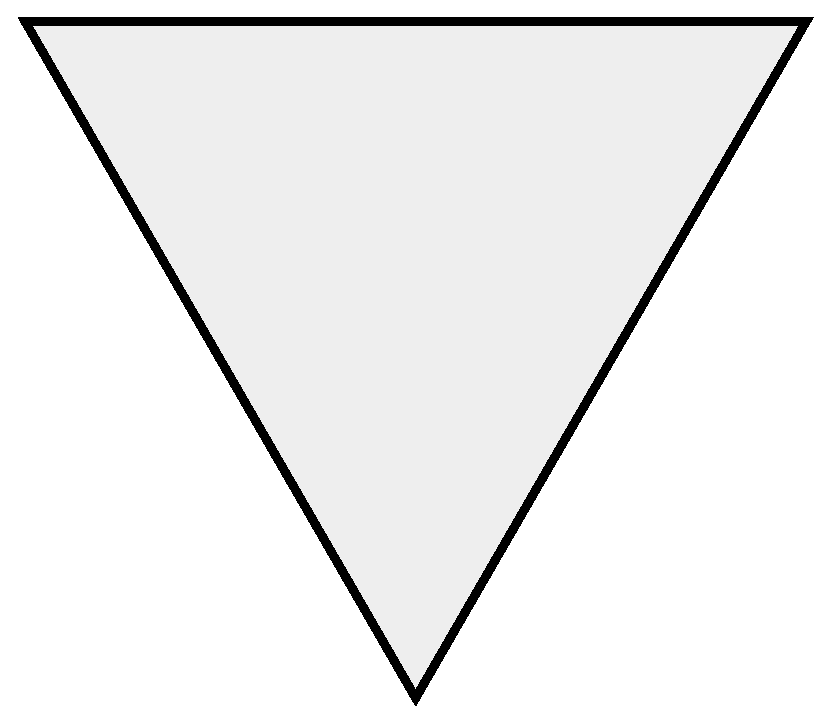
\includegraphics[scale=.15]{pics/Koch_Snowflake-0}
\end{minipage}
\hfill
\begin{minipage}{.24\textwidth}
\centering
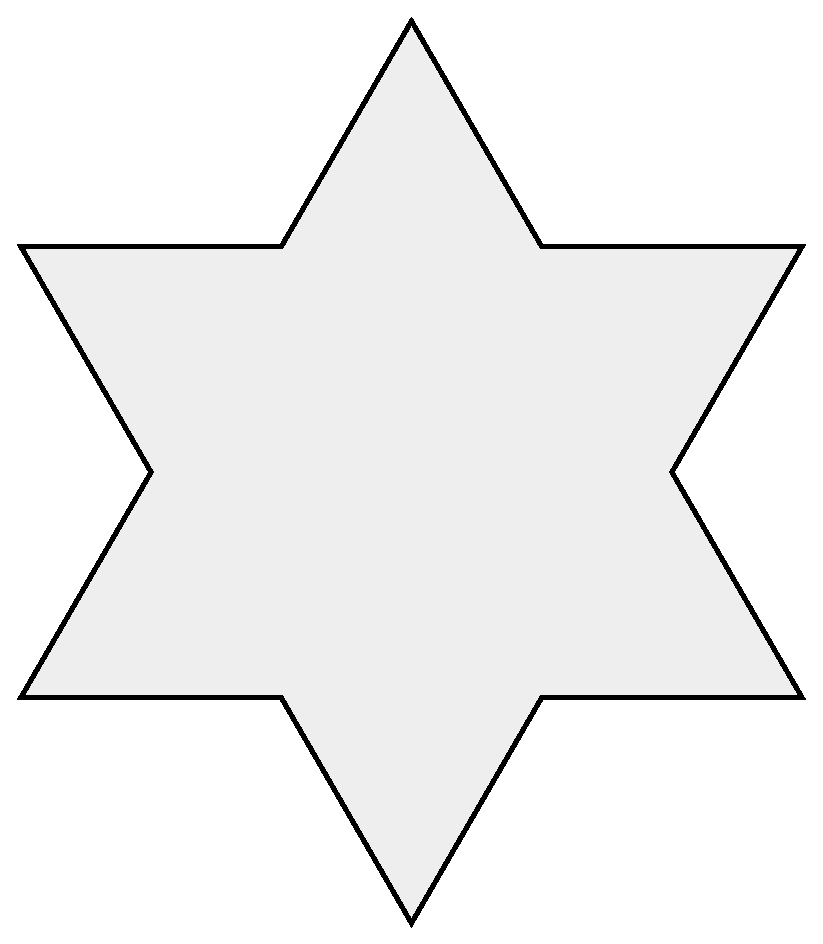
\includegraphics[scale=.15]{pics/Koch_Snowflake-1}
\end{minipage}
\hfill
\begin{minipage}{.24\textwidth}
\centering
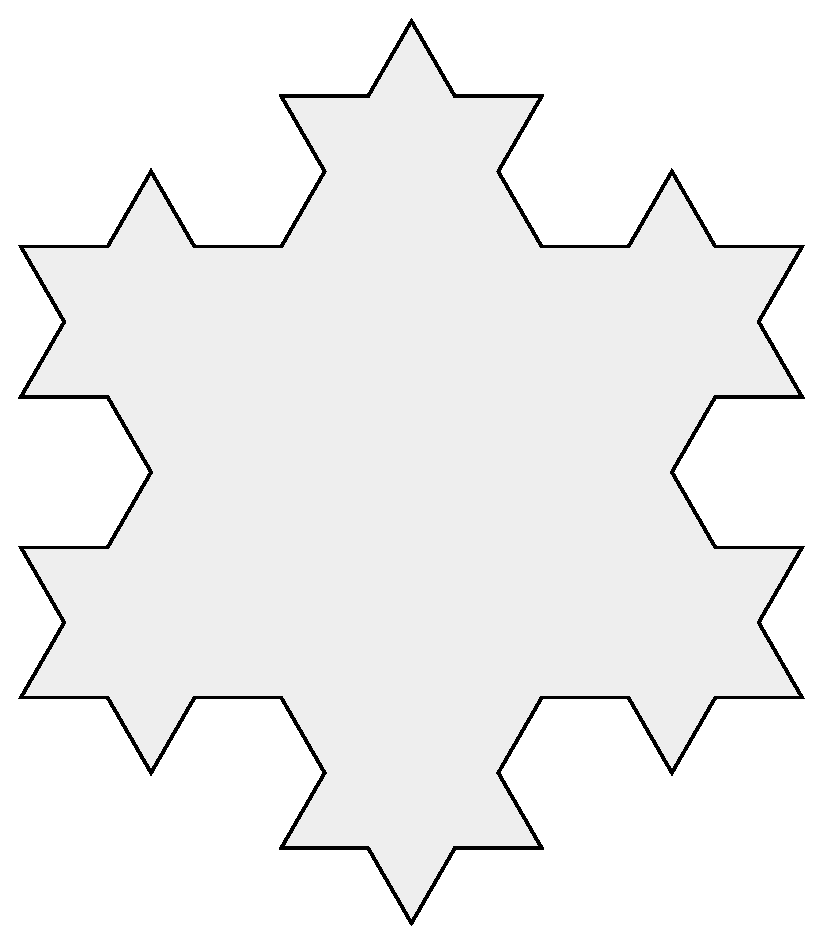
\includegraphics[scale=.15]{pics/Koch_Snowflake-2}
\end{minipage}
\hfill
\begin{minipage}{.24\textwidth}
\centering
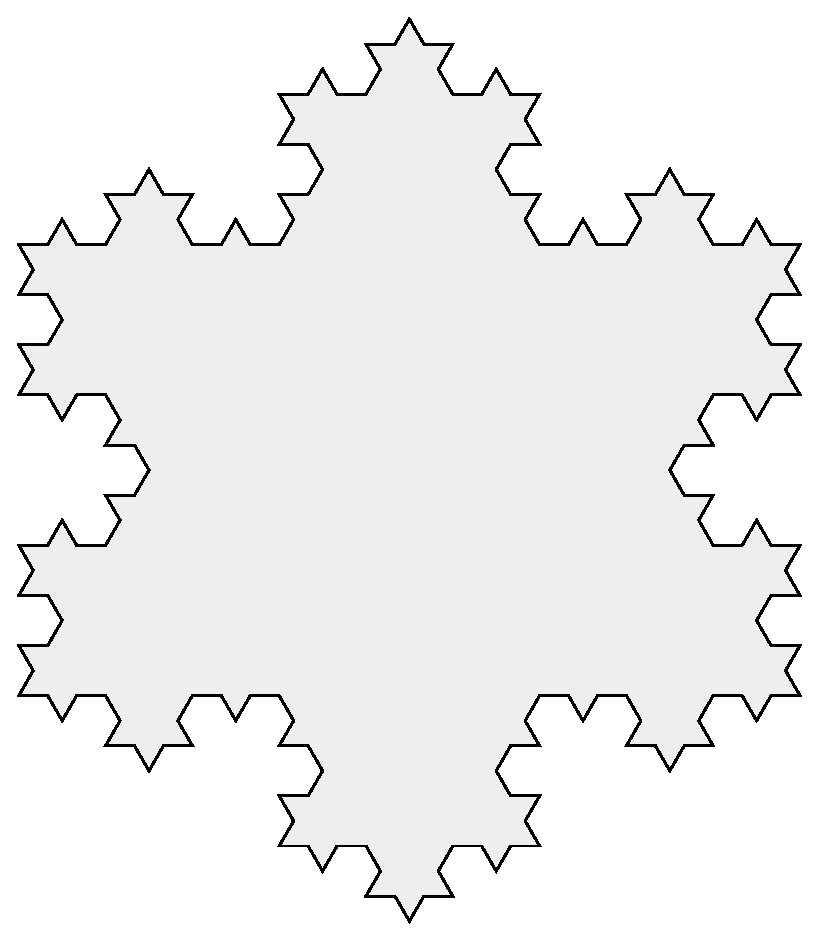
\includegraphics[scale=.15]{pics/Koch_Snowflake-3}
\end{minipage}
\end{figure}
Few first iterations of the construction are shown on the diagram.
The Koch snowflake is the boundary of the union of all the polygons.


\begin{thm}{Exercise}\label{ex:nonrectifiable-curve}
\begin{enumerate}[(a)]
\item Show that Koch snowflake is a closed simple curve; that is, it admits a homeomorphism to a circle.
\item\label{ex:nonrectifiable-curve:b} Show that Koch snowflake is not rectifiable. 
\end{enumerate}
\end{thm}


\section*{Arc length parametrization}

We say that a parametrized curve $\gamma$ has an \emph{arc length parametrization}\footnote{which is also called \emph{natural parametrization}}
if for any two values of parameters $t_1<t_2$, the value $t_2-t_1$ is the length of $\gamma|_{[t_1,t_2]}$; that is, the closed arc of $\gamma$ from $t_1$ to $t_2$.

Note that a smooth space curve $\gamma(t)=(x(t),y(t),z(t))$ has arc length parametrization if and only if it has unit velocity vector at all times;
that is 
\[|\gamma'(t)|=\sqrt{x'(t)^2+y'(t)^2+z'(t)^2}=1;\]
by that reason arc length parametrization of smooth curves with also called \emph{unit-speed curves}.
Note that smooth unit-speed curves are automatically regular.


Any rectifiable curve can be parameterized by arc length.
For a parametrized smooth curve $\gamma$, the arc length parameter $s$ can be written as an integral
\[s(t)=\int_{t_0}^t |\gamma'(\tau)|\cdot d\tau.\]
Note that $s(t)$ is a smooth increasing function.
Further by fundamental theorem of calculus, $s'(t)=|\gamma'(t)|$.
Therefore if $\gamma$ is regular, then $s'(t)\ne0$ for any parameter value $t$.
By inverse function theorem (\ref{thm:inverse}) the inverse function $s^{-1}(t)$ is also smooth.
Therefore $\gamma\circ s^{-1}$ --- the reparametrization  of $\gamma$ by arclength  $s$ --- remains smooth and regular.

Most of the time we use $s$ for an arc length parameter of a curve.

\begin{thm}{Exercise}\label{ex:arc-length-helix}
Reparametrize the helix 
\[\gamma_{a,b}(t)=(a\cdot\cos t,a\cdot \sin t, b\cdot t)\]
by arc length.
\end{thm}

We will be interested in the properties of curves that are invariant under a reparametrization.
Therefore we can always assume that the given smooth regular curve comes with a arc length parametrization.
A good property of arc length parametrizations is that it is almost canonical --- these parametrizations differ only by a sign and additive constant.
On the other hand, often it is impossible to find an arc length parametrization in a closed form which makes it hard to use it calculations;
usually it is more convenient to use the original parametrization.

\section*{Convex curves}

A simple plane curve is called \emph{convex} if it bounds a convex region.

\begin{thm}{Proposition}\label{prop:convex-curve}
Assume a convex closed curve $\alpha$ lies inside the domain bounded by a closed simple plane curve $\beta$.
Then
\[\length\alpha\le \length\beta.\]
\end{thm}

Note that it is sufficient to show that for any polygon  $P$ inscribed in $\alpha$ there is a polygon $Q$ inscribed in $\beta$ with 
$\perim P\le \perim Q$, where $\perim P$ denotes the perimeter of $P$.

Therefore it is sufficient to prove the following lemma.


\begin{thm}{Lemma}\label{lem:perimeter}
Let $P$ and $Q$ be polygons.
Assume $P$ is convex and $Q\supset P$.
Then 
\[\perim P\le \perim Q.\]

\end{thm}


\begin{wrapfigure}{r}{24 mm}
\vskip-4mm
\centering
\includegraphics{mppics/pic-7}
%\caption*{}
\end{wrapfigure}

\parit{Proof.}
Note that by the triangle inequality,
the inequality
\[\perim P\le \perim Q\]
holds
if $P$ can be obtained from $Q$ by cutting it along a chord;
that is, a line segment with ends on the boundary of $Q$ that lies in $Q$.


Note that there is an increasing sequence of polygons 
$$P=P_0\subset P_1\subset\dots\subset P_n=Q$$
such that $P_{i-1}$ obtained from $P_{i}$ by cutting along a chord.
Therefore 
\begin{align*}
\perim P=\perim P_0&\le\perim P_1\le\dots
\\
\dots&\le\perim P_n=\perim Q
\end{align*}
and the lemma follows.
\qeds

\begin{thm}{Corollary}
Any convex closed plane curve is rectifiable.  
\end{thm}

\parit{Proof.}
Any closed curve is bounded; that is, it lies in a sufficiently large square.
Indeed the curve can be described as an image of a loop $\alpha\:[0,1]\to\RR^2$, $\alpha(t)=(x(t),y(t))$.
The coordinate functions $x(t)$ and $y(t)$ are continous functions defined on $[0,1]$.
Therefore the absolute values of both of these functions are bounded by some constant $C$.
That is $\alpha$ lies in the square defined by the inequalities $|x|\le C$ and $|y|\le C$.

By Proposition~\ref{prop:convex-curve}, the length of the curve can not exceed the perimeter of the square $8\cdot C$, whence the result.
\qeds

Recall that convex hull of a set $X$ is the smallest convex set that contains $X$; in other words convex hull is the intersection of all convex sets containing $X$.

\begin{thm}{Exercise}\label{ex:convex-hull}
Let $\alpha$ be a closed simple plane curve.
Denote by $K$ the convex hull of $\alpha$; let $\beta$ be the boundary curve of $K$.
Show that 
\[\length \alpha\ge \length \beta.\]

Try to show that the statement holds for arbitrary closed plane curve $\alpha$, assuming that $X$ has nonempty interior.
\end{thm}


\section*{Crofton formulas*}

Consider a plane curve $\alpha\:[a,b]\to\RR^2$.
Given a unit vector $u$, denote by $\alpha_u$ the curve that follows orthogonal projections of $\alpha$ to the line in the direction $u$;
that is 
\[\alpha_u(t)=\langle u,\alpha(t)\rangle\cdot u.\]

Note that 
\[|\alpha'(t)|=|\langle u,\alpha'(t)\rangle|\] for any $t$.
Note that for any plane vector the magnitude of its average projection is proportional to its magnitude with coefficient; that is,
\[|w|=k\cdot \overline{|w_u|},\]
where $\overline{|w_u|}$ denotes the average value of $|w_u|$ for all unit vectors $u$.
(The value $k$ is the average value of $|\cos\phi|$ for $\phi\in [0,2\cdot\pi]$; it can be found by integration, but soon we will show another way to find it.)

If the curve $\alpha$ is smooth, then according to Exercise~\ref{ex:integral-length}
\begin{align*}
\length\alpha
&=\int_a^b|\alpha'(t)|\cdot dt=
\\
&=\int_a^b  k\cdot \overline{|\alpha_u'(t)|}\cdot dt=
\\
&=k\cdot \overline{\length\alpha_u}.
\end{align*}
This formula and its relatives are called Crofton formulas.
To find the coefficient $k$ one can apply it for the unit circle: the left hand side is $2\cdot\pi$ --- this is the length of unit circle.
Note that for any unit vector $u$, the curve $\alpha_u$ runs back and forth along an interval of length 2.
Therefore $\length\alpha_u=4$ and hence its average value is also 4.
It follows that the coefficient $k$ has to satisfy the equation $2\cdot \pi =k\cdot 4$; whence 
\[
\length\alpha
=\tfrac\pi2\cdot \overline{\length\alpha_u}.
\]

The Crofton's formula holds for arbitrary rectifiable curves, not necessary smooth; it can be proved using Exercises~\ref{adex:integral-length}.

\begin{thm}{Exercise}\label{ex:convex-croftons}
Show that any closed plane curve $\alpha$ has length at least $\pi\cdot s$, where $s$ is the average of pojections of $\alpha$ to lines.
Moreover the equality holds if and only if $\alpha$ is convex.

Use this statement to give another solution of Exercise~\ref{ex:convex-hull}.
\end{thm}

\begin{thm}{Advanced exercise}\label{adex:more-croftons}
Show that the length of space curve is proportional to the average length of its projections to all lines and to planes.
Find the coefficients in each case.
\end{thm}


\begin{thm}{Advanced exercises}\label{adex:integral-length}
\begin{enumerate}[(a)]
\item Show that the formula \ref{eq:length} holds for any Lipschitz curve $\alpha\:[a,b]\z\to\RR^3$.
\item Construct a simple curve $\alpha\:[a,b]\to\RR^3$ such that the velocity vector $\alpha'(t)$ is defined and bounded for almost all $t\in [a,b]$, but the formula \ref{eq:length} does not hold.

\end{enumerate}
\end{thm}

\parit{Hint:} Use theorems of Rademacher and Lusin (\ref{thm:rademacher} and \ref{thm:lusin}).

\section*{Semicontinuity of length}

Recall that the lower limit 
of a sequence of real numbers $(x_n)$ is denoted by
\[\liminf_{n\to\infty} x_n.\] 
It is defined as the lowest partial limit; that is, the lowest possible limit of a subsequence of $(x_n)$.
The lower limit is defined for any sequence of real numbers and it lies in the exteded real line $[-\infty,\infty]$


\begin{thm}{Theorem}\label{thm:length-semicont}
Length is a lower semi-continuous with respect to pointwise convergence of curves. 

More precisely, assume that a sequence
of curves $\alpha_n\:[a,b]\to \spc{X}$ in a metric space $\spc{X}$ converges pointwise 
to a curve $\alpha_\infty\:[a,b]\to \spc{X}$;
that is, $\alpha_n(t)\z\to\alpha_\infty(t)$ for any fixed $t\in[a,b]$ as $n\to\infty$. 
Then 
$$\liminf_{n\to\infty} \length\alpha_n \ge \length\alpha_\infty.\eqlbl{eq:semicont-length}$$
\end{thm}



\begin{wrapfigure}{r}{20 mm}
\vskip-0mm
\centering
\includegraphics{mppics/pic-6}
\end{wrapfigure}


Note that the inequality \ref{eq:semicont-length} might be strict.
For example the diagonal $\alpha_\infty$ of the unit square 
can be  approximated by a sequence of stairs-like
polygonal curves $\alpha_n$
with sides parallel to the sides of the square ($\alpha_6$ is on the picture).
In this case
\[\length\alpha_\infty=\sqrt{2}\quad
\text{and}\quad \length\alpha_n=2\]
for any $n$.

\parit{Proof.}
Fix a partition $a=t_0<t_1<\dots<t_k=b$.
Set 
\begin{align*}\Sigma_n
&\df
|\alpha_n(t_0)-\alpha_n(t_1)|+\dots+|\alpha_n(t_{k-1})-\alpha_n(t_k)|.
\\
\Sigma_\infty
&\df
|\alpha_\infty(t_0)-\alpha_\infty(t_1)|+\dots+|\alpha_\infty(t_{k-1})-\alpha_\infty(t_k)|.
\end{align*}

Note that $\Sigma_n\to \Sigma_\infty$ as $n\to\infty$
and $\Sigma_n\le\length\alpha_n$ for each $n$.
Hence
$$\liminf_{n\to\infty} \length\alpha_n \ge \Sigma_\infty.\eqlbl{>=Sigma-infty}$$

If $\alpha_\infty$ is rectifiable, we can assume that 
\begin{align*}
\length\alpha_\infty<\Sigma_\infty+\eps.
\end{align*}
for any given $\eps>0$.
By \ref{>=Sigma-infty} it follows that 
$$\liminf_{n\to\infty} \length\alpha_n > \length\alpha_\infty-\eps$$
for any $\eps>0$; whence \ref{eq:semicont-length} follows.

It remains to consider the case when $\alpha_\infty$ is not rectifiable; 
that is $\length\alpha_\infty=\infty$.
In this case we can choose a partition so that $\Sigma_\infty>L$ for any real number $L$.
By \ref{>=Sigma-infty} it follows that 
$$\liminf_{n\to\infty} \length\alpha_n > L$$
for any $L$; whence 
\[\liminf_{n\to\infty}\length\alpha_n=\infty\]
and \ref{eq:semicont-length} follows.
\qeds

\section*{Length metric}

Let $\spc{X}$ be a metric space.
Given two points $x,y$ in $\spc{X}$, denote by $d(x,y)$ the exact lower bound for lengths of all paths connecting $x$ to $y$; if there is no such path we assume that $d(x,y)=\infty$.

Note that function $d$ satisfies all the axioms of metric except it might take infinite value.
Therefore if any two points in $\spc{X}$ can be connected by a rectifiable curve, then $d$ defines a new metric on $\spc{X}$; in this case $d$ is called \emph{induced length metric}.

Evidently $d(x,y)\ge |x-y|$ for any pair of points $x,y\in \spc{X}$.
If the equality holds for any pair, then then the metric is called \emph{length metric} and the space is called \emph{length-metric space}.

Most of the time we consider length-metric spaces.
In particular the Euclidean space is a length-metric space.
A subspaces $A$ of length-metric space $\spc{X}$ might be not a lenght-metric space;
the induced length distance between points $x$ and $y$ in the subspace $A$ will be denoted as $|x-y|_A$;
that is $|x-y|_A$ is the exact lower bound for the length of paths in $A$.

\begin{thm}{Exercise}\label{ex:intrinsic-convex}
Let $A\subset \RR^3$ be a closed subset.
Show that $A$ is convex if and only if
\[|x-y|_A=|x-y|_{\RR^3}.\]
\end{thm}

\begin{thm}{Exercise}\label{ex:S1-intrinsic}
Let us denote by $\SS^1$ the unit circle in the plane; that is,
\[\SS^1=\set{(x,y)\in\RR^3}{x^2+y^2=1}.\]
Show that
\[|u-v|_{\SS^1}=\measuredangle(u,v)\df\arccos\langle u,v\rangle\]
for any $u,v\in \SS^1$.
\end{thm}

\section*{Spherical curves}

A space curve $\gamma$ is called \emph{spherical} if it runs in the unit sphere;
that is, $|\gamma(t)|=1$ for any $t$.

\begin{thm}{Exercise}\label{ex:S2-intrinsic}
Let us denote by $\SS^2$ the unit sphere in the space; that is,
\[\SS^2=\set{(x,y,z)\in\RR^3}{x^2+y^2+z^2=1}.\]
Show that
\[|u-v|_{\SS^2}=\measuredangle(u,v)\df\arccos\langle u,v\rangle\]
for any $u,v\in \SS^2$.
\end{thm} %???spherical geometry

\parit{Hint:} Use Exercise~\ref{ex:S1-intrinsic} and the following map $f\:(r,\theta,\phi)\mapsto (r,\theta,0)$ in spherical coordinates. Note that $f$ is distance nonexpanding and it maps $\RR^3$ to a half-plane and $\SS^2$ to one of its meridians.

\begin{thm}{Hemisphere lemma}\label{lem:hemisphere}
Any closed curve of length $<2\cdot \pi$ in $\SS^2$ lies in an open hemisphere. 
\end{thm}

This lemma is a keystone in the proof of Fenchel's theorem given below.
The lemma is not as simple as you might think --- try to prove it yourself.
I learned the following proof from Stephanie Alexander.

\parit{Proof.}
Let $\alpha$ be a closed curve in $\mathbb{S}^2$ of length $2\cdot\ell$.

%???+PIC

Assume $\ell<\pi$.

\begin{wrapfigure}{r}{35 mm}
\vskip-0mm
\centering
\includegraphics{mppics/pic-52}
\caption*{The north hemisphere corresponds to the disc and the south hemisphere to the complement of the disc.}
\end{wrapfigure}

Let us divide $\alpha$ into two arcs $\alpha_1$ and $\alpha_2$ of length $\ell$, with endpoints $p$ and $q$. 
According to Exercise~\ref{ex:S2-intrinsic}, $\measuredangle(p,q)\le\ell<\pi$.
Denote by $z$ be the midpoint between $p$ and $q$ in $\mathbb{S}^2$;
that is $z$ is the midpoint of an equator arc from $p$ to $q$. 
We claim that $\alpha$ lies in the open north hemisphere with north pole at $z$.  
If not, $\alpha$ intersects the equator in a point, say $r$.
Without loss of generality we may assume that $r$ lies on~$\alpha_1$. 

Rotate the arc $\alpha_1$ by angle $\pi$ around the line thru $z$ and the center of the sphere.
The obtained arc $\alpha_1^{*}$ together with $\alpha_1$ forms a closed curve of length $2\cdot \ell$ that passes thru $r$ and its antipodal point $r^{*}$.
Therefore
\[\tfrac12\cdot\length \alpha=\ell\ge \measuredangle(r,r^{*})=\pi,\] 
a contradiction.
\qeds

\begin{thm}{Exercise}\label{ex:antipodal}
Describe a simple closed spherical curve that does not pass thru a pair of antipodal points and does not lie in any hemisphere.
\end{thm}


\begin{thm}{Exercise}\label{ex:bisection-of-S2}
Suppose that a closed simple spherical curve $\alpha$ divides $\SS^2$ into two regions of equal area.
Show that 
\[\length\alpha\ge2\cdot\pi.\]
\end{thm}


\begin{thm}{Exercise}\label{ex:flaw}
Consider the following problem, find a flaw in the given solution.
Come up with a correct argument.
\end{thm}

 
\parbf{Problem.}
Suppose that a closed plane curve $\alpha$ has length at most 4.
Show that $\alpha$ lies in a unit disc.

\parit{Wrong solution.}
Note that it is sufficient to show that diameter of $\alpha$ is at most 2;
that is, the distance between any two pairs of points $p$ and $q$ of $\alpha$ an not exceed $2$.

The length of $\alpha$ can not be smaller then the closed inscribed polygonal line which goes from $p$ to $q$ and back to $p$.
Therefore 
\[2\cdot |p-q|\le\length \alpha\le 4.\]
\qedsf

\begin{thm}{Advanced exercises} \label{adex:crofton}
Given points $v,w\in\SS^2$, denote by $w_v$ the closest point to $w_u$ on the equator with pole at $v$;
in other words, it $w^\perp$ is the projection of $w$ to the plane perpendicular to $v$, then $w_v$ is the unit vector in the direction of $w^\perp$.
The vector $w_v$ is defined if $w\ne\pm v$.

\begin{enumerate}
\item \label{adex:crofton:crofton}
Show that for any spherical curve $\alpha$ we have that
\[\length\alpha=\overline{\length\alpha_v},\]
where $\overline{\length\alpha_v}$ denotes the average length for all $v\in \SS^2$.
(This is a spherical analog of Crofton's formula.)
\item\label{adex:crofton:hemisphere} Give another proof of hemisphere lemme using part (\ref{adex:crofton:crofton}). 
\end{enumerate}
 
\end{thm}


\chapter{Curvature}

\section*{Acceleration of a unit-speed curve}

Recall that any regular smooth curve can be parameterized by its arc-length.
The obtained parameterized curve, say $\gamma$, remains to be smooth and it has unit speed; 
that is, $|\gamma'(s)|=1$ for all $s$.
The following proposition states that in this case
the acceleration vector stays perpendicular to the velocity vector.

\begin{thm}{Proposition}\label{prop:a'-pertp-a''}
Assume $\gamma$ is a smooth unit-speed space curve.
Then $\gamma'(s)\perp \gamma''(s)$ for any $s$.
\end{thm}

The scalar product (also known as dot product) of two vectors $\vec v$ and $\vec w$ will be denoted by $\langle \vec v,\vec w\rangle$.
Recall that the derivative of a scalar product satisfies the product rule;
that is, if $\vec v=\vec v(t)$ and $\vec w=\vec w(t)$ are smooth vector-valued functions of a real parameter $t$, then
\[\langle \vec v,\vec w\rangle'=\langle \vec v',\vec w\rangle+\langle \vec v,\vec w'\rangle.\]

\parit{Proof.}
The identity $|\gamma'|=1$ can be rewritten as $\langle\gamma',\gamma'\rangle=1$.
Differentiating both sides, 
\[2\cdot\langle\gamma'',\gamma'\rangle=\langle\gamma',\gamma'\rangle'=0,\]
whence $\gamma''\perp\gamma'$.
\qeds

\section*{Curvature}

For a unit-speed smooth space curve $\gamma$ the magnitude of its acceleration $|\gamma''(s)|$ is called its \emph{curvature} at the time $s$.
\label{page:curvature}
If $\gamma$ is simple, then we can say that $|\gamma''(s)|$ is the curvature at the point $p=\gamma(s)$ without ambiguity.
The curvature is usually denoted by $\kur(s)$ or $\kur(s)_\gamma$ and in the case of simple curves it might be also denoted by $\kur(p)$ or $\kur(p)_\gamma$.

The curvature measures how fast the curve turns;
if you drive along a plane curve, then curvature describes the position of your steering wheel at the given point (note that it does not depend on your speed).

In general, the term \emph{curvature} is used for anything that measures how much a \emph{geometric object} deviates from being \emph{straight};
for curves, it measures how fast it deviates from a straight line.

\begin{thm}{Exercise}\label{ex:curvature-of-spherical-curve}
Show that any regular smooth unit-speed spherical curve has curvature at least 1 at each time.
\end{thm}

\section*{Tangent indicatrix}

Let $\gamma$ be a regular smooth space curve.
Let us consider another curve 
\[\tan(t)=\tfrac{\gamma'(t)}{|\gamma'(t)|}\eqlbl{eq:tantrix}\] 
called \emph{tangent indicatrix} of $\gamma$.
Note that $|\tan(t)|=1$ for any $t$;
that is, $\tan$ is a spherical curve.


If $s\mapsto \gamma(s)$ is a unit-speed parametrization, then $\tan(s)=\gamma'(s)$.
In this case we have the following expression for curvature: 
\[\kur(s)\z=|\tan'(s)|\z=|\gamma''(s)|.\]

When $\gamma$ is not necessarily parameterized by arc-length, then
\[ \kur(t)=\frac{|\tan'(t)|}{|\gamma'(t)|}.\eqlbl{eq:curvature}\]
Indeed, for an arc-length parametrization $s(t)$ we have $s'(t)=|\gamma'(t)|$.
Therefore
\begin{align*}
\kur(t)&=\left|\frac{d\tan}{ ds}\right|=
\\
&=|\tfrac{d\tan}{ dt}|/|\tfrac{ds}{ dt}|=
\\
&=\frac{|\tan'(t)|}{|\gamma'(t)|}.
\end{align*}
It follows that the indicatrix of a smooth regular curve $\gamma$ is regular if the curvature of $\gamma$ does not vanish.

\begin{thm}{Exercise}\label{ex:curvature-formulas}
Use the formulas \ref{eq:tantrix} and \ref{eq:curvature} to show that 
for any smooth regular space curve $\gamma$ we have the following expressions for its curvature:

\begin{subthm}{ex:curvature-formulas:a} \[\kur(t)=\frac{|\vec w(t)|}{|\gamma'(t)|^2},\]
where $\vec w(t)$ denotes the projection of $\gamma''(t)$ to the plane normal to $\gamma'(t)$;
\end{subthm}

\begin{subthm}{ex:curvature-formulas:b}
\[\kur(t)=\frac{|\gamma''(t)\times \gamma'(t)|}{|\gamma'(t)|^{3}},\]
where $\times$ denotes the \emph{vector product} (also known as \emph{cross product}).
\end{subthm}

\end{thm}


\begin{thm}{Exercise}\label{ex:curvature-graph}
Apply the formulas in the previous exercise to show that if $f$ is a smooth real function,
then its graph $y=f(x)$  has curvature
\[\kur(p)=\frac{|f''(x)|}{(1+f'(x)^2)^{\frac32}}\]
at the point $p=(x,f(x))$.
\end{thm}

\section*{Tangent curves}

Let $\gamma$ be a smooth regular space curve and $\tan$ its tangent indicatrix.
The line thru $\gamma(t)$ in the direction of $\tan(t)$ is called the \emph{tangent line} at~$t$.

The tangent line could be also defined as a unique line that has that has \emph{first order of contact} with $\gamma$ at $s$;

that is, $\rho(\ell)=o(\ell)$, where $\rho(\ell)$ denotes the distance from $\gamma(s+\ell)$ to the line.

We say that smooth regular curve $\gamma_1$ at $s_1$ is \emph{tangent} to a smooth regular curve $\gamma_2$ at $s_2$
if $\gamma_1(s_1)=\gamma_2(s_2)$ and the tangent line of $\gamma_1$ at $s_1$ coincides with the tangent line of $\gamma_2$ at $s_2$;
if both curves are simple we can also say that they are tangent at the point $p=\gamma_1(s_1)\z=\gamma_2(s_2)$ without ambiguity.


\section*{Total curvature}

Let $\gamma\:\mathbb{I}\to\RR^3$ be a smooth unit-speed curve and $\tan$ its tangent indicatrix.
The integral 
\[\tc\gamma:=\int_{\mathbb{I}}\kur(s)\cdot ds\]
is called \emph{total curvature of}\label{page:total curvature of:smooth-def}
$\gamma$.

When $\gamma$ is not parameterized by arc-length, by a change of variables, the above integral takes the form

\[\tc\gamma:=\int_{\mathbb{I}}\kur( \gamma (t) ) | \gamma ' (t) | \cdot ds   \eqlbl{eq:tocurv} \]


\begin{thm}{Exercise}\label{ex:helix-curvature}
Find the curvature of the helix \[\gamma_{a,b}(t)=(a\cdot \cos t,a\cdot \sin t,b\cdot t),\] its tangent indicatrix and the total curvature of its  arc for $t\in[0,2\cdot\pi]$.
\end{thm}

\begin{thm}{Observation}\label{obs:tantrix}
The total curvature of a smooth regular curve is the length of its tangent indicatrix.
\end{thm}

\parit{Proof.}
Combine \ref{eq:tocurv} and \ref{eq:curvature}.
\qedsf %???other cases --- colsed curves, semiopen intervals...


\begin{thm}{Fenchel's theorem}\label{thm:fenchel}
The total curvature of any closed regular space curve is at least $2\cdot\pi$.
\end{thm}

\parit{Proof.}
Fix a closed regular space curve $\gamma$;
we can assume that it is described by a unit-speed loop $\gamma\:[a,b]\to \RR^3$;
in this case $\gamma(a)=\gamma(b)$ and $\gamma'(a)=\gamma'(b)$.

Consider its tangent indicatrix $\tan=\gamma'$.
Recall that $|\tan(s)|=1$ for any $s$; that is, $\tan$ is a closed spherical curve.

Let us show that $\tan$ cannot lie in a hemisphere.
Assume the contrary; without loss of generality we can assume that $\tan$ lies in the north hemisphere defined by the inequality $z>0$ in $(x,y,z)$-coordinates.
It means that $z'(t)>0$ for all $t$, where $\gamma(t)=(x(t), y(t), z(t))$.
Therefore 
\[z(b)-z(a)=\int_a^bz'(s)\cdot ds>0.\]
In particular, $\gamma(a)\ne \gamma(b)$, a contradiction.

Applying the observation (\ref{obs:tantrix}) and the hemisphere lemma (\ref{lem:hemisphere}), we get  
\[\tc\gamma=\length \tan\ge2\cdot\pi.\]
\qedsf

\begin{thm}{Exercise}\label{ex:length>=2pi}
Show that a closed space curve $\gamma$ with curvature at most~$1$ cannot be shorter than the unit circle;
that is, 
\[\length\gamma\ge 2\cdot \pi.\]

\end{thm}


\begin{thm}{Advanced exercise}\label{ex:gamma/|gamma|}
Suppose that $\gamma$ is a smooth regular space curve that does not pass thru the origin.
Consider the spherical curve defined as $\sigma(t)=\frac{\gamma(t)}{|\gamma(t)|}$ for any $t$.
Show that 
\[\length \sigma< \tc\gamma+\pi.\]
Moreover, if $\gamma$ is closed, then
\[\length \sigma\le \tc\gamma.\]
\end{thm}

Note that the last inequality gives an alternative proof of Fenchel's theorem.
Indeed, without loss of generality we can assume that the origin lies on a chord of $\gamma$.
In this case the closed spherical curve $\sigma$ goes from a point to its antipode and comes back; 
it takes length $\pi$ each way, 
whence 
\[\length\sigma\ge 2\cdot\pi.\]



\section*{Piecewise smooth curves}



Assume $\alpha\:[a,b]\to \RR^3$ and $\beta\:[b,c]\z\to \RR^3$ are two curves such that $\alpha(b)=\beta(b)$.
Then one can combine these two curves into one $\gamma\:[a,c]\z\to \RR^3$ by the rule 
\[\gamma(t)=
\begin{cases}
\alpha(t)&\text{if}\quad t\le b,
\\
\beta(t)&\text{if}\quad t\ge b.
\end{cases}
\]
The obtained curve $\gamma$ is called the 
\emph{concatenation} of $\alpha$ and $\beta$. %briefly $\gamma=\alpha{*}\beta$.
(The condition $\alpha(b)=\beta(b)$ ensures that the map $t\mapsto\gamma(t)$ is continuous.)

The same definition of concatenation can be applied if $\alpha$ and/or $\beta$ are defied on semiopen intervals 
$(a,b]$ and/or $[b,c)$.

\begin{wrapfigure}{o}{25 mm}
\vskip-2mm
\centering
\includegraphics{mppics/pic-54}
\end{wrapfigure}

The concatenation can be also defined if the end point of the first curve coincides with the starting point of the second curve;
if this is the case, then the time intervals of both curves can be shifted so that they fit together. 

If in addition $\beta(c)=\alpha(a)$, then we can do cyclic concatination of these curves;
this way we obtain a closed curve.

If $\alpha'(b)$ and $\beta'(b)$ are defined, then the angle $\theta=\measuredangle(\alpha'(b),\beta'(b))$ is called \emph{external angle} of $\gamma$ at time $b$.
If $\theta=\pi$, then we say that $\gamma$ has a \emph{cusp} at  time $b$.

Clearly, the assumption that the intervals $[a,b]$ and $[b,c]$ fit together is not essential, and we can concatenate any two curves $\alpha$ and $\beta$ as long as the endpoint of $\alpha$ coincides with the starting point of~$\beta$. 

A space curve $\gamma$ is called \emph{piecewise smooth and regular} if it can be presented as an iterated concatination of a finite number of smooth regular curves; if $\gamma$ is closed, then the  concatination is assumed to be cyclic.

If $\gamma$ is a concatination of smooth regular arcs $\gamma_1,\dots,\gamma_n$, then the total curvature of $\gamma$ is defined as a sum of the total curvatures of $\gamma_i$ and the external angles;
that is, 
\[\tc\gamma=\tc{\gamma_1}+\dots+\tc{\gamma_n}+\theta_1+\dots+\theta_{n-1}\]
where $\theta_i$ is the external angle at the joint between $\gamma_i$ and $\gamma_{i+1}$;
if $\gamma$ is closed, then 
\[\tc\gamma=\tc{\gamma_1}+\dots+\tc{\gamma_n}+\theta_1+\dots+\theta_{n},\]
where $\theta_n$ is the external angle at the joint between $\gamma_n$ and $\gamma_1$.

In particular, for a smooth regular loop $\gamma:[a,b] \to \mathbb{R}^3$, the total curvature of the corresponding closed curve $\hat\gamma$ is defined as
\[\tc{\hat\gamma}\df\tc\gamma + \theta,\]
where $\theta=\measuredangle(\gamma'(a),\gamma'(b))$.

\begin{thm}{Generalized Fenchel's theorem}\label{thm:gen-fenchel}
Let $\gamma$ be a closed piecewise smooth regular space curve.
Then 
\[\tc\gamma\ge2\cdot\pi.\]

\end{thm}

\parit{Proof.}
Suppose $\gamma$ is a cyclic concatenation of $n$ smooth regular arcs $\gamma_1,\dots,\gamma_n$.
Denote by $\theta_1,\dots,\theta_n$ its external angles.
We need to show that
\[\tc{\gamma_1}+\dots+\tc{\gamma_n}+\theta_1+\dots+\theta_n\ge2\cdot\pi.\eqlbl{eq:gen-fenchel}\]

Consider the tangent indicatrix $\tan_1,\dots,\tan_n$ for each arc $\gamma_1,\dots,\gamma_n$;
these are smooth spherical arcs.

The same argument as in the proof of Fenchel's theorem, shows that the curves $\tan_1,\dots,\tan_n$ cannot lie in an open hemisphere.

Note that the spherical distance from the end point of $\tan_i$ to the starting point of $\tan_{i+1}$ is equal to the external angle $\theta_i$ (we enumerate the arcs modulo $n$, so $\gamma_{n+1}=\gamma_1$).
Let us connect the end point of $\tan_i$ to the starting point of $\tan_{i+1}$ by a short arc of a great circle in the sphere.
This way we get a closed spherical curve that is $\theta_1+\dots+\theta_n$ longer then the total length of $\tan_1,\dots,\tan_n$.

Applying the hemisphee lemma (\ref{lem:hemisphere}) to the obtained closed curve, we get that
\[\length\tan_1+\dots+\length\tan_n+\theta_1+\dots+\theta_n\ge 2\cdot\pi.\]
Applying the observation (\ref{obs:tantrix}), we get \ref{eq:gen-fenchel}.
\qedsf

\begin{thm}{Chord lemma}\label{lem:chord}
Let $\ell$ be the chord to a smooth regular arc $\gamma\:[a,b]\to\RR^3$.
Assume $\gamma$ meets $\ell$ at angles $\alpha$ and $\beta$ at $\gamma (a)$ and $\gamma (b)$, respectively;
that is 
\[\alpha=\measuredangle(\vec w,\gamma'(a))\quad\text{and}\quad \beta=\measuredangle(\vec w,\gamma'(b)),\]
where $\vec w=\gamma(b)-\gamma(a)$.
Then 
\[\tc\gamma\ge \alpha+\beta.\eqlbl{tc>a+b}\] 

\end{thm}

\begin{wrapfigure}{o}{45 mm}
\vskip-0mm
\centering
\includegraphics{mppics/pic-53}
\vskip0mm
\end{wrapfigure}

%??? is it really due to Reshetnyak???

\parit{Proof.}
Let us parameterize the chord $\ell$ from $\gamma(b)$ to $\gamma(a)$ and consider the cyclic concatenation $\bar\gamma$ of $\gamma$ and $\ell$.
The closed curve $\bar\gamma$ has two external angles $\pi-\alpha$ and $\pi-\beta$.
Since the curvature of $\ell$ vanishes, we get 
\[\tc{\bar\gamma}=\tc\gamma+(\pi-\alpha)+(\pi-\beta).\]
According to the generalized Fenechel's theorem (\ref{thm:gen-fenchel}),
$\tc{\bar\gamma}\ge 2\cdot\pi$;
hence \ref{tc>a+b} follows.
\qeds

\begin{thm}{Exercise}\label{ex:chord-lemma-optimal}
Show that the estimate in the chord lemma is optimal.
That is, given two points $p, q$ and two unit vectors $u,v$ in $\RR^3$,
show that there is a smooth regular curve $\gamma$ that starts at $p$ in the direction $\vec u$ and ends at $q$ in the direction $\vec v$ such that 
$\tc\gamma$ is arbitrarily close to $\measuredangle(\vec w,\vec u)+\measuredangle(\vec w,\vec v)$, where $\vec w=q-p$.

\end{thm}

\section*{Polygonal lines} 

Polygonal lines are a particular case of piecewise smooth regular curves;
each arc in its concatenation is a line segment.
Since the curvature of a line segment vanishes, the total curvature of a polygonal line is the sum of its external angles.

\begin{thm}{Exercise}\label{ex:monotonic-tc}
Let $a,b,c,d$ and $x$ be distinct points in $\RR^3$.
Show that the total curvature of the polygonal line $abcd$ cannot exceed the total curvature of $abxcd$; that is, 
\[\tc {abcd} \leq \tc {abxcd}.\]

Use this statement to show that any closed polygonal line has curvature at least $2\cdot\pi$.
\end{thm}



\begin{thm}{Proposition}\label{prop:inscribed-total-curvature}
Assume a polygonal line $\beta=p_0\dots p_n$ is inscribed in a smooth regular curve $\gamma$.
Then 
\[\tc\gamma\ge \tc{\beta}.\]
Moreover if $\gamma$ is closed we allow the inscribed polygonal line $\beta$ to be closed.

\end{thm}

\parit{Proof.}
Since the curvature of line segments vanishes, 
the total curvature of polygonal line is the sum of external angles $\theta_i=\pi-\measuredangle p_{i-1}p_ip_{i+1}$.

\begin{wrapfigure}{o}{40 mm}
\vskip-0mm
\centering
\includegraphics{mppics/pic-55}
\vskip0mm
\end{wrapfigure}

Assume $p_i=\gamma(t_i)$.
Set 
\begin{align*}
\vec w_i&=p_{i+1}-p_i,& \vec v_i&=\gamma'(t_i),
\\
\alpha_i&=\measuredangle (\vec w_i,\vec v_i),&\beta_i&=\measuredangle (\vec w_{i-1},\vec v_i).
\end{align*}
In the case of a closed curve we use indexes modulo $n$, in particular $p_{n+1}\z=p_1$.

Note that $\theta_i=\measuredangle (\vec w_{i-1},\vec w_i)$.
By triangle inequality for angles \ref{thm:spherical-triangle-inq}, we get that
\[\theta_i\le \alpha_i+\beta_i.\]
By the chord lemma, the total curvature of the arc of $\gamma$ from $p_i$ to $p_{i+1}$ is at least $\alpha_i+\beta_{i+1}$. 

Therefore if $\gamma$ is a closed curve, we have
\begin{align*}
\tc{\beta}&=\theta_1+\dots+\theta_n\le 
\\
&\le\beta_1+\alpha_1+\dots+\beta_n+\alpha_n = 
\\
&=(\alpha_1+\beta_2)+\dots+(\alpha_n+\beta_1) \le 
\\
&\le \tc\gamma.
\end{align*}
If $\gamma$ is an arc, the argument is analogous:
\begin{align*}
\tc{\beta}&=\theta_1+\dots+\theta_{n-1}\le 
\\
&\le\beta_1+\alpha_1+\dots+\beta_{n-1}+\alpha_{n-1} \le
\\
&\le (\alpha_0+\beta_1)+\dots+(\alpha_{n-1}+\beta_n) \le 
\\
&\le \tc\gamma.
\end{align*}
\qedsf

\begin{thm}{Exercise}\label{ex:sef-intersection}

\begin{subthm}{ex:sef-intersection:<2pi}Draw a smooth regular plane curve $\gamma$ which has a self-intersection, such that $\tc\gamma<2\cdot\pi$.
\end{subthm}

\begin{subthm}{ex:sef-intersection:>pi} Show that if a smooth regular curve $\gamma\:[a,b]\to\RR^3$ has a self-intersection, then $\tc\gamma>\pi$.
\end{subthm}

\end{thm}

\begin{thm}{Proposition}\label{prop:fenchel=}
The equality case in the Fenchel's theorem holds only for convex plane curves;
that is, if the total curvature of a smooth regular space curve $\gamma$ equals $2\cdot\pi$, then $\gamma$ is a convex plane curve.
\end{thm}

The proof is an application of Proposition~\ref{prop:inscribed-total-curvature}.

\parit{Proof.}
Consider an inscribed quadraliteral $abcd$ in $\gamma$.
By the definition of total curvature, we have that
\begin{align*}
\tc{abcd}&=(\pi-\measuredangle dab)+(\pi-\measuredangle abc)+(\pi-\measuredangle bcd)+(\pi-\measuredangle cda)=
\\
&=4\cdot\pi -(\measuredangle dab+\measuredangle abc+\measuredangle bcd+\measuredangle cda))
\end{align*}


Note that 
\[
\measuredangle abc\le\measuredangle abd+ \measuredangle dbc
\quad\text{and}\quad
\measuredangle cda\le\measuredangle cdb+ \measuredangle bda.
\eqlbl{eq:spheric-triangle}
\]

The sum of angles in any triangle is $\pi$, so combining these inequalities, we get that 
\begin{align*}
\tc{abcd}&\ge 4\cdot \pi 
- (\measuredangle dab+\measuredangle abd+ \measuredangle bda)
-(\measuredangle bcd+\measuredangle cdb +\measuredangle dbc)=
\\
&=2\cdot\pi.
\end{align*}

\begin{wrapfigure}{r}{40 mm}
\vskip-7mm
\centering
\includegraphics{mppics/pic-56}
\vskip0mm
\end{wrapfigure}

By \ref{prop:inscribed-total-curvature},
\[\tc{abcd}\le \tc\gamma\le 2\cdot\pi.\]
Therefore we have equalities in \ref{eq:spheric-triangle}.
It means that the point $d$ lies in the angle $abc$ 
and the point $b$ lies in the angle $cda$.
That is, $abcd$ is a convex plane quadrilateral.

It follows that any quadrilateral inscribed in $\gamma$ is a convex plane quadrilateral.
Therefore all points of $\gamma$ lie in a fixed plane and the domain bounded by $\gamma$ in that plane is convex;
that is, $\gamma$ is a convex plane curve. %???more
\qeds

\begin{wrapfigure}{o}{30 mm}
\vskip-4mm
\centering
\includegraphics{mppics/pic-20}
\vskip0mm
\end{wrapfigure}

\begin{thm}{Exercise}\label{ex:quadrisecant}
Suppose that a closed curve $\gamma$ crosses a line at four points $a$, $b$, $c$ and $d$.
Assume that these points appear on the line in the order $a$, $b$, $c$, $d$
and they appear on the curve $\gamma$ in the order $a$, $c$, $b$, $d$.
Show that 
\[\tc\gamma\ge 4\cdot\pi.\]

\end{thm}

Lines crossing a curve at four points as in the above exercise are called \emph{alternating quadrisecants}.
It turns out that any \emph{nontrivial knot} admits an alternating quadrisecant \cite{denne};
according to the exercise the latter implies the so-called \emph{F\'ary--Milnor theorem} --- the total curvature any knot exceeds $4\cdot \pi$.

\section*{Bow lemma}

\begin{thm}{Lemma}\label{lem:bow}
Let $\gamma_1\:[a,b]\to\RR^2$ and $\gamma_2\:[a,b] \to\RR^3$ be two smooth unit-speed curves.
Suppose that $\kur(s)_{\gamma_1}\ge\kur(s)_{\gamma_2}$ for any $s$ 
and the curve
$\gamma_1$ is a simple arc of a convex curve; that is, it runs in the boundary of a covex plane figure.
Then the distance between the ends of $\gamma_1$ cannot exceed the  distance between the ends of $\gamma_2$; that is,
\[|\gamma_1(b)-\gamma_1(a)|\le |\gamma_2(b)-\gamma_2(a)|.\]

\end{thm}

The following exercise states that the condition that $\gamma_1$ is a convex arc is necessary.
It is instructive to do this exercise before reading the proof of the lemma.

\begin{thm}{Exercise}\label{ex:anti-bow}
Construct a simple smooth unit-speed plane curves $\gamma_1,\gamma_2\:[a,b]\to\RR^2$ such that 
that $\kur(s)_{\gamma_1}>\kur(s)_{\gamma_2}$ for any $s$ and
\[|\gamma_1(b)-\gamma_1(a)|> |\gamma_2(b)-\gamma_2(a)|.\]
\end{thm}


\begin{wrapfigure}{o}{36 mm}
\vskip-7mm
\centering
\includegraphics{mppics/pic-57}
\vskip0mm
\end{wrapfigure}

\parit{Proof.}
Denote by $\tan_1$ and $\tan_2$ the tangent indicatrixes of $\gamma_1$ and $\gamma_2$, respectively.

Let $\gamma_1(s_0)$ be the point on $\gamma_1$ furthest to the line 
thru $\gamma(a)$ and $\gamma(b)$.
Consider two unit vectors 
\[\vec u_1=\tan_1(s_0)=\gamma_1'(s_0)
\quad\text{and}\quad
\vec u_2=\tan_2(s_0)=\gamma_2'(s_0).\]
By construction, the vector $\vec u_1$ is parallel to $\gamma(b)-\gamma(a)$, in particular
\[|\gamma_1(b)-\gamma_1(a)|=\langle \vec u_1,\gamma_1(b)-\gamma_1(a)\rangle \]

Since $\gamma_1$ is an arc of a convex curve, its indicatrix $\tan_1$ runs in one direction along the unit circle.
Suppose $s\le s_0$, then 
\begin{align*}
\measuredangle(\gamma'_1(s),\vec u_1)&=\measuredangle(\tan_1(s),\tan_1(s_0))=
\\
&=\length (\tan_1|_{[s,s_0]})=
\\
&=\int_s^{s_0}|\tan_1'(t)|\cdot d t=
\\
&=\int_s^{s_0}\kur_1(t)\cdot d t\ge
\\
&\ge
\int_s^{s_0}\kur_2(t)\cdot d t=
\\
&=\int_s^{s_0}|\tan_2'(t)|\cdot d t= 
\\
&=\length (\tan_1|_{[s,s_0]})\ge
\\
&\ge \measuredangle(\tan_2(s),\tan_2(s_0))=
\\
&= \measuredangle(\gamma'_2(s),\vec u_2).
\end{align*}
That is, 
\[\measuredangle(\gamma'_1(s),\vec u_1)\ge \measuredangle(\gamma'_2(s),\vec u_2)\]
if $s\ge s_0$.
The same argument shows that 
\[\measuredangle(\gamma'_1(s),\vec u_1)\ge \measuredangle(\gamma'_2(s),\vec u_2)\eqlbl{<gamma',u>}\]
for $s\ge s_0$; therefore the inequality holds for any $s$.

Since $\vec u_1$ is a unit vector parallel to $\gamma_1(b)-\gamma_1(a)$, we have that
\[|\gamma_1(b)-\gamma_1(a)|=\langle \vec u_1,\gamma_1(b)-\gamma_1(a)\rangle\]
and since $\vec u_2$ is a unit vector, we have that
\[|\gamma_2(b)-\gamma_2(a)|\ge\langle \vec u_2,\gamma_2(b)-\gamma_2(a)\rangle\]

Integrating \ref{<gamma',u>}, we get 
\begin{align*}
|\gamma_1(b)-\gamma_1(a)|&=\langle \vec u_1,\gamma_1(b)-\gamma_1(a)\rangle=
\\
&=\int_a^b\langle \vec u_1,\gamma'_1(s)\rangle\cdot ds \le 
\\
&\le\int_a^b\langle \vec u_2,\gamma'_2(s)\rangle\cdot ds =
\\
&=\langle \vec u_2,\gamma_2(b)-\gamma_2(a)\rangle \le
\\
&\le |\gamma_2(b)-\gamma_2(a)|.
\end{align*}
Hence the result.\qeds

\begin{thm}{Exercise}\label{ex:length-dist}
Let $\gamma\:[a,b]\to \RR^3$ be a smooth regular curve and $0<\theta\le\tfrac\pi2$.
Assume 
\[\tc\gamma\le 2\cdot\theta.\]

\begin{subthm}{ex:length-dist:>} Show that
\[|\gamma(b)-\gamma(a)|> \cos\theta\cdot\length\gamma.\]
\end{subthm}

\begin{subthm}{} Use part \ref{SHORT.ex:length-dist:>} to give another solution of \ref{ex:sef-intersection:>pi}.
\end{subthm}

\begin{subthm}{} Show that the inequality in \ref{SHORT.ex:length-dist:>} is optimal; that is, given 
$\theta$ there is a smooth regular curve $\gamma$ such that $\frac{|\gamma(b)-\gamma(a)|}{\length\gamma}$ is arbitrarily close to $\cos\theta$.
\end{subthm}

\end{thm}



\begin{thm}{Exercise}\label{ex:schwartz}
Let $p$ and $q$ be points in a unit circle dividing it in two arcs with lengths $\ell_1<\ell_2$.
Suppose the space curve $\gamma$ connects $p$ to $q$ and has curvature at most 1. Show that either
\[\length \gamma\le \ell_1
\quad\text{or}\quad
\length \gamma\ge \ell_2.
\]
\end{thm} %H. A. Schwartz???

The following exercise generalizes \ref{ex:length>=2pi}.

\begin{thm}{Exercise}\label{ex:loop}
Suppose $\gamma\:[a,b]\to \RR^3$ is a smooth regular loop with curvature at most 1.
Show that 
\[\length\gamma\ge2\cdot\pi.\]

\end{thm}


\section*{DNA inequality*}

Recall that the curvature of a spherical curve is at least $1$
(Exercise~\ref{ex:curvature-of-spherical-curve}).
In particular, the length of a spherical curve cannot exceed its total curvature.
The following theorem shows that the same inequality holds for \emph{closed} curves in a unit ball.

\begin{thm}{Theorem}\label{thm:DNA}
Let $\gamma$ be a smooth regular closed curve that lies in a unit ball.
Then 
\[\tc\gamma\ge \length\gamma.\]

\end{thm}

This theorem was proved by Don Chakerian \cite{chakerian};
for plane curves it was proved earlier by Istv\'{a}n F\'{a}ry \cite{fary-DNA}.
We present the proof given by Don Chakerian in \cite{chakerian-short};
few other proofs of this theorem are discussed by Serge Tabachnikov~\cite{tabachnikov}.

\parit{Proof.}
Without loss of generality we can assume the curve is described by a loop $\gamma\:[0,\ell]\to\RR^3$ parameterized by its arc-length, so $\ell=\length\gamma$.
We can also assume that the origin is the center of the ball.
It follows that
\[\langle\gamma'(s),\gamma'(s)\rangle=1,\qquad |\gamma(s)|\le 1\]
and in particular 
\[\begin{aligned}
\langle\gamma''(s),\gamma(s)\rangle&\ge -|\gamma''(s)|\cdot|\gamma(s)|\ge
\\
&\ge-\kur(s)
\end{aligned}\eqlbl{eq:<gamma'',gamma>>=-k}\]
for all $s$. Since $\gamma$ is a smooth closed curve, we have 
$\gamma'(0)=\gamma'(\ell)$ and $\gamma(0)=\gamma(\ell)$.
Applying \ref{eq:<gamma'',gamma>>=-k}, we get that
\begin{align*}
0&=\langle\gamma(\ell),\gamma'(\ell)\rangle
-
\langle\gamma(0),\gamma'(0)\rangle=
\\
&=\int_0^\ell\langle\gamma(s),\gamma'(s)\rangle'\cdot ds=
\\
&=\int_0^\ell\langle\gamma'(s),\gamma'(s)\rangle\cdot ds+\int_0^\ell\langle\gamma(s),\gamma''(s)\rangle\cdot ds\ge
\\
&\ge \ell-\tc\gamma,
\end{align*}
whence the result.
\qeds

\section*{Nonsmooth curves*}

\begin{thm}{Theorem}\label{thm:total-curvature=}
For any regular smooth space curve $\gamma$ we have that 
\[\tc\gamma=\sup\{\tc\beta\},\]
where the supremum is taken over all polygonal lines~$\beta$ inscribed in $\gamma$
(if $\gamma$ is closed we assume that so is $\beta$).
\end{thm}

This theorem is a refinement of Proposition~\ref{prop:inscribed-total-curvature}.
It shows that the following definition of total curvature of arbitrary curves, 
generalize the original definition that works only for (piecewise) smooth and regular curves.

We say that a parameterized curve is trivial if it is constant; that is, it stays at one point.

\begin{thm}{Definition}\label{def:total-curv-poly}
The total curvature of a nontrivial parameterized space curve $\gamma$ is the exact upper bound on the total curvatures of inscribed nondegenerate polygonal lines;
if $\gamma$ is closed, then we assume that the inscribed polygonal lines are closed as well.
\end{thm}

\parit{Proof of the theorem.}
Note that the inequality 
\[\tc\gamma\ge \tc\beta\]
follows from \ref{prop:inscribed-total-curvature};
it remains to show 
\[\tc\gamma\le\sup\{\tc\beta\}. \eqlbl{eq:tc=<tc}\]

Let $\gamma\:[a,b]\to\RR^3$ be a smooth curve.
Fix a partition $a\z=t_0\z<\dots<t_k=b$ and consider the corresponding inscribed polygonal line $\beta=p_0\dots p_k$.
(If $\gamma$ is closed, then  $p_0=p_k$ and $\beta$ is closed as well.)

Let $\tau=\xi_1\dots\xi_k$ be a spherical polygonal line
with the vertexes $\xi_i\z=\tfrac{p_i-p_{i-1}}{|p_i-p_{i-1}|}$.
We can assume that $\tau$ has constant speed on each arc and $\tau(t_i)=\xi_i$ for each $i$. 
The spherical polygonal line $\tau$ will be called tangent indicatrix for $\beta$.

Consider a sequence of finer and finer partitions, denote by $\beta_n$ and $\tau_n$ the corresponding inscribed polygonal lines and their tangent indicatrixes.
Note that since $\gamma$ is smooth, the idicatrixes $\tau_n$ converge pointwise to $\tan$ --- the tangent indicatrix of $\gamma$.
By the semi-continuity of the length (\ref{thm:length-semicont}), we get that  
\begin{align*}
\tc\gamma&=\length \tan\le  
\\
&\le \liminf_{n\to\infty}\length \tau_n=
\\
&= \liminf_{n\to\infty}\tc {\beta_n}\le
\\
&\le \sup\{\tc\beta\}.
\end{align*}
\qeds

\begin{thm}{Exercise}\label{ex:tc-semicontinuous}
Show that the total curvature is lower semi-continuous with respect to pointwise convergence of curves.
That is, if a sequence
of curves $\gamma_n\:[a,b]\to \RR^3$ converges pointwise 
to a nontrivial curve $\gamma_\infty\:[a,b]\z\to \RR^3$, then 
\[\liminf_{n\to\infty} \tc{\gamma_n} \ge \tc{\gamma_\infty}.\]
\end{thm}

\begin{thm}{Exercise}\label{ex:gen-fenchel}
Generalize Fenchel's theorem to all nontrivial closed space curves.
That is, show that \[\tc\gamma\ge2\cdot\pi\]
for any  closed space curve $\gamma$ (not necessary piecewise smooth and regular).
\end{thm}

\begin{thm}{Exercise}\label{ex:tc-length}

\begin{subthm}{ex:tc-length:rectifiable}
Assume that a curve $\gamma\:[a,b]\to\RR^3$ has finite total curvature.
Show that $\gamma$ is rectifiable.
\end{subthm}

\begin{subthm}{ex:tc-length:example}
Construct a rectifiable curve $\gamma\:[a,b]\to\RR^3$ that has infinite total curvature.
\end{subthm}

\end{thm}

For more on curves of finite total curvature read \cite{aleksandrov-reshetnyak,sullivan-curves}. 

\section*{DNA inequality revisited*}

In this section we will give an alternative proof of the DNA inequality (\ref{thm:DNA}) that works for arbitrary, not necessarily smooth, curves.
In the proof we use \ref{def:total-curv-poly} to define the total curvature;
according to \ref{thm:total-curvature=}, it is more general than the smooth definition given on page \pageref{page:total curvature of:smooth-def}.

\parit{Alternative proof of \ref{thm:DNA}.}
We will show that 
\[\tc\gamma> \length\gamma.\]
for any closed polygonal line $\gamma=p_1\dots p_{n}$ in a unit ball.
It implies the theorem since in any nontrivial closed curve we can inscribe a closed polygonal line with arbitrary close total curvature and length.

The indexes are taken modulo $n$, in particular $p_{n}=p_0$, $p_{n+1}=p_1$ and so on.
Denote by $\theta_i$ the external angle of $\gamma$ at $p_i$;
that is,
\[\theta_i=\pi-\measuredangle p_{i-1}p_ip_{i+1}.\]

Denote by $o$ the center of the ball.
Consider a sequence of $n+1$ plane triangles
\begin{align*}
\triangle q_0s_0q_1
&\cong 
\triangle p_0op_1,
\\
\triangle q_1s_1q_2
&\cong 
\triangle p_1op_2,
\\
&\dots
\\
\triangle q_{n}s_nq_{n+1}
&\cong 
\triangle p_nop_{n+1},
\end{align*}
such that the points $q_0,q_1,\dots,q_{n+1}$ lie on one line in that order and all the points $s_0,\dots,s_n$ lie on one side from this line.

\begin{figure}[h!]
\vskip-0mm
\centering
\includegraphics{mppics/pic-16}
\vskip0mm
\end{figure}

Since $p_0=p_n$ and $p_1=p_{n+1}$, we have that
\[\triangle q_{n}s_nq_{n+1}\cong 
\triangle p_nop_{n+1}=\triangle p_0op_1\cong\triangle q_{0}s_0q_1,\]
so $s_0q_0q_ns_n$ is a parallelogram.
Therefore
\begin{align*}
|s_0-s_1|+\dots+|s_{n-1}-s_n|
&\ge|s_n-s_0|=
\\
&=|q_0-q_n|=
\\
&=|p_0-p_1|+\dots+|p_{n-1}-p_n|
\\
&=\length \gamma.
\end{align*}

Since $|q_i-s_{i-1}|=|q_i-s_i|=|p_i-o|\le 1$, we have that
\[\measuredangle s_{i-1}q_is_i>|s_{i-1}-s_i|\]%???angle
for each $i$.
Therefore
\begin{align*}
\theta_i&=\pi-\measuredangle p_{i-1}p_ip_{i+1}\ge
\\
&\ge\pi-\measuredangle p_{i-1}p_io-\measuredangle op_ip_{i+1}=
\\
&=\pi-\measuredangle q_{i-1}q_is_{i-1}-\measuredangle s_iq_iq_{i+1}=
\\
&=\measuredangle s_{i-1}q_is_i>
\\
&>|s_{i-1}-s_i|.
\end{align*}
That is, 
\[\theta_i>|s_{i-1}-s_i|\]
for each $i$.

It follows that
\begin{align*}
\tc \gamma
&=\theta_1+\dots+\theta_n>
\\
&> |s_{0}-s_1|+\dots |s_{n-1}-s_n|\ge 
\\
&\ge\length \gamma.
\end{align*}
Hence the result.
\qeds


Let us mention the following closely related statement:

\begin{thm}{Theorem}
Suppose a closed regular smooth curve $\gamma$ lies in a convex figure of perimeter $2\cdot \pi$.
Then 
\[\tc\gamma\ge \length\gamma.\]

\end{thm}

This statement was conjectured by Serge Tabachnikov~\cite{tabachnikov}.
Despite the simplicity of the formulation, the proof is annoyingly difficult;
it was proved by Jeffrey Lagarias and Thomas Richardson \cite{lagarias-richardso}; later a simpler proof was given by Alexander Nazarov and Fedor Petrov~\cite{nazarov-petrov}.


\chapter{Torsion}
\label{chap:torsion}

This chapter provides mostly a practice in computations.
Except for the definitions in Section \ref{sec:frenet-frame},
it will not be used in the sequel.
\section{Frenet frame}\label{sec:frenet-frame}

Let $\gamma$ be a smooth regular space curve.
Without loss of generality, we may assume that $\gamma$ has an arc-length parametrization,
so the velocity vector $\tan(s)=\gamma'(s)$ is unit.

Assume its curvature does not vanish at some time $s$;
in other words, $\gamma''(s)\ne 0$.
Then we can define the so-called \index{normal vector}\emph{normal vector} at $s$ as
\[\norm(s)=\frac{\gamma''(s)}{|\gamma''(s)|}.\]
Note that 
\[\tan'(s)=\gamma''(s)=\kur(s)\cdot\norm(s).\]\index{10tnb@$\tan$, $\norm$, $\bi$}

According to \ref{prop:a'-pertp-a''}, $\norm(s)\perp \tan(s)$.
Therefore the vector product 
\[\bi(s)=\tan(s)\times \norm(s)\]
is a unit vector;
moreover the triple $\tan(s),\norm(s),\bi(s)$ an oriented orthonormal basis in $\RR^3$;
in particular, we have that
\[\begin{aligned}
\langle\tan,\tan\rangle&=1,
&
\langle\norm,\norm\rangle&=1,
&
\langle\bi,\bi\rangle&=1,
\\
\langle\tan,\norm\rangle&=0,
&
\langle\norm,\bi\rangle&=0,
&
\langle\bi,\tan\rangle&=0.
\end{aligned}
\eqlbl{eq:orthornomal}
\]

The orthonormal basis $\tan(s),\norm(s),\bi(s)$ is called the \index{Frenet frame}\emph{Frenet frame} at $s$; the vectors in the frame are called \index{tangent}\emph{tangent}, \index{normal}\emph{normal} and \index{binormal}\emph{binormal} respectively.
Note that the frame $\tan(s),\norm(s),\bi(s)$ is defined only if $\kur(s)\ne 0$.

The plane $\Pi_s$ thru $\gamma(s)$ spanned by vectors $\tan(s)$ and $\norm(s)$ is called the \index{osculating!plane}\emph{osculating plane} at $s$;
equivalently it can be defined as a plane thru $\gamma(s)$ that is perpendicular to the binormal vector $\bi(s)$.
This is the unique plane that has a \index{order of contact}\emph{second order of contact} with $\gamma$ at $s$;
that is, $\rho(\ell)=o(\ell^2)$, where $\rho(\ell)$ denotes the distance from $\gamma(s+\ell)$ to $\Pi_s$.

\section{Torsion}

Let $\gamma$ be a smooth unit-speed space curve
and $\tan(s),\norm(s),\bi(s)$ be its Frenet frame.
The value 
\[\tor(s)=\langle \norm'(s),\bi(s)\rangle\]\index{10tau@$\tor$}
is called the \index{torsion}\emph{torsion} of $\gamma$ at $s$.

Note that the torsion $\tor(s_0)$ is defined if $\kur(s_0)\z\ne0$.
Indeed, since the function $s\mapsto \kur(s)$ is continuous, 
$\kur(s_0)\z\ne 0$ implies that $\kur(s)\z\ne 0$ for all $s$ near $s_0$.
Therefore the Frenet frame is also defined in an open interval containing $s_0$.
Clearly $\tan(s)$, $\norm(s)$ and $\bi(s)$ depend smoothly on $s$ in their domains of definition.
Therefore $\norm'(s_0)$ is defined and so is the torsion $\tor(s_0)=\langle \norm'(s_0),\bi(s_0)\rangle$.


\begin{thm}{Exercise}\label{ex:helix-torsion}
Given real numbers $a$ and $b$, calculate the curvature and the torsion of the helix
\[\gamma_{a,b}(t)=(a\cdot \cos t,a\cdot\sin t, b\cdot t).\]

Conclude that for any $\kur>0$ and $\tor$ there is a helix with constant curvature $\kur$ and torsion $\tor$.
\end{thm}


\section{Frenet formulas}

Assume that the Frenet frame $\tan(s),\norm(s),\bi(s)$ of a curve $\gamma$ is defined at $s$.
Recall that 
\[\tan'=\kur\cdot \norm.
\eqlbl{eq:frenet-tau}\]
Let us find the remaining derivatives $\norm'$ and $\bi'$ in the frame $\tan,\norm,\bi$.

First let us show that
\[\norm'=-\kur\cdot\tan+\tor\cdot\bi.\eqlbl{eq:frenet-nu}\]

Since the frame $\tan,\norm,\bi$ is orthonormal, the above formula is equivalent to the following three identities:
\[\begin{aligned}
\langle \norm',\tan\rangle&=-\kur,
&
\langle \norm',\norm\rangle&=0,
&
\langle \norm',\bi\rangle&=\tor,
\end{aligned}\eqlbl{eq:<N',?>}\]
The last identity follows from the definition of torsion.
The second one is a consequence of the identity $\langle \norm,\norm\rangle\z=1$ in \ref{eq:orthornomal}. 
By differentiating the identity $\langle\tan,\norm\rangle\z=0$ in \ref{eq:orthornomal}
we get 
\[\langle\tan',\norm\rangle+\langle\tan,\norm'\rangle=0.\]
Applying \ref{eq:frenet-tau}, we get the first equation in \ref{eq:<N',?>}.

Differentiating the third identity in \ref{eq:orthornomal}, we get that $\bi'\perp\bi$.
Taking further derivatives of the other identities with $\bi$ in \ref{eq:orthornomal}, we get that 
\begin{align*}
\langle\bi',\tan\rangle&=-\langle\bi,\tan'\rangle=-\kur\cdot\langle\bi,\norm\rangle=0,
\\
\langle\bi',\norm\rangle&=-\langle\bi,\norm'\rangle=\tor.
\end{align*}
Since the frame $\tan,\norm,\bi$ is orthonormal, it follows that
\[\bi'=-\tor\cdot\norm.\eqlbl{eq:frenet-beta}\]

The equations \ref{eq:frenet-tau}, \ref{eq:frenet-nu} and \ref{eq:frenet-beta} are called \index{Frenet formulas}\emph{Frenet formulas}.
All three can be written as one matrix identity:
\[
\begin{pmatrix}
\tan'
\\
\norm'
\\
\bi'
\end{pmatrix}
=
\begin{pmatrix}
0&\kur&0
\\
-\kur&0&\tor
\\
0&-\tor&0
\end{pmatrix}
\cdot
\begin{pmatrix}
\tan
\\
\norm
\\
\bi
\end{pmatrix}.
\]


Since $\bi$ is the normal vector to the osculating plane, Equation \ref{eq:frenet-beta} shows that the torsion measures how fast the osculating plane rotates when one travels along $\gamma$.




\begin{thm}{Exercise}\label{ex:beta-from-tau+nu}
Deduce the formula \ref{eq:frenet-beta} from  \ref{eq:frenet-tau} and \ref{eq:frenet-nu} by differentiating the identity
$\bi=\tan\times \norm$.
\end{thm}

\begin{thm}{Exercise}\label{ex:torsion=0}
Let $\gamma$ be a regular space curve with nonvanishing curvature.
Show that $\gamma$ lies in a plane if and only if its torsion vanishes.
\end{thm}


\begin{thm}{Exercise} \label{ex:frenet}
Let $\gamma$ be a smooth regular space curve, $\kur$ and $\tor$ its curvature and torsion,
and $\tan,\norm,\bi$ its Frenet frame.
Show that 
\[\bi=\frac{\gamma'\times\gamma''}{|\gamma'\times\gamma''|}
\quad\text{and}\quad
\tor=\frac{\langle\gamma'\times\gamma'',\gamma'''\rangle}{|\gamma'\times\gamma''|^2}.
\]

\end{thm}

\section{Curves of constant slope}

We say that a smooth regular space curve $\gamma$ has \index{constant slope}\emph{constant slope} if its velocity vector makes a constant angle with a fixed direction.
The following theorem was proved by Michel Ange Lancret~\cite{lancret} more than two centuries ago.

\begin{thm}{Theorem}\label{thm:const-slope}
Let $\gamma$ be a smooth regular curve;
denote by $\kur$ and $\tor$ its curvature and torsion.
Suppose $\kur(s)>0$ for all $s$.
Then $\gamma$ has constant slope if and only if the ratio $\tfrac\tor\kur$ is constant.
\end{thm}

The following exercise will guide you thru the proof of the theorem. 

\begin{thm}{Exercise} \label{ex:lancret}
Let $\gamma$ be a smooth regular space curve with nonvanishing curvature, $\tan,\norm,\bi$ 
its Frenet frame and $\kur$, $\tor$ its curvature and torsion.


\begin{subthm}{ex:lancret:a}
Assume that  $\langle \vec w,\tan\rangle$ is constant for a fixed nonzero vector $\vec w$.
Show that 
\[\langle \vec w, \norm\rangle =0.\]
Use it to show that 
\[\langle \vec w, -\kur\cdot\tan+\tor\cdot \bi\rangle =0.\]
Use these two identities to show that $\tfrac\tor\kur$ is constant;
this proves the ``only if'' part of the theorem.
\end{subthm}

\begin{subthm}{ex:lancret:b} Assume $\tfrac\tor\kur$ is constant, show that the vector $\vec w=\tfrac\tor\kur\cdot \tan+\bi$ is constant.
Conclude that $\gamma$ has constant slope; this proves the ``if'' part of the theorem.
\end{subthm}

\end{thm}

Let $\gamma$ be a smooth unit-speed curve and $s_0$ a fixed real number. 
Then the curve 
\[\alpha(s)=\gamma(s)+(s_0-s)\cdot \gamma'(s)\]
is called the \index{evolvent}\emph{evolvent} of $\gamma$.
Note that if $\ell(s)$ denotes the tangent line to $\gamma$ at $s$,
then $\alpha(s)\in \ell(s)$ and $\alpha'(s)\perp \ell$ for all $s$.

\begin{thm}{Exercise}\label{ex:evolvent-constant-slope}
Show that the evolvent of a constant slope curve is a plane curve.
\end{thm}

\section{Spherical curves}

\begin{thm}{Theorem}
Suppose that $\gamma$ is a smooth regular space curve with nonvanishing torsion $\tor$ and (therefore) curvature $\kur$.
Then $\gamma$ lies in a unit sphere if and only if 
the following identity holds true:
\[\left|\frac{\kur'}{\tor}\right|=\kur\cdot\sqrt{\kur^2-1}.\]
\end{thm}

The proof is another application of the Frenet formulas;
we present it in the form of a guided exercise:

\begin{thm}{Exercise}\label{ex:spherical-frenet}
Suppose $\gamma$ is a smooth unit-speed space curve.
Denote by $\tan,\norm,\bi$ its Frenet frame and by $\kur$, $\tor$ its curvature and torsion.

\smallskip

Assume that $\gamma$ is spherical; that is, $|\gamma(s)|=1$ for any $s$.
Show that

\begin{subthm}{ex:spherical-frenet:tau} $\langle\tan,\gamma\rangle=0$; conclude that $\langle\norm,\gamma\rangle^2+\langle\bi,\gamma\rangle^2=1$.
\end{subthm}

\begin{subthm}{ex:spherical-frenet:nu} $\langle\norm,\gamma\rangle=-\tfrac1\kur$;
\end{subthm}

\begin{subthm}{ex:spherical-frenet:beta} $\langle\bi,\gamma\rangle'=\tfrac\tor\kur$.
\end{subthm}

\begin{subthm}{ex:spherical-frenet:beta+}
Use \ref{SHORT.ex:spherical-frenet:beta} to show that if $\gamma$ is closed, then $\tor(s)=0$ for some~$s$.
\end{subthm}

\begin{subthm}{ex:spherical-frenet:kur-tor} Assume that the torsion of $\gamma$ does not vanish.
Use \ref{SHORT.ex:spherical-frenet:tau}--\ref{SHORT.ex:spherical-frenet:beta} to show that 
\[\left|\frac{\kur'}{\tor}\right|=\kur\cdot\sqrt{\kur^2-1}.\]
(It proves the ``only if'' part of the theorem.)
\end{subthm}
Now assume that $\gamma$ is a space curve that satisfies the identity in \ref{SHORT.ex:spherical-frenet:kur-tor}.
\begin{subthm}{ex:spherical-frenet:f} Show that $p=\gamma+\tfrac1\kur\cdot \norm+\tfrac{\kur'}{\kur^2\cdot\tor}\cdot\bi$ is constant; conclude that $\gamma$ lies in the unit sphere centered at $p$.
(It proves the ``if'' part of the theorem.)
\end{subthm}

\end{thm}

For a unit-speed curve $\gamma$ with nonzero curvature and torsion at $s$,
the sphere $\Sigma_s$ with center
\[p(s)=\gamma(s)+\tfrac1{\kur(s)}\cdot \norm(s)+\tfrac{\kur'(s)}{\kur^2(s)\cdot\tor(s)}\cdot\bi(s)\]
and passing thru $\gamma(s)$ is called the \index{osculating sphere}\emph{osculating!sphere} of $\gamma$ at $s$.
This is the unique sphere that has \index{order of contact}\emph{third order of contact} with $\gamma$ at $s$;
that is, $\rho(\ell)=o(\ell^3)$, where $\rho(\ell)$ denotes the distance from $\gamma(s+\ell)$ to $\Sigma_s$.
 
\section{Fundamental theorem of space curves}

\begin{thm}{Theorem}\label{thm:fund-curves}
Let $\kur(s)$ and $\tor(s)$ be two smooth real valued functions defined on a real interval $\mathbb{I}$.
Suppose $\kur(s)>0$ for all $s$.
Then there is a smooth unit-speed curve $\gamma\:\mathbb{I}\to\RR^3$ with curvature $\kur(s)$ and torsion $\tor(s)$ for every $s$.
Moreover $\gamma$ is uniquely defined up to a rigid motion of the space.
\end{thm}

The proof is an application of the theorem on existence and uniqueness of solutions of ordinary differential equations (\ref{thm:ODE}).

\parit{Proof.}
Fix a parameter value $s_0$, a point $\gamma(s_0)$ and an oriented orthonormal frame $\tan(s_0)$, $\norm(s_0)$, $\bi(s_0)$.

Consider the following system of differential equations
\[
\begin{cases}
\gamma'=\tan,
\\
\tan'=\kur\cdot\norm,
\\
\norm'=-\kur\cdot\tan+\tor\cdot\bi,
\\
\bi'=-\tor\cdot\norm.
\end{cases}
\eqlbl{eq:gamma'tan'norm'bi'}
\]
with the initial condition $\gamma(s_0)$ and an oriented orthonormal frame $\tan(s_0)$, $\norm(s_0)$, $\bi(s_0)$.
(The system of equations has four vector equations, so it can be rewritten as a system of 12 scalar equations.)

By \ref{thm:ODE}, this system has a unique solution which is defined in a maximal subinterval $\mathbb{J}\subset \mathbb{I}$ containing $s_0$.
Let us show that actually $\mathbb{J}=\mathbb{I}$.

Observe that 
\[\langle\tan,\tan\rangle'
=
\langle\norm,\norm\rangle'
=
\langle\bi,\bi\rangle'
=
\langle\tan,\norm\rangle'
=
\langle\tan,\bi\rangle'
=
\langle\bi,\tan\rangle'=0.
\]
Indeed,
\begin{align*}
\langle\tan,\tan\rangle'
&=
2\cdot\langle\tan,\tan'\rangle
=
2\cdot\kur\cdot \langle\tan,\norm\rangle
=
0,
\\
\langle\norm,\norm\rangle'
&=
2\cdot\langle\norm,\norm'\rangle
=
-
2\cdot\kur\cdot\langle\norm,\tan\rangle
+
2\cdot\tor\cdot\langle\norm,\bi\rangle
=
0,
\\
\langle\bi,\bi\rangle'
&=
2\cdot\langle\bi,\bi'\rangle
=
-2\cdot\tor\langle\bi,\norm\rangle
=
0,
\\
\langle\tan,\norm\rangle'
&=
\langle\tan',\norm\rangle
+
\langle\tan,\norm'\rangle
=
\kur\cdot\langle\norm,\norm\rangle
-
\kur\cdot\langle\tan,\tan\rangle
+
\tor\cdot\langle\tan,\bi\rangle
=
0,
\\
\langle\norm,\bi\rangle'
&=
\langle\norm',\bi\rangle+\langle\norm,\bi'\rangle
=0,
\\
\langle\bi,\tan\rangle'
&=
\langle\bi',\tan\rangle+\langle\bi,\tan'\rangle
=
-\tor\cdot \langle\norm,\tan\rangle
+\kur\cdot\langle\bi,\norm\rangle
=0.
\end{align*}

It follows that the values 
$\langle\tan,\tan\rangle$,
$\langle\norm,\norm\rangle$,
$\langle\bi,\bi\rangle$,
$\langle\tan,\norm\rangle$,
$\langle\tan,\norm\rangle$,
$\langle\bi,\tan\rangle$
are constant functions of $s$.
Since we choose $\tan(s_0)$, $\norm(s_0)$, $\bi(s_0)$ to be an oriented orthonormal frame, we have that the triple $\tan(s)$, $\norm(s)$, $\bi(s)$ is an oriented orthonormal frame for any $s$. In particular, $|\gamma'(s)|=1$ for all $s$.

Assume $\mathbb{J} \varsubsetneq \mathbb{I}$. Then an end of $\mathbb{J}$, say $a$, lies in the interior of $\mathbb{I}$.
By Theorem~\ref{thm:ODE}, at least one of the values $\gamma(s)$, $\tan(s)$, $\norm(s)$, $\bi(s)$
escapes to infinity as $s\to a$.
But this is impossible since the vectors $\tan(s)$, $\norm(s)$, $\bi(s)$ remain unit and $|\gamma'(s)|=|\tan(s)|=1$ --- a contradiction.
Hence $\mathbb{J}= \mathbb{I}$.

Now assume there are two curves $\gamma_1$ and $\gamma_2$ with the given curvature and torsion functions.
Applying a motion of the space we can assume that $\gamma_1(s_0)=\gamma_2(s_0)$ and the Frenet frames of the curves coincide at $s_0$.
Then $\gamma_1=\gamma_2$ by the uniqueness of  solutions to the system (\ref{thm:ODE}).
Hence the last statement follows.
\qeds

\begin{thm}{Exercise}\label{ex:cur+tor=helix}
Assume a curve $\gamma\:\RR\to\RR^3$ has constant curvature and torsion.
Show that $\gamma$ is a helix, possibly degenerate to a circle;
that is, in a suitable coordinate system we have
\[\gamma(t)=(a\cdot \cos t,a\cdot\sin t, b\cdot t)\]
for some constants $a$ and $b$.
\end{thm}


\begin{thm}{Advanced exercise}\label{ex:const-dist}
Let $\gamma$ be a smooth regular space curve such that the distance $|\gamma(t)-\gamma(t+\ell)|$ depends only on $\ell$.
Show that $\gamma$ is a helix, possibly degenerate to a line or a circle.
\end{thm}



\chapter{Plane curves}

\section*{Signed curvature}

Suppose $\gamma$ is a smooth unit-speed plane curve,
so $\tau(s)=\gamma'(s)$ is its unit tangent vector.

Let us rotate $\tau(s)$ by angle $\tfrac\pi 2$ counterclockwise; 
denote the obtained vector by $\nu(s)$.
The pair $\tau(s),\nu(s)$ is an oriented orthonormal frame in the plane which is analogous to the Frenet frame for space curves; we will keep the name \emph{Frenet frame} for it.

Recall that $\gamma''(s)\perp \gamma'(s)$ (see \ref{prop:a'-pertp-a''}).
Therefore 
\[\tau'(s)=\skur(s)\cdot \nu(s).\eqlbl{eq:tau'}\]
for some real number $\skur(s)$;
the value $\skur(s)$ is called \emph{signed curvature} of $\gamma$ at $s$.
Note that up to sign it equals to the curvature of $\gamma$ at $s$ as it defined on page \pageref{page:curvature};
the sign tells which direction $\gamma$ turns --- if it turns left, then it is positive.
If we want to emphasise that we work with \emph{nonsigned} curvature of the curve, 
we call it \emph{absolute curvature} --- it is absolute value of signed curvature.

Note that if we reverse the parametrization of $\gamma$ or change the orientation of the plane, then
the signed curvature changes its sign.

Since $\tau(s),\nu(s)$ is an orthonormal frame, we have that 
\begin{align*}
\langle\tau,\tau\rangle&=1,
&
\langle\nu,\nu\rangle&=1,
&
\langle\tau,\nu\rangle&=0,
\end{align*}
Differentiating these idenitites we get that 
\begin{align*}
\langle\tau',\tau\rangle&=0,
&
\langle\nu',\nu\rangle&=0,
&
\langle\tau',\nu\rangle+\langle\tau,\nu'\rangle&=0,
\end{align*}
By \ref{eq:tau'}, $\langle\tau',\nu\rangle=\skur$ and therefore $\langle\tau,\nu'\rangle=-\skur$.
Whence we get 
\[\nu'(s)=-\skur(s)\cdot \tau(s).\eqlbl{eq:nu'}\]
The equations \ref{eq:tau'} and \ref{eq:nu'} are Frenet formulas for plane curves. 
They could be also written in a matrix form:
\[
\begin{pmatrix}
\tau'
\\
\nu'
\end{pmatrix}
=
\begin{pmatrix}
0&\kur
\\
-\kur&0
\end{pmatrix}
\cdot
\begin{pmatrix}
\tau
\\
\nu
\end{pmatrix}.
\]


\begin{thm}{Theorem}\label{thm:fund-curves-2D}
Let $\skur(s)$ be a smooth real valued function defined on a real interval $\mathbb{I}$.
Then there is a smooth unit-speed curve $\gamma\:\mathbb{I}\to\RR^2$ with signed curvature $\kur(s)$ at every $s$.
Moreover $\gamma$ is uniquely defined up to a rigid motion of the plane.
\end{thm}

This is the fundamental theorem of plane curves; it is direct analog of \ref{thm:fund-curves} and it can be proved along the same lines.
We give a slightly simpler proof.

\parit{Proof.} 
Fix $s_0\in\mathbb{I}$.
Consider the function
\[\theta(s)=\int_{s_0}^s\skur(t)\cdot dt.\]
Note that by the fundamental theorem of calculus, we have $\theta'(s)\z=\skur(s)$ for any~$s$.

Set 
\[\tau(s)=(\cos[\theta(s)],\sin[\theta(s)])\] and let $\nu(s)$ be its counterclockwise rotation by angle $\tfrac\pi2$; so 
\[\nu(s)=(-\sin[\theta(s)],\cos[\theta(s)]).\]
Consider the curve 
\[\gamma(s)=\int_{s_0}^s\tau(s)\cdot ds.\]
Since $|\gamma'|=|\tau|=1$, the curve $\gamma$ is unit-speed and $\tau,\nu$ is its Frenet frame. 

Note that
\begin{align*}
\gamma''(s)&=\tau'(s)=
\\
&=(\cos[\theta(s)]',\sin[\theta(s)]')=
\\
&=\theta'(s)\cdot (-\sin[\theta(s)],\cos[\theta(s)])=
\\
&=\skur(s)\cdot \nu(s).
\end{align*}
That is $\kur(s)$ is the signed curvature of $\gamma$ at $s$.

We proved the existence; it remains to prove uniueness.
Assume $\gamma_1$ and $\gamma_2$ are two curves that satisfy the assumptions of the theorem.
Applying a rigid motion, we can assume that $\gamma_1(s_0)=\gamma_2(s_0)=0$ and the Frenet frame of both curves at $s_0$ is formed by the coordinate frame $(1,0),(0,1)$.
Let us denote by $\tau_1,\nu_1$ and $\tau_2,\nu_2$ the Frenet frames of $\gamma_1$ and $\gamma_2$ correspondingly. The triples $\gamma_i,\tau_i,\nu_i$ satisfy the same system system of ordinary differential equations 
\[
\begin{cases}
\gamma_i'=\tau_i,
\\
\tau_i'=\kur\cdot\nu_i,
\\
\nu_i'=-\kur\cdot\tau_i.
\end{cases}
\]
Motreover, they have the same the initial values at $s_0$.
Therefore $\gamma_1=\gamma_2$.
\qeds

Note that from the proof of theorem we obtain the following corollary:



\begin{thm}{Corollary}\label{cor:2D-angle}
Suppose $\gamma\:[a,b]\to\RR^2$ is a smooth unit-speed  curve.
Then there is a smooth function $\theta\:[a,b]\to\RR$ such that 
\[\gamma'(s)=(\cos[\theta(s)],\sin[\theta(s)])\quad\text{and}\quad \theta'(s)=\skur(s)\]
for any $s$,
where $\skur(s)$ denotes the signed curvature of $\gamma$.
\end{thm}


\section*{Total signed curvature}

Let $\gamma$ be a smooth unit-speed plane curve.
The integral of its signed curvature is called \emph{total signed curvature} and it denoted by $\Psi(\gamma)$;
so if $\theta$ and $\gamma$ is as in \ref{cor:2D-angle}, then 
\[\Psi(\gamma)= \int_a^bk(s)\cdot ds=\theta(b)-\theta(a).\eqlbl{eq:tsc-theta}\]
Since $\left|\int k(s)\cdot ds\right|\le \int|k(s)|\cdot ds$, we have that
\[|\Psi(\gamma)|\le \tc\gamma\eqlbl{eq:tsc-tc}\] 
for any smooth regular plane curve $\gamma$. 


\begin{thm}{Proposition}\label{prop:total-signed-curvature}
The total signed curvature of any closed simple smooth plane curve $\gamma$ is $\pm2\cdot\pi$; it is $+2\cdot\pi$
if the region bounded by $\gamma$ lies on the left from it and  $-2\cdot\pi$ otherwise.
\end{thm}

This proposition is a differential-geometric analog of the theorem about sum of the internal angles of a polygon (\ref{thm:sum=(n-2)pi}) which we use in the proof.
A more conceptual proof was given by Heinz Hopf \cite{hopf}, \cite[p. 42]{hopf-book}.

\parit{Proof.}
Without loss of generality we may assume that $\gamma$ is oriented in such a way that the region bounded by $\gamma$ lies on the left from it.
We can also assume that it parametrized by arc length.

Consider a closed polygonal line $p_1\dots p_n$ inscribed in $\gamma$.
We can assume that the arcs between the vertexes are sufficiently small;
in this case the polygonal line is simple and each arc $\gamma_i$ from $p_i$ to $p_{i+1}$ have small total absolute curvature, say  $\tc{\gamma_i}<\pi$ for each $i$.

\begin{wrapfigure}{o}{40 mm}
\vskip-0mm
\centering
\includegraphics{mppics/pic-59}
\vskip0mm
\end{wrapfigure}

As usual we use indexes modulo $n$, in particular $p_{n+1}\z=p_1$.
Assume $p_i=\gamma(t_i)$.
Set 
\begin{align*}
w_i&=p_{i+1}-p_i,& v_i&=\gamma'(t_i),
\\
\alpha_i&=\measuredangle (v_i,w_i),&\beta_i&=\measuredangle (w_{i-1},v_i),
\end{align*}
where $\alpha_i,\beta_i\in(-\pi,\pi]$ are oriented angles --- $\alpha_i$ is positive if $w_i$ points to the left from $v_i$.

By \ref{eq:tsc-theta}, the value
\[\Psi(\gamma_i)-\alpha_i-\beta_{i+1}\eqlbl{eq:Psi-alpha-beta}\]
is a multiple of $2\cdot\pi$.
Since $\tc{\gamma_i}<\pi$, by chord lemma (\ref{lem:chord}), we also have that $|\alpha_i|\z+|\beta_i|<\pi$.
By \ref{eq:tsc-tc}, we have that $|\Psi(\gamma_i)|\le\tc{\gamma_i}$;
therefore tha value in \ref{eq:Psi-alpha-beta} vanishes, or equivalently
\[\Psi(\gamma_i)=\alpha_i+\beta_{i+1}\]
for each $i$.

Note that $\delta_i=\pi-\alpha_i-\beta_i$ is the internal angle of $p_1\dots p_n$ at $p_i$;
$\delta_i\in (0,2\cdot\pi)$ for each $i$.
Recall that the sum of internal angles of an $n$-gon is $(n-2)\cdot \pi$ (see \ref{thm:sum=(n-2)pi}); that is,
\[\delta_1+\dots+\delta_n=(n-2)\cdot \pi.\]
Therefore 
\begin{align*}
\Psi(\gamma)&=\Psi(\gamma_1)+\dots+\Psi(\gamma_n)=
\\
&=(\alpha_1+\beta_2)+\dots+(\alpha_n+\beta_1)=
\\
&=(\beta_1+\alpha_1)+\dots+(\beta_n+\alpha_n)=
\\
&=(\pi-\delta_1)+\dots+(\pi-\delta_n)=
\\
&=n\cdot\pi-(n-2)\cdot \pi=
\\
&=2\cdot\pi.
\end{align*}
\qedsf

\begin{thm}{Exercise}\label{ex:zero-tsc}
Draw a smooth regular closed plane curve with zero total signed curvature.
\end{thm}

\section*{Osculating circline}

As a direct corollary of Theorem~\ref{thm:fund-curves-2D}, we get the following:

\begin{thm}{Proposition}\label{prop:circline}
Given a point $p$,
a unit vector $\tau$ 
and a real number $\skur$, there is a unique smooth unit-speed curve $\sigma\:\RR\to\RR^2$ 
that starts at $p$ in the direction of $\tau$ and has constant signed curvature $\skur$.

Moreover, if $\skur=0$, then $\sigma(s)=p+s\cdot \tau$ which runs along the line;
if $\skur\ne 0$, then $\sigma$ runs around the circle of radius $\tfrac1{|\skur|}$ and center $p+\tfrac1\skur\cdot \nu$, where $\tau,\nu$ is an oriented orthonoral frame.
\end{thm}

Further we will use the term \emph{circline} for \emph{a circle or a line}.

{

\begin{wrapfigure}{r}{30 mm}
\vskip-0mm
\centering
\includegraphics{mppics/pic-21}
\vskip0mm
\end{wrapfigure}

\begin{thm}{Definition}
Let $\gamma$ be a smooth unit-speed plane curve;
denote by $\skur(s)$ the signed curvature of $\gamma$ at $s$.

The unit-speed curve $\sigma$ of constant signed curvature $\skur(s)$ that starts at $\gamma(s)$ in the direction $\gamma'(s)$ is called the \emph{osculating circline} of $\gamma$ at~$s$.
\end{thm}

}

The center and radius of the osculating circle at a given point are called \emph{center of curvature} and \emph{radius of curvature} of the curve at that point.

The osculating circle $\sigma_s$ can be also defined as the (nesesary unique) circline that has \emph{second order of contact} with $\gamma$ at $s$;
that is, $\rho(\ell)\z=o(\ell^2)$, where $\rho(\ell)$ denotes the distance from $\gamma(s+\ell)$ to $\sigma_s$.

\section*{Spiral lemma}
\label{spiral}

The following lemma was proved by Peter Tait \cite{tait}
and later rediscovered by Adolf Kneser \cite{kneser}.

\begin{thm}{Lemma}\label{lem:spiral}
Assume that $\gamma$ is a smooth regular plane curve with strictly decreasing positive signed curvature. Then the osculating circles of $\gamma$ are nested; that is, if $\sigma_s$ denoted the osculating circle of $\gamma$ at $s$,
then $\sigma_{s_0}$ lies in the open disc bounded by $\sigma_{s_1}$ for any $s_0<s_1$. 
\end{thm}

\begin{wrapfigure}{o}{30 mm}
\vskip-4mm
\begin{lpic}[t(-0 mm),b(-2 mm),r(0 mm),l(0 mm)]{mppics/pic-61}
\end{lpic}
\end{wrapfigure}

It turns out that osculating circles of the curve $\gamma$ give a peculiar foliation of an annulus by circles; it has the following property: if a smooth function is constant on each osculating circle it must be constant in the annulus \cite[see][Lecture 10]{fuchs-tabachnikov}.
Also note that the curve $\gamma$ is tangent to a circle of the foliation at each of its points. However, it does not run along a circle.

%???z(s) is not good

\parit{Proof.}
Let $\tau(s),\nu(s)$ be the Frenet frame,
$z(s)$ the curvature center
and $r(s)$
the radius of curvature of $\gamma$ at $s$.
By \ref{prop:circline},
\[z(s)=\gamma(s)+r(s)\cdot \nu(s).\]

Since $\kur>0$, we have that $r(s)\cdot\skur(s)=1$.
Therefore applying Frenet formula \ref{eq:nu'}, we get that
\begin{align*}
z'(s)&=\gamma'(s)+r'(s)\cdot \nu(s)+r(s)\cdot \nu'(s)=
\\
&=\tau(s)+r'(s)\cdot \nu(s)-r(s)\cdot \skur(s)\cdot \tau(s)=
\\
&=r'(s)\cdot \nu(s).
\end{align*}
Since $\skur(s)$ is decreasing, $r(s)$ is increasing;
therefore $r'\ge 0$.
It follows that $|z'(s)|= r'(s)$ and $z'(s)$ points in the direction of $\nu(s)$.

Since $\nu'(s)=-\skur(s)\cdot\tau(s)$, the directiion of $z'(s)$ can not have constant direction on a nontrivial interval;
that is, the curve $s\mapsto z(s)$ contains no line segments.
It follows that 
\begin{align*}
|z(s_1)-z(s_0)|&<\length(z|_{[s_0,s_1]})=
\\
&=\int_{s_0}^{s_1}|z'(s)|\cdot ds=
\\
&=\int_{s_0}^{s_1}r'(s)\cdot ds=
\\
&=r(s_1)-r(s_0).
\end{align*}

In other words, the distance between the centers of $\sigma_{s_1}$ and $\sigma_{s_0}$
is strictly less than the difference between their radiuses.
Therefore the osculating circle at $s_0$ lies inside the osculating circle at $s_1$ without touching it.
\qeds

The curve $s\mapsto z(s)$ is called \emph{evolute} of $\gamma$; it traces the centers of curvature of the curve. 
Note that in the proof we showed that $(\tfrac1{\kur})'\cdot\nu$ is the velocity of evolute of the curve.

\begin{thm}{Exercise}
Show that the stretched astroid 
\[\alpha(t)=(\tfrac{a^2-b^2}{a}\cdot \cos^3 t,  \tfrac{b^2-a^2}{b}\cdot\sin^3 t)\]
is an evolute of the ellipse $\gamma(t)= (a\cdot \cos t, b\cdot\sin t)$.
\end{thm}



The following theorem states formally that 
\emph{if you drive on the plane and turn the steering wheel to the right all the time,
then you will not be able to come back to the same place.}

\begin{thm}{Theorem}\label{thm:spiral}
Assume $\gamma$ is a smooth regular plane curve with positive and strictly monotonic signed curvature. 
Then $\gamma$ is simple.
\end{thm}

\parit{Proof of \ref{thm:spiral}.}
Note that $\gamma(s)$ lies on the osculating circle $\sigma_s$ of $\gamma$ at $s$.
If $s_1\ne s_0$, then by lemma $\sigma_{s_0}$ does not intersect $\sigma_{s_1}$.
Therefore $\gamma(s_1)\ne \gamma(s_0)$,
hence the result.\qeds

The same statement holds without assuming positivity of curvature; the proof requires only minor modifications.

\begin{thm}{Exercise}\label{ex:3D-spiral}
Show that a 3-dimensional analog of the theorem does not hold.
That is, there are self-intersecting smooth regular space curves with strictly monotonic curvature.
\end{thm}

\begin{thm}{Exercise}\label{ex:double-tangent}
Assume that $\gamma$ is a smooth regular plane curve with positive strictly monotonic signed curvature.
\begin{enumerate}[(a)]
\item\label{ex:double-tangent:a}Show that no line can be tangent to $\gamma$ at two distinct points.
\item Show that no circle can be tangent to $\gamma$ at three distinct points. 
\end{enumerate}
\end{thm} %???monotone or monotonic???

{

\begin{wrapfigure}{r}{35 mm}
\vskip-4mm
\centering
\includegraphics{mppics/pic-25}
\vskip0mm
\end{wrapfigure}

Note that part (\ref{ex:double-tangent:a}) does not hold if we alow the curvature to be negative; an example is shown on the diagram.

}

\section*{Supporting circlines}

Suppose $\gamma$ is a smooth regular plane curve.
Recall that a circline $\sigma$ is tangent to $\gamma$ at $t_0$ if
$\gamma(t_0)=\sigma(t_1)$ for some $t_1$ and they share the tangent at these time parameters;
that is, the tangent lines of $\gamma$ and $t_0$ coincides with the tangent line $\sigma$ at $t_1$.

We can (and often will) assume that tangent circline is \emph{cooriented} with the curve;
that is, the tangent vectors $\gamma'(t_0)$ and $\sigma'(t_1)$ point in the same direction.
If not we can reverse the parametrization of $\sigma$.
If both curves are given with arc length parametrization, then coorientation  means that $\gamma'(t_0)=\sigma'(t_1)$.

If $\gamma$ is simple we can say that $\sigma$ is tangent to $\gamma$ at the point $p\z=\gamma(t_0)$ without ambiguity.


A circline $\sigma$ supports $\gamma$ at $t_0$ if $\gamma(t_0)\in\sigma$
and $\gamma$ lies on one side of $\sigma$.
(We assume that $t_0$ is not an end point of the interval of parameters.)
If $p=\sigma(t_0)$ for a single value $t_0$,
then we can also say \emph{$\sigma$ supports $\gamma$ at $p$} without ambiguity.

Note that if $\sigma$ supports $\gamma$ at $t_0$, then $\sigma$ is tangent to $\gamma$ at $t_0$.
Indeed, if it is not the case, then $\gamma'(t_0)$ would point inside or outside of $\sigma$;
therefore $\gamma$ would cross $\sigma$ from one side to another.
Therefore we can assume that $\sigma$ is cooriented with $\gamma$  at $t_0$.
In this case we say that $\sigma$ supports $\gamma$ from the left (right) if $\gamma$ lies on the right (correspondingly left) side from $\sigma$. 


Note that a circle supports itself on the right and left at the same time at any point.

\begin{wrapfigure}{O}{43 mm}
\vskip0mm
\centering
\includegraphics{mppics/pic-60}
\vskip0mm
\end{wrapfigure}

We say that a circle $\sigma$ \emph{locally supports} a curve $\gamma$ at $s$
if it supports its arc $\gamma|_{(s-\eps,s+\eps)}$ for some $\eps>0$.
The same definitions for local support on the left and right are applied.

The circle $\sigma$ on the diagram locally supports curve $\gamma$ on the right at $p$, but does not support it globally --- since $\gamma$ crosses $\sigma$ at a latter time.


We say that a smooth regular plane curve $\gamma$ has a \emph{vertex} at $s$
if the signed curvature function has extremal at $s$;
that is, if $\skur'_\gamma(s)=0$.
If $\gamma$ is simple we could say that the point $p=\gamma(s)$ is a vertex of $\gamma$ without ambiguity.

\begin{thm}{Exercise}\label{ex:vertex-support}
Assume that osculating circline $\sigma_s$ of a smooth regular plane curve $\gamma$ supports $\gamma$ at $s$.
Show that $\gamma$ has a vertex at~$s$.
\end{thm}

\parit{Hint:} Apply the spiral lemma (\ref{lem:spiral}).

\section*{Supporting test}

The following proposition resembles the second derivative test. 

\begin{thm}{Proposition}\label{prop:supporting-circline}
Assume $\sigma$ is a circline that locally supports $\gamma$ at $t_0$ from the right (correspondingly left). 
Suppose $\sigma$ is cooriented to $\gamma$ at $t_0$.
Then 
\[\kur_\gamma(t_0)\ge \kur_\sigma
\quad(\text{correspondingly}\quad\kur_\gamma(t_0)\le \kur_\sigma).
\] 
where $\kur_\sigma$ is the signed curvature of $\sigma$ 
and $\kur_\gamma(t_0)$ is the signed curvature of $\gamma$ at $t_0$.

A partial converse also holds.
Namely, suppose a unit-speed circline $\sigma$ with signed curvature $\kur_\sigma$ starts at $\gamma(t_0)$ in the direction $\gamma'(t_0)$.
Then $\sigma$ locally supports $\gamma$ at $t_0$ from the right (correspondingly left) if 
\[\kur_\gamma(t_0)> \kur_\sigma
\quad(\text{correspondingly}\quad\kur_\gamma(t_0)< \kur_\sigma).
\]

\end{thm}

%??? make it more general k>=k(t) for t near t_0???

\parit{Proof.}
We prove only the case $\kur_\sigma>0$.
The 2 remaining cases $\kur_\sigma=0$ and $\kur_\sigma<0$ can be done essentially the same way.

Since $\kur_\sigma\ne0$, the curve $\sigma$ is a circle.
According to Proposition~\ref{prop:circline},
$\sigma$ has radius $r_\sigma=\tfrac1{\kur_\sigma}$ and it is centered at 
\[z=\gamma(t_0)+r\cdot\nu(t_0).\]
Consider the function 
\[f(t)=|z-\gamma(t)|^2-\tfrac1{\kur_\sigma^2}.\]

Note that $f(t)\le0$ (correspondingly $f(t)\ge0$) 
if an only if $\gamma(t)$ lies on the closed left (correspondingly right) side from $\sigma$.
It follows that 
\begin{itemize}
\item if $\sigma$ locally supports $\gamma$ at $t_0$ from the right, 
then
\[f'(t_0)=0\quad\text{and}\quad f''(t_0)\le 0;\]

\item if $\sigma$ locally supports $\gamma$ at $t_0$ from  the left, 
then 
\[f'(t_0)=0\quad\text{and}\quad f''(t_0)\ge 0;\]

\item if 
\[f'(t_0)=0\quad\text{and}\quad f''(t_0)< 0,\]
then $\sigma$ locally supports $\gamma$ at $t_0$ from  the right;

\item if 
\[f'(t_0)=0\quad\text{and}\quad f''(t_0)> 0,\] then $\sigma$ locally supports $\gamma$ at $t_0$ from  the left;
\end{itemize}

Direct calculations show that
\begin{align*}
f(t_0)&=0;
\\
f'(t_0)&=\left.\langle z-\gamma(t),z-\gamma(t) \rangle'\right|_{t=t_0}=
\\
&=-2\cdot \langle \gamma'(t_0),z-\gamma(t_0) \rangle=
\\&=-2\cdot r\cdot \langle \gamma'(t_0),\nu(t_0) \rangle=
\\
&=0;
\\
f''(t_0)&=\langle z-\gamma(t),z-\gamma(t) \rangle''|_{t=t_0}=
\\
&=2\cdot\left( \langle \gamma'(t_0),\gamma'(t_0) \rangle-\langle \gamma''(t_0),z-\gamma(t_0) \rangle \right)=
\\
&=2\cdot\left( \langle \tau(t_0),\tau(t_0) \rangle-r\cdot\kur_\gamma(t_0)\cdot \langle \nu(t_0),\nu(t_0) \rangle \right)=
\\
&=2\cdot\left(1- \frac{\kur_\gamma(t_0)}{\kur_\sigma}\right).
\end{align*}
Hence the result.\qeds


\begin{thm}{Exercise}\label{ex:between-parallels}
Assume a closed smooth regular plane curve $\gamma$ runs between parallel lines on distance 2 from each other.
Show that there is a point on $\gamma$ with absolute curvature at least 1.
\end{thm}

\begin{wrapfigure}{r}{30 mm}
\vskip1mm
\centering
\includegraphics{mppics/pic-66}
\vskip0mm
\end{wrapfigure}

\parit{Hint:} Consider the smallest figure $F$ as on the diagram that contains the curve.
More precisely, $F$ is formed by a rectangle with pair of bases on the lines and two half discs attached to the sides of length $2$.   

\begin{thm}{Exercise}
Assume a closed smooth regular plane curve $\gamma$ runs inside of a triangle $\triangle$ with inradius 1; that is, the inscribed circle of $\triangle$ has radius 1.
Show that there is a point on $\gamma$ with absolute curvature at least~$1$.
\end{thm}

\section*{Lens lemma}

\begin{thm}{Lemma}\label{lem:lens}
Let $\gamma$ be a smooth regular simple curve that runs from $x$ to $y$.
Assume that $\gamma$ runs on the right side (correspondingly left side) of the oriented line $xy$ and only its end points $x$ and $y$ lie on the line.
Then $\gamma$ has a point with positive  (correspondingly negative) signed curvature.
\end{thm}

\begin{wrapfigure}{r}{35 mm}
\vskip-4mm
\centering
\includegraphics{mppics/pic-22}
\vskip0mm
\end{wrapfigure}

Note that the lemma fails for curves with self-intersections;
the curve $\gamma$ on the diagram always turns right, 
so it has negative curvature everywhere, but it lies on the right side of the line $xy$.

\parit{Proof.}
Choose points $p$ and $q$ on $\ell$
so that the points $p, x, y, q$ appear in the same order on $\ell$.

Consider the smallest disc segment with chord $[pq]$ that contains $\gamma$.
Note that its arc $\sigma$ supports $\gamma$ at a point $s=\gamma(t_0)$.

\begin{wrapfigure}{r}{50 mm}
\centering
\includegraphics{mppics/pic-23}
\bigskip
\includegraphics{mppics/pic-24}
\vskip0mm
\end{wrapfigure}

Note that the $\gamma'(t_0)$ is tangent to $\sigma$ at $s$.
Let us parameterise $\sigma$ from $p$ to $q$.
Then $\gamma$ and $\sigma$ are cooriented as $s$.
If not, then the arc of $\gamma$ from $s$ to $y$ would be trapped in the curvelinear triangle $xsp$ bounded by arcs of $\sigma$, $\gamma$ and the line segment $[px]$.
But this is impossible since $y$ does not belong to this triangle.



It follows that $\sigma$ supports $\gamma$ at $t_0$ from the right.
By Proposition~\ref{prop:supporting-circline}, 
\[\kur_\gamma(t_0)\ge \kur_\sigma,\]
Evidently $\kur_\sigma>0$, hence the result.
\qeds

\parit{Remark.}
Instead of taking minimal disc segment, one can take a point $s$ on $\gamma$ that maximize the distance to the line $xy$.
The same argument shows that curvature at $s$ is nonnegative, which is slightly weaker than the required positive curvature.

\begin{thm}{Exercise}
Assume $\gamma$ is a closed regular simple plane curve with positive signed curvature.
Show that $\gamma$ bounds a convex set.
\end{thm}

\parit{Hint:} Show that any tangent line to $\gamma$ is supporting.

\begin{thm}{Exercise}\label{ex:convex+2pi}
Assume $\gamma$ is a closed smooth regular plane curve with positive signed curvature.
Show that $\gamma$ is simple if and only if its total absolute curvature is $2\cdot\pi$. 
\end{thm}

\begin{thm}{Advanced exercise}
Suppose $\gamma$ is a simple smooth regular curve in the plane with positive curvature.
Assume $\gamma$ crosses a line $\ell$ at the points $p_1,p_2,\dots p_n$ and these points appear on $\gamma$ in that same order.
\begin{enumerate}[(a)]

\item Show that $p_2$ can not lie between $p_1$ and $p_3$ on $\ell$.

\item Show that if $p_3$ lies between $p_1$ and $p_2$ on $\ell$ then the points appear on $\ell$ in the following order:  
\[p_1,p_3,\dots,p_4 ,p_2.\]

\item Try to describe all possible orders when $p_1$ lies between $p_2$ and $p_3$ (see the diagram).

\end{enumerate}
\end{thm}

\begin{figure}[h!]
\vskip-0mm
\centering
\includegraphics{mppics/pic-29}
\vskip0mm
\end{figure}

\section*{Moon in a puddle}

\begin{thm}{Theorem}\label{thm:moon}
Assume $\gamma$ is a simple closed smooth regular plane curve.
Then at least two of its osculating circles support $\gamma$ from the left and  at least two from the right.
\end{thm}

\begin{wrapfigure}{r}{32 mm}
\vskip-0mm
\centering
\includegraphics{mppics/pic-63}
\vskip0mm
\end{wrapfigure}

The diagram shows for supporting osculating circles, two from inside and two outside the curve for the given curve.

The above theorem is a slight generalization of the following therem proved by Vladimir Ionin and German Pestov in \cite{pestov-ionin}:

\begin{thm}{Theorem}\label{thm:moon-orginal}
Assume $\gamma$ is a simple closed smooth regular plane curve of absolute curvature bounded by 1.
Then it surrounds a unit disc.
\end{thm}

This theorem is a direct corollary of \ref{thm:moon};
indeed, since absolute curvature is bounded by 1, every osculating circle has radius at least 1 and by \ref{thm:moon} two pf these circles are surrounded by $\gamma$.

This theorem gives a simple but nontrivial example of the so called \emph{local to global theorems} --- based on some local data (in this case the curvature of a curve) we conclude a global property (in this case existence of a large disc surrounded by the curve).
For convex curves, this result was known earlier \cite[\S 24]{blaschke}.

\begin{wrapfigure}{r}{32 mm}
\vskip-0mm
\centering
\includegraphics{mppics/pic-62}
\vskip0mm
\end{wrapfigure}

A straightforward approach to the latter theorem would be to start with some disc in the region bounded by the curve and blow it up to maximize its radius.
However, as one may see from the diagram it does not always lead to a solution a closed plane curve of absolute curvature bounded by 1 may surround a disc of radius smaller than 1 that can not be enlarged continuously.  

Recall that a vertex of a smooth regular curve is defined as a critical point of its signed curvature;
in particular, any local minimum (or maximum) of the signed curvature is a vertex.

According to \ref{ex:vertex-support}, if an osculating circle supports the curve at the same point $p$, then $p$ is a vertex.
Therefore \ref{thm:moon} implies existence of 4 vertexes of $\gamma$.
That is, we proved the following theorem:

\begin{thm}{Four-vertex theorem}\label{thm:4-vert}
Any smooth regular simple plane curve has at least four
vertices.
\end{thm}

\begin{wrapfigure}{o}{20 mm}
\vskip-5mm
\centering
\includegraphics{mppics/pic-26}
\vskip0mm
\end{wrapfigure}

Evidently any closed curve has at least two vertexes --- where the minimum and the maximum of the curvature are attained.
On the diagram the vertexes are marked;
the first curve has one self-intersection and exactly two vertexes;
the second curve has exactly four vertexes and no self-intersections.

The four-vertex theorem was first proved by Syamadas Mukhopadhyaya \cite{mukhopadhyaya} for convex curves.
By now it has a large number of different proofs and generalizations.
One of my favorite proofs was given by Robert Osserman \cite{osserman};
the proof of Vladimir Ionin and German Pestov given below is even better.

\parit{Proof of \ref{thm:moon}.}
Denote by $F$ the closed region surrounded by $\gamma$;
as usual we parametrize $\gamma$ so that $F$ lies on the left from it.

First let us show that one osculating circle is supporting $\gamma$ from the left; that is, it lies completely in $F$ --- this is the main part of the proof.

\begin{figure}[h!]%{r}{38 mm}
\vskip-0mm
\centering
\includegraphics{mppics/pic-32}
\vskip0mm
\end{figure}

Assume contrary; that is, the osculating circle at each point $p\in \gamma$ does not lie in $F$.
For each point $p\in\gamma$ consider corresponding circle $\sigma$ that lies completely in $F$, tangent to $\gamma$ at $p$ and has minimal signed curvature.
Note that $\sigma$ has to touch $\gamma$ at another point;
otherwise we could decrease its curvature slightly while keeping the circle in $F$.

Fix a point $p_1$ and let $\sigma_1$ be the corresponding circle.
Denote by $\gamma_1$ an arc of $\gamma$ from $p_1$ to a first common point $q_1$ on $\sigma_1$.
Denote by $\hat\sigma_1$ and $\check\sigma_1$ two arcs of $\sigma_1$ from $p_1$ to $q_1$ such that the cyclic concatenation of $\hat\sigma_1$ and $\gamma_1$ surrounds $\check\sigma_1$.

Let $p_2$ be the midpoint of $\gamma_1$ and $\sigma_2$ be the corresponding circle. 

\begin{wrapfigure}{o}{30 mm}
\vskip-4mm
\centering
\includegraphics{mppics/pic-64}
\vskip0mm
\end{wrapfigure}

Note that $\sigma_2$ can not intersect $\hat\sigma_1$.
Otherwise, if $\sigma_2$ intersects $\hat\sigma_1$ at some point $s$, then $\sigma_2$ has two more common points with $\check\sigma_1$ --- $x$ and $y$, one for each arc of $\sigma_2$ from $p_2$ to $s$.
That is $\sigma_1$ and $\sigma_2$ have three common point.
Therefore $\sigma_1=\sigma_2$ as two circles with three common points. 
On the other hand, by construction $p_2\in \sigma_2$ and $p_2\notin \sigma_1$ --- a contradiction.
(Two ovals on the diagram pretend to be circles.)

Note that by construction we have that
\[\length \gamma_2< \tfrac12\cdot\length\gamma_1.\eqlbl{eq:length<length/2}\]

Let us repeat this construction recessively.
We get an infinite sequence of arcs $\gamma_1\supset \gamma_2\supset\dots$.
By \ref{eq:length<length/2}, we also get that 
\[\length\gamma_n\to0\quad\text{as}\quad n\to\infty.\] 
Therefore the intersection 
\[\bigcap_n\gamma_n\]
contains a single point; denote it by $p_\infty$.

Let $\sigma_\infty$ be the corresponding circle at $p_\infty$; it has to touch $\gamma$ at another point $q_\infty$.
The same argument as above shows that $q_\infty\in\gamma_n$ for any $n$.
It follows that $q_\infty =p_\infty$ --- a contradiction.

Now suppose that there is only one point $p\in\gamma$ such that corresponding circle is osculating.

Chose a point $p_1\ne p$ on $\gamma$, take its corresponding circle $\sigma_1$ and note that there are two choices for arc $\gamma_1$ one of which does not contain $p$.
Therefore repeating the same construction we also arrive to a contradiction.

It remains to show that existence of a pair of osculating circlines that support $\gamma$ form the right.
This is done the same way, one only has to change the definition of corresponding circline --- given $p\in\gamma$, it has to be the circline of maximal signed curvature that supports $\gamma$ from the right at $p$.
We leave it as an exercise:

\begin{thm}{Exercise}
List all the necessary changes in the proof above of existence of circlines that support $\gamma$ form the right.\qeds
\end{thm}

\begin{wrapfigure}{o}{30 mm}
\vskip-4mm
\centering
\includegraphics{mppics/pic-65}
\vskip0mm
\end{wrapfigure}

\begin{thm}{Advanced exercise}
Suppose $\gamma$ is a closed simple smooth regular plane curve and $\sigma$ is a circle.
Assume $\gamma$ crosses $\sigma$ at the points $p_1,\dots,p_{2{\cdot} n}$ and these points appear in the same cycle order on $\gamma$ and on $\sigma$.
Show that osculating circles at $n$ distinct points of $\gamma$ lie inside $\gamma$ and that osculating circles at other $n$ distinct points of $\gamma$ lie outside of~$\gamma$.
In particular the curve $\gamma$ has at least $2\cdot n$ vertexes.

Construct an example of a closed simple smooth regular plane curve $\gamma$ with only 4 vertexes that crosses a given circle at arbitrary many points. 
\end{thm}

\parit{Hint:}
Repeat the proof of theorem for each cyclic concatenation of an arc of $\gamma$ from $p_i$ to $p_{i+1}$ with large arc of the circle. 

Recall that the \emph{inverse} of a point $x$ with respect to the unit circle centered at the origin is the point $\hat x=\tfrac{x}{|x|^2}$.

%???+PIC

%cf. W. Blaschke, Kreis und Kugel, see pp. 115–116, Veit, Leipzig, 1916; S. B. Jackson, Bull. Amer. Math. Soc. 50 (1944), 564–578; MR0010992; G. Pestov and V. Ionin, Dokl. Akad. Nauk SSSR 127 (1959), 1170–1172; MR0107214; the reviewer, Geom. Dedicata 12 (1982), no. 4, 371–381; MR0672867

\begin{thm}{Advanced exercise}
Suppose $\gamma$ is a smooth regular point on the plane that does not pass thru the origin.
Let $\hat \gamma$ be the inversion of $\gamma$ in the unit circle centered at the origin.
Show that osculating circline of $\hat\gamma$ at $s$ is the inversion of osculating circline of $\gamma$ at $s$.
Conclude that every vertex of $\hat\gamma$ is the inversion of a vertex of $\gamma$.
\end{thm}

\parit{Hint:} Use the definition of osculating circle via order of contact and that inversion maps circles to circlines. 

%???+PIC

Note that the exercise provides an alternative way to finish the proof of \ref{thm:moon} --- once we proved the existence of two osculating circles that support $\gamma$ from the left,
we can apply to $\gamma$ invesion with the center surrounded by $\gamma$.
In this case the curve $\gamma$ is mapped to a curve $\hat \gamma$,
the domain inside $\gamma$ is mapped to the domain outside $\hat\gamma$ and the other way around.
It follows that if an osculating circle supports the obtained curve $\hat\gamma$ on the right 
then its inversion supports  $\gamma$ from the left and the other way around.
That is form the existance of two supporting circles on the left we also get the existance of two supporting circles on the right.




%\part{Surfaces}
%\chapter{Definitions}

\section*{General definition}

Few times we will need the following general definition.

A path connected subset $\Sigma$ in a metric space is called \emph{surface} (more precisely \emph{embedded surface without boundary}) 
if any point of $p\in \Sigma$ admits a neighborhood $W$ in $\Sigma$ which is \emph{homeomorphic} to an open subset in the Euclidean plane;
that is, if there is an injective continuous map $U\to W$ from an open set $U\subset \RR^2$ such that its invese $W\to U$ is also continuous.

However, as well as in the case of curves we will be mostly interested in smooth surfaces in the Euclidean space describe in the following section.

\section*{Smooth surfaces}

Recall that a function $f$ of two variables $x$ and $y$ is called \emph{smooth} if all its partial derivatives $\frac{\partial^{m+n}}{\partial x^m\partial y^n}f$ are defined and are continuous in the domain of definition of $f$. 

A path connected set $\Sigma \subset \mathbb{R}^3$ is called a \emph{smooth surface} (or more precisely \emph{smooth regular embedded surface}) if it can be described locally as a graph of a smooth function in an appropriate coordinate system.\label{page:def-smooth-surface}

More precisely, for any point $p\in \Sigma$ one can choose a coordinate system $(x,y,z)$ and a neighborhood $U\ni p$ such that
the intersection $W=U\cap \Sigma$ is formed by a graph $z=f(x,y)$ of a smooth function $f$ defined in an open domain of the $(x,y)$-plane.

\parbf{Examples.}
The simplest example of a surface is the $(x,y)$-plane 
\[\Pi=\set{(x,y,z)\in\RR^3}{z=0}.\]
The plane $\Pi$ is a surface since
it can be described as the graph of the function $f(x,y)=0$.

All other planes are surfaces as well since one can choose a coordinate system so that it becomes the $(x,y)$-plane.
We can also present a plane as a graph of a linear function 
$f(x,y)=a\cdot x+b\cdot y+c$ for some constants $a$, $b$ and $c$
(assuming the plane is not perpendicular to the $(x,y)$-plane).

A more interesting example is the unit sphere 
\[\SS^2=\set{(x,y,z)\in\RR^3}{x^2+y^2+z^2=1}.\]
This set is not the graph of any function,
but $\SS^2$ is locally a graph;
in fact it can be covered by 6 graphs:
\begin{align*}
z&=f_\pm(x,y)=\pm \sqrt{1-x^2-y^2},
\\
y&=g_\pm(x,z)=\pm \sqrt{1-x^2-z^2},
\\
x&=h_\pm(y,z)=\pm \sqrt{1-y^2-z^2};
\end{align*}
each function $f_\pm,g_\pm,h_\pm$ is defined in an open unit disc.
That is, $\SS^2$ is a smooth surface.

\parbf{More conventions.}
If the surface $\Sigma$ is formed by a closed set, then it is called \emph{complete}.
For example, paraboloids 
\[z=x^2+y^2,\quad\quad z=x^2-y^2\]
or sphere 
\[x^2+y^2+z^2=1\]
are complete surfaces, while the
open disc in a plane 
\[\set{(x,y,z)\in\RR^3}{x^2+y^2<1, z=0}\]
is a surface which is not complete.

If moreover $\Sigma$ is a compact set, then it is called \emph{closed surface}
(the term is closely related to \emph{closed curve} but has nothing to do with \emph{closed set}).

If a complete surface $\Sigma$ is noncompact, then it is called  \emph{open surface} (again the term \emph{open set} is not relevant).

For example, paraboloids 
are open surfaces, 
and sphere is closed.

A closed subset in a surface that is bounded by one or more smooth %???smooth???
curves is called \emph{surface with boundary}; in this case the collection of curves is called the \emph{boundary line} of the surface.
When we say \emph{surface} we usually mean a surface without boundary;
we may use the term \emph{surface with possibly nonempty boundary} if we need to talk about surfaces with and without boundary.

\section*{Local parametrizations}

Let $U$ be an open domain in $\RR^2$ and $f\:U\to \RR^3$ be a smooth map.
We say that $f$ is regular if its Jacobian has maximal rank;
in this case it means that the vectors $\tfrac{\partial f}{\partial u}$ and $\tfrac{\partial f}{\partial v}$ are linearly independent at any $(u,v)\in U$ or
equivalently $\tfrac{\partial f}{\partial u}\times\tfrac{\partial f}{\partial v}\ne 0$, where $\times$ denotes the vector product.

\begin{thm}{Proposition}\label{prop:graph-chart}
If $f\:U\to \RR^3$ is a smooth regular embedding of an open connected set $U\subset \RR^2$, then its image $\Sigma=f(U)$ is a smooth surface.
\end{thm}

\parit{Proof.}
Let $f(u,v)=(f_1(u,v),f_2(u,v),f_3(u,v))$.
Since $f$ is regular the Jacobian matrix
\[
\renewcommand\arraystretch{1.3}
\begin{pmatrix}
\tfrac{\partial f_1}{\partial u}&\tfrac{\partial f_1}{\partial v}\\
\tfrac{\partial f_2}{\partial u}&\tfrac{\partial f_2}{\partial v}\\
\tfrac{\partial f_3}{\partial u}&\tfrac{\partial f_3}{\partial v}
\end{pmatrix}
\]
has rank two.

Fix a point $p\in \Sigma$; by shifting the coordinate system we may assume that $p$ is the origin.
Permuting the coordinates $x,y,z$ if necessary, we may assume that 
the matrix 
\[
\renewcommand\arraystretch{1.3}
\begin{pmatrix}
\tfrac{\partial f_1}{\partial u}&\tfrac{\partial f_1}{\partial v}\\
\tfrac{\partial f_2}{\partial u}&\tfrac{\partial f_2}{\partial v}
\end{pmatrix}
\]
is invertible.
Let $\bar f\:U\to\RR^2$ be the projection of $f$ to the $(x,y)$-coordinate plane;
that is, $\bar f(u,v)=(f_1(u,v),f_2(u,v))$.
Note that the $2\times2$-matrix above is the Jacobian matrix of $\bar f$.

The inverse function theorem implies that there is a smooth regular function $h$ defined on an open set $W\ni 0$ in the $(x,y)$-plane
such that $h(0,0)=(0,0)$ and $\bar f\circ h$ is the identity map.

The graph $\Gamma$ described by $z=f_3\circ h(x,y)$ is an open subset in $\Sigma$.
Indeed, if $(u,v)\z=h(x,y)$, then $x=f_1(u,v)$ and $y=f_2(u,v)$.
Therefore the identity $z=f_3\circ h(x,y)$ can be rewritten as $(x,y,z)\z=f(u,v)$.

Clearly $\Gamma$ is an open subset in $\Sigma$;
that is, $\Gamma$ a neighborhood of $p$ in $\Sigma$ that can be described as a graph of a smooth function $f_3\circ h\:W\to\RR$.
Since $p$ is arbitrary, we get that $\Sigma$ is a surface.
\qeds

If $f$ and $\Sigma$ as in the proposition, then we say that $f$ is a \emph{parametrization} of the surface $\Sigma$. 

Not all the smooth surfaces can be described by such a parametrization;
for example the sphere $\SS^2$ does not.
But any smooth surface $\Sigma$ admits a local parametrization; that is, any point $p\in\Sigma$ admits an open neighborhood $W\subset \Sigma$ with a smooth regular parametrization~$f$.
In this case any point in $W$ can be described by two parameters, usually denoted by $u$ and $v$, 
which are called \emph{local coordinates} at $p$.
The map $f$ is called a \emph{chart} of $\Sigma$.

If $W$ is a graph $z=h(x,y)$ then the map $f\:(u,v)\mapsto (u,v,h(u,v))$ is a chart.
Indeed, $f$ has an inverse $(u,v,h(u,v))\mapsto (u,v)$ which is continuous;
that is, $f$ is an embedding.
Further,
$\tfrac{\partial f}{\partial u}=(1,0,\tfrac{\partial h}{\partial u})$ and $\tfrac{\partial f}{\partial v}=(0,1,\tfrac{\partial h}{\partial v})$, whence $\tfrac{\partial f}{\partial u}$ and $\tfrac{\partial f}{\partial v}$ are linearly independent.

Note that from \ref{prop:graph-chart}, we obtain the following corollary.

\begin{thm}{Corollary}
A path connected set $\Sigma\subset \RR^3$ is a smooth regular surface if at any point $p\in \Sigma$ it has a local parametrization by a smooth regular map.
\end{thm}


\begin{thm}{Exercise}\label{ex:inversion}
Consider the following map 
\[f(u,v)=(\tfrac{2\cdot u}{1+u^2+v^2},\tfrac{2\cdot v}{1+u^2+v^2},\tfrac{2}{1+u^2+v^2}).\]
Show that $f$ is a chart of the unit sphere centered at $(0,0,1)$; describe the image of $f$.
\end{thm}

The map 
\[(u,v,1)\mapsto (\tfrac{2\cdot u}{1+u^2+v^2},\tfrac{2\cdot v}{1+u^2+v^2},\tfrac{2}{1+u^2+v^2})\]
is called \emph{stereographic projection}. 
Note that the point $(u,v,1)$ and its image $(\tfrac{2\cdot u}{1+u^2+v^2},\tfrac{2\cdot v}{1+u^2+v^2},\tfrac{2}{1+u^2+v^2})$ lie on one half-line starting at the origin.

Let $\gamma(t)=(x(t),y(t))$ be a plane curve.
Recall that the image of the map 
\[(t,\theta)\mapsto (x(t), y(t)\cdot\cos\theta,y(t)\cdot\sin\theta)\] 
is called \emph{surface of revolution} of the curve $\gamma$ around $x$-axis.

\begin{thm}{Exercise}\label{ex:revolution}
Assume $\gamma$ is a closed simple smooth regular plane curve that does not intersect $x$-axis.
Show that surface of revolution of $\gamma$ around $x$-axis is a smooth regular surface.
\end{thm}


\section*{Golbal parametrizations} 
A surface can be described by an embedding from a known surface to the space.
For example the ellipsoid
\[\Sigma_{a,b,c}=\set{(x,y,z)\in\RR^3}{\tfrac{x^2}{a^2}+\tfrac{y^2}{b^2}+\tfrac{z^2}{c^2}=1}\]
for some positive numbers $a,b,c$ can be defined as the image of the map $s\:\SS^2\to\RR^3$, defined as the restriction of the map $(x,y,z)\z\mapsto (a\cdot x, b\cdot y,c\cdot z)$ to the unit sphere $\SS^2$.

For a surface $\Sigma$, a map $s: \Sigma \to \RR ^3$ is called a 
\emph{smooth parametrized surface} if for any chart $f\:U\to \Sigma$ 
the composition $s\circ f$ is smooth and regular;
that is, all partial derivatives $\frac{\partial^{m+n}}{\partial u^m\partial v^n}(s\circ f)$ exist and are continuous in the domain of definition and the following two vectors 
$\frac{\partial}{\partial u}(s\circ f)$ and $\frac{\partial}{\partial v}(s\circ f)$ are linearly independent.

Evidently the parametric definition includes the embedded surfaces defined previously --- as the domain of parameters we can take the surface itself and the identity map as $s$,
but parametrized surfaces are more general, in particular they  might  have self-intersections.

If $\Sigma$ is a known surface for example a sphere or a plane, the paramtrized surface $s\:\Sigma\to\RR^3$ might be called by the same name.
For example, any embedding $s\:\SS^2\to\RR^3$ might be called topological sphere
and if $s$ is smooth and regular, then it might be called smooth sphere.
(A smooth regular map $s\:\SS^2\to\RR^3$ which is not necessary an embedding is called \emph{smooth regular immersion}, so we can say that $s$ describes a smooth immersed sphere.) 
Similarly an embedding $s\:\RR^2\to\RR^3$ might be called topological plane
and if $s$ is smooth it might be called smooth plane.

\section*{Implicitly defined surfaces}

\begin{thm}{Proposition}
Let $f\:\RR^3\to \RR$ be a smooth function.
Suppose that $0$ is a regular value of $f$;
that is $\nabla_p f\ne 0$ if $f(p)=0$.
Then any path connected component $\Sigma$ of the set of solutions of the equation $f(x,y,z)=0$ is a surface.
\end{thm}

\parit{Proof.}
Fix $p\in\Sigma$.
Since $\nabla_p f\ne 0$ we have 
\[\tfrac{\partial f}{\partial x}(p)\ne 0,\quad \tfrac{\partial f}{\partial y}(p)\ne 0,\quad \text{or}\quad\tfrac{\partial f}{\partial z}(p)\ne 0.\]
We may assume $\tfrac{\partial f}{\partial z}(p)\ne 0$;
otherwise permute the coordinates $x,y,z$.

The implicit function theorem (\ref{thm:imlicit}) implies that a neighborhood of $p$ in $\Sigma$ is the graph $z=h(x,y)$ of a smooth function $h$ defined on an open domain in $\RR^2$.
It remains to apply the definition of smooth surface (page \pageref{page:def-smooth-surface}).
\qeds

\begin{thm}{Exercise}\label{ex:hyperboloinds}
Describe the set of real numbers $a$
such that the equation
\begin{align*}
x^2+y^2-z^2&=a
\end{align*}
describes a smooth regular surface.
\end{thm}

\section*{Tangent plane}

Let $z=f(x,y)$ be a local graph realization of a surface. 
Assume that a point $p=(x_p,y_p,z_p)$ lies on this graph, so $z_p=f(x_p,y_p)$.
The plane spanned by the vectors $(1,0,(\tfrac{\partial}{\partial x}f)(x_p,y_p))$ and  $(0,1,(\tfrac{\partial}{\partial y}f)(x_p,y_p))$ is called the \emph{tangent plane} of $\Sigma$ at $p$.
The tangent plane to $\Sigma$ at $p$ is usually denoted by $\T_p$ or $\T_p\Sigma$.
Vectors in $\T_p$ are called \emph{tangent vectors} of $\Sigma$ at $p$.

Tangent plane $\T_p$ might be considered as a linear subspace of $\RR^3$ or as a parallel plane passing thru $p$.
In the latter case it can be interpreted as the best approximation of the surface $\Sigma$ by a plane at~$p$;
it has \emph{first order of contact} with $\Sigma$ at $p$;
that is, $\rho(q)\z=o(|p-q|)$, where $q\in \Sigma$ and $\rho(q)$ denotes the distance from $q$ to $\T_p$. %???

\begin{thm}{Proposition}
Let $\Sigma$ be a smooth surface.
A vector $w$ is a tangent vector of $\Sigma$ at $p$ if and only if there is a curve $\gamma$ that runs in $\Sigma$ and has $w$ as a velocity vector at $p$.  
\end{thm}

Note that according to the proposition the tangent plane $\T_p\Sigma$ can be defined as the set of all velocity vectors at $p$ of smooth parameterized curves that run in $\Sigma$. 
In particular the tangent plane to a surface at a given point does not depend on the choice of its local graph representation.

\parit{Proof.}
We can assume that $\Sigma$ is a graph $z=f(x,y)$; 
otherwise pass to a local presentation of $\Sigma$ around $p$.

\parit{``Only if'' part.}
Suppose that $(x(t),y(t))$ denotes the projection of $\gamma(t)$ to the $(x,y)$-plane.
Since $\gamma$ runs in $\Sigma$, we have that
\[\gamma(t)=\bigl(x(t),y(t),f(x(t),y(t))\bigr).\]
Therefore 
\begin{align*}
\gamma'&=(x',y',\tfrac{\partial f}{\partial x}(x,y)\cdot x'+\tfrac{\partial f}{\partial y}(x,y)\cdot y')=
\\
&=x'\cdot (1,0,(\tfrac{\partial}{\partial x}f)(x,y))+y'\cdot (0,1,(\tfrac{\partial}{\partial y}f)(x,y)).
\end{align*}
That is, $\gamma'(t)\in\T_{\gamma(t)}$ for any $t$.

\parit{``If'' part.}
Without loss of generality we can assume that $p$ is the origin.
Fix a tangent vector 
\[w=a\cdot (1,0,(\tfrac{\partial}{\partial x}f)(0,0))+b\cdot(0,1,(\tfrac{\partial}{\partial y}f)(0,0))\] 
and consider the curve $\gamma(t)=(a\cdot t, b\cdot t, f(a\cdot t,b\cdot t))$.
By construction $\gamma$ runs in $\Sigma$ and the direct calculations show that $\gamma'(0)=w$.
\qeds

\begin{thm}{Exercise}\label{ex:tangent-chart}
Assume $f\:U\to\RR^3$ is a smooth regular chart of a surface $\Sigma$ and $p=f(u_0,v_0)$.
Show that the tangent plane $\T_p\Sigma$ is spanned by vectors $\tfrac{\partial f}{\partial u}(u_0,v_0)$ and $\tfrac{\partial f}{\partial v}(u_0,v_0)$.
\end{thm}

\begin{thm}{Exercise}\label{ex:tangent-normal}
Let $f:\RR^3\to\RR$ be a smooth function with a regular value $0$ and $\Sigma$ is a surface described as a connected component of the set of solutions $f(x,y,z)=0$.
Show that the tangent plane $\T_p\Sigma$ is perpendicular to the gradient $\nabla_pf$ at any point $p\in\Sigma$.
\end{thm}


\section*{Normal vector and orientation}
A unit vector that is normal to $\T_p$ is usually denoted by $\nu_p$;
it is uniquely defined up to sign.

A surface $\Sigma$ is called \emph{oriented} if it is equipped with a unit normal vector field $\nu$;
that is, a continuous map $p\mapsto \nu_p$ such that $\nu_p\perp\T_p$ and $|\nu_p|=1$ for any $p$;
the choice of the field $\nu$ is called \emph{orientation} on $\Sigma$.
A surface $\Sigma$ is called \emph{orientable} if it can be oriented.
Note that each orientable surface admits two orientations $\nu$ and $-\nu$. %???

\begin{wrapfigure}{o}{40 mm}
\vskip-0mm
\centering
\includegraphics{mppics/pic-71}
\vskip0mm
\end{wrapfigure}

M\"obius strip shown on the diagram gives an example of nonorientable surface --- there is no choice of normal vector field that is continuous along the middle of the strip, 
when you go around it changes the sign.

Note that each surface is locally orientable.
In fact each chart $f(u,v)$ admits an orientation 
\[\nu=
\frac{\tfrac{\partial f}{\partial u}\times \tfrac{\partial f}{\partial v}}
{\left|\tfrac{\partial f}{\partial u}\times \tfrac{\partial f}{\partial v}\right|}.\]
Indeed the vectors $\tfrac{\partial f}{\partial u}$ and $\tfrac{\partial f}{\partial v}$ are tangent vectors at $p$; 
since they are linearly independent, their vector product does not vanish and it is perpendicular to the tangent plane.
Therefore $\nu(u,v)$ is a unit normal vector at $f(u,v)$;
evidently $(u,v)\mapsto \nu(u,v)$ is a continuous map. 

\begin{thm}{Exercise}
Let $f:\RR^3\to\RR$ be a smooth function with a regular value $0$ and $\Sigma$ is a surface described as a connected component of the set of solutions $f(x,y,z)=0$.
Show that $\Sigma$ is orientable.
\end{thm}

\parit{Hint.} Show that $\nu=\tfrac{\nabla f}{|\nabla f|}$ defines a unit normal field on $\Sigma$.


In fact any complete smooth surface cuts the space into two connected components.
Therefore one could choose an orientation on any complete surface by taking normal vector at each point that points into one of these components. %???
In particular the M\"obius strip can not be extended to a complete smooth surface.

\section*{Tangent-normal coordinates} 

Fix a point $p$ in a smooth surface $\Sigma$.
Consider a coordinate system $(x,y,z)$ with origin at $p$ such that the $(x,y)$-plane coincides with $\T_p$.
The same argument as in \ref{prop:graph-chart} shows that
we can present $\Sigma$ locally around $p$ as a graph of a function $f$. %???
Note that $f$ satisfies the following additional properties:
\begin{align*}
f(0,0)&=0,
&
(\tfrac{\partial}{\partial x}f)(0,0)&=0,
&
(\tfrac{\partial}{\partial y}f)(0,0)&=0.
\end{align*}
The first equality holds since $p=(0,0,0)$ lies on the graph and the last two equalities mean that the tangent plane at $p$ is horizontal.
 
Consider the Hessian matrix 
\[M_p=\begin{pmatrix}
   \ell
   &m
   \\
   m
   &n
  \end{pmatrix},
\eqlbl{eq:hessian}
\]
where 
\begin{align*}
\ell&=(\tfrac{\partial^2}{\partial x^2}f)(0,0),
\\
m&=(\tfrac{\partial^2}{\partial x\partial y}f)(0,0)=(\tfrac{\partial^2}{\partial y\partial x}f)(0,0),
\\
n&=(\tfrac{\partial^2}{\partial y^2}f)(0,0).
\end{align*}

The components of the matrix describe the surface at up to the second order.
In fact the paraboloid
\[z=\tfrac12(\ell\cdot x^2+2\cdot m\cdot x\cdot y+n\cdot y^2)\]
gives the best approximation of the surface at $p$;
it has \emph{second order of contact} with $\Sigma$ at $p$.

The second directional derivative $(D_wD_vf)(0,0)$ for two vectors $v,w$ in the $(x,y)$-plane is called \emph{second fundamental form}.
It is usually denoted by $\II_p(w,v)$; it takes two tangent vector at $p$ and spits a real number.
The second fundamental form can be written in terms of the Hessian matrix.
Indeed if $w=(a,b)$ and $v=(c,d)$, then $D_w=a\cdot \tfrac\partial{\partial x}+b\cdot \tfrac\partial{\partial y}$ and $D_v=c\cdot \tfrac\partial{\partial x}+d\cdot \tfrac\partial{\partial y}$.
Therefore 
\[\begin{aligned}
(D_wD_vf)(0,0)&=a\cdot c\cdot \ell+(a\cdot d+ b\cdot c)\cdot m +b\cdot d\cdot n=
\\
&=v\cdot M_p\cdot w^\top.
\end{aligned}
\eqlbl{eq:DwDv}\]

\section*{Principle curvatures}

Note that tangent-normal coordinates give an almost canonical coordinate system in a neighborhood of $p$;
it is unique up to a rotation of  the $(x,y)$-plane and switching the sign of the $z$-coordinate.
Rotating the $(x,y)$-plane is equivalent to changing its orthonormal basis, which results in the rewriting   
the Hessian matrix in this new basis.

Since Hessian matrix is symmetric, it is diagonalizable by orthogonal matrices. %???
That is, by rotating $(x,y)$-plane we can assume that $m=0$ in \ref{eq:hessian}. %???+lin algebra material
In this case the diagonal components of $M_p$ are called \emph{principle curvatures} of $\Sigma$ at $p$;
they are uniquely defined up to sign;
they are denoted as $k_1(p)$ and $k_2(p)$ or $k_1(p)_\Sigma$ and $k_2(p)_\Sigma$ if we need to emphasize that these are the curvatures of the surface $\Sigma$.
We will always assume that $k_1\le k_2$.

The principle curvatures can be also defined as the eigenvalues of $M_p$;
the eigendirections of $M_p$ are called \emph{principle directions} of $\Sigma$ at~$p$.
Note that if $k_1(p)\ne k_2(p)$ then $p$ has exactly two principle directions, which are perpendicular to each other.

Note that if we revert the orientation of $\Sigma$ then the principle curvatures at each point switch their signs and indexes.

Assume we choose the coordinates in the $(x,y)$-plane so that the Hessian matrix is diagonalized, we can assume that
\[M_p=\begin{pmatrix}
   k_1(p)
   &0
   \\
   0
   &k_2(p)
  \end{pmatrix}.
\]
In this case, according to \ref{eq:DwDv}, the second directional derivative
for a vector $w=(a,b)$ in the $(x,y)$-plane can be written as 
\[
(D^2_wf)(0,0)=a^2\cdot k_1(p) +b^2\cdot k_2(p).
\]
If $w$ is unit, then the second directional derivative $D^2_wf(0,0)$ can be intepreted as the signed curvature of the curve formed by the intersection of $\Sigma$ with the plane thru $p$ spanned by $\nu_p$ and $w$.
By that reason $D^2_wf(0,0)$ is called \emph{normal curvature} in the direction $w$;
it is denoted by $k_w(p)$ or $k_w(p)_\Sigma$.
Since $|w|=1$, we have $a^2+b^2=1$ which implies the following.

\begin{thm}{Observation}\label{obs:k1-k2}
For any point $p$ on an oriented smooth surface $\Sigma$,
the principle curvatures $k_1(p)$ and $k_2(p)$ are correspondingly minimum and maximum of the normal curvatures at $p$.
Moreover, if $\theta$ is the angle between a unit vector $w\in\T_p$ and the first principle direction at $p$, then 
\[k_w(p)=k_1(p)\cdot\cos^2\theta+k_2(p)\cdot\sin^2\theta.\]

\end{thm}

The last identity is the so called \emph{Euler's formula}.

A smooth regular curve on a surface $\Sigma$ that always runs in the principle directions is called \emph{line of curvature} of $\Sigma$.  

\begin{thm}{Exercise}\label{ex:line-of-curvature}
Assume that a smooth surface $\Sigma$ is mirror symmetric with respect to  a plane $\Pi$.
Suppose that $\Sigma$ and $\Pi$ intersect along a curve $\gamma$.
Show that $\gamma$ is a line of curvature of $\Sigma$.
\end{thm}


\section*{More curvatures}

Fix an oriented smooth surface $\Sigma$ and a point $p\in\Sigma$.

The product 
\[K(p)=k_1(p)\cdot k_2(p)\]
is called Gauss curvature at $p$.
We may denote it by $K(p)_\Sigma$ if we need to emphasize that this is curvature of $\Sigma$.
The Gauss curvature can be also interpreted as determinant of the Hessian matrix $M_p$.

The sum 
\[H(p)=\tfrac12\cdot(k_1(p)+ k_2(p))\] %??? conge back later
is called mean curvature at $p$.
We may denote it by $H(p)_\Sigma$ if we need to emphasize that this is curvature of $\Sigma$.
The mean curvature can be also interpreted as half of the trace of the Hessian matrix $M_p$. %??? conge back later

Note that the Gauss curvature depends only on $\Sigma$ and $p$,
and not on the choice of the coordinate system.
The same is true up to sign for the mean curvature --- it changes the sign if we revert the orientation of the surface.

\begin{thm}{Exercise}\label{ex:gauss+orientable}
Show that any surface with positive Gauss curvature is orientable. 
\end{thm}


\section*{Supporting surfaces}

Assume two oriented surfaces $\Sigma_1$ and $\Sigma_2$ have a common point $p$.
If there is a neighborhood $U$ of $p$ such that $\Sigma_1\cap U$ lies on one side from $\Sigma_2$ in $U$, then we say that $\Sigma_2$ \emph{locally supports} $\Sigma_1$ at $p$.

\begin{thm}{Exercise}\label{ex:T=T}
Let $\Sigma_1$ and $\Sigma_2$ be two smooth surfaces.
Assume $\Sigma_2$ \emph{locally supports} $\Sigma_1$ at a point $p$.
Show that $\T_p\Sigma_1=\T_p\Sigma_2$;
that is, the tangent planes of $\Sigma_1$ and $\Sigma_2$ at $p$ coincide.
\end{thm}

By the exercise, we can assume that $\Sigma_1$ and $\Sigma_2$ are cooriented at $p$;
that is, they have common unit normal vector at $p$.
If not we can revert the orientation of one of the surfaces.

If $\Sigma_1$ and $\Sigma_2$ are cooriented at $p$,
then we can say that $\Sigma_1$ locally supports $\Sigma_2$ from \emph{inside} or from \emph{outside},
assuming that the normal vector points \emph{inside} the domain bounded by surface $\Sigma_2$ in $U$.

More precisely, we can use for $\Sigma_1$ and $\Sigma_2$ one tangent-normal coordinate system at $p$,
assuming that the axis $z$ points in the direction of the unit normal vector $\nu_p$ to both surfaces.
This way we write $\Sigma_1$ and $\Sigma_2$ locally as graphs: $z=f_1(x,y)$  and $z=f_2(x,y)$ correspondingly.
Then $\Sigma_1$ locally supports $\Sigma_2$ from inside (from outside)  if $f_1(x,y)\ge f_2(x,y)$ (correspondingly $f_1(x,y)\le f_2(x,y)$) for $(x,y)$ in a sufficiently small neighborhood of the origin.

Note that $\Sigma_1$ locally supports $\Sigma_2$ from inside at the point $p$ is equivalent to $\Sigma_2$ locally supports $\Sigma_1$ from outside.
Further if we revert the orientation of both surfaces then supporting from inside becomes supporting from outside and the other way around.


\begin{thm}{Proposition}\label{prop:surf-support}
Let $\Sigma_1$ and $\Sigma_2$ be oriented surfaces.
Assume $\Sigma_1$ locally supports $\Sigma_2$ from inside at the point $p$ (equivalently $\Sigma_2$ locally supports $\Sigma_1$ from outside).
Then $k_1(p)_{\Sigma_1}\ge k_1(p)_{\Sigma_2}$ and $k_2(p)_{\Sigma_1}\ge k_2(p)_{\Sigma_2}$.
\end{thm}

\parit{Proof.} We can assume that $\Sigma_1$ and $\Sigma_2$ are graphs $z=f_1(x,y)$  and $z=f_2(x,y)$ in a common tangent-normal coordinates at $p$, so we have $f_1\ge f_2$.

Fix a unit vector $w\in \T_p\Sigma_1=T_p\Sigma_2$.
Consider the plane $\Pi$ passing thru $p$ and spanned by the normal vector $\nu_p$ and $w$.
Let $\gamma_1$ and $\gamma_2$ be the curves of intersection of $\Sigma_1$ and $\Sigma_2$ with $\Pi$.
Note that the curve $\gamma_1$ supports the curve $\gamma_2$ and therefore we have the following inequality for the normal curvatures of $\Sigma_1$ and $\Sigma_2$ at $p$ in the direction of $w$:
\[k_w(p)_{\Sigma_1}\ge k_w(p)_{\Sigma_2}.\eqlbl{kw>=kw}\]

According to \ref{obs:k1-k2},
\[k_1(p)_{\Sigma_i}=\min\set{k_w(p)_{\Sigma_i}}{w\in\T_p, |w|=1}\]
for $i=1,2$.
Choose $w$ so that $k_1(p)_{\Sigma_1}=k_w(p)_{\Sigma_1}$.
Then by \ref{kw>=kw}, we have that
\begin{align*}
k_1(p)_{\Sigma_1}&=k_w(p)_{\Sigma_1}\ge
\\
&\ge k_w(p)_{\Sigma_2}\ge
\\
&\ge\min\set{k_w(p)_{\Sigma_2}}{}=
\\
&=k_1(p)_{\Sigma_2};
\end{align*}
that is, $k_1(p)_{\Sigma_1}\ge k_1(p)_{\Sigma_2}$.

Similarly, by \ref{obs:k1-k2}, we have that
\[k_2(p)_{\Sigma_i}=\max\set{k_w(p)_{\Sigma_i}}{}.\]
Let us fix $w$ so that $k_2(p)_{\Sigma_2}=k_w(p)_{\Sigma_2}$.
Then 
\begin{align*}
k_2(p)_{\Sigma_2}&=k_w(p)_{\Sigma_2}\le
\\
&\le k_w(p)_{\Sigma_1}\le
\\
&\le\max\set{k_w(p)_{\Sigma_1}}{}=
\\
&=k_2(p)_{\Sigma_1};
\end{align*}
that is, $k_2(p)_{\Sigma_1}\ge k_2(p)_{\Sigma_2}$.
\qeds

\begin{thm}{Corollary}\label{cor:surf-support}
Let $\Sigma_1$ and $\Sigma_2$ be oriented surfaces.
Assume $\Sigma_1$ locally supports $\Sigma_2$ from inside at the point $p$.
Then
\begin{enumerate}[(a)]
\item\label{cor:surf-support:mean} $H(p)_{\Sigma_1}\ge H(p)_{\Sigma_2}$;
\item\label{cor:surf-support:gauss} If $k_1(p)_{\Sigma_2}\ge 0$, then $K(p)_{\Sigma_1}\ge K(p)_{\Sigma_2}$.
\end{enumerate}
 
\end{thm}

\parit{Proof.}
By (\ref{prop:surf-support}), we get that $k_1(p)_{\Sigma_1}\ge k_1(p)_{\Sigma_2}$ and $k_2(p)_{\Sigma_2}\ge k_2(p)_{\Sigma_2}$.
Therefore part (\ref{cor:surf-support:mean}) follows since 
\[H(p)_{\Sigma_i}=\tfrac12\cdot(k_1(p)_{\Sigma_i}+k_2(p)_{\Sigma_i})).\]


\parit{(\ref{cor:surf-support:gauss}).} Since $k_2(p)_{\Sigma_i}\ge k_1(p)_{\Sigma_i}$ and $k_1(p)_{\Sigma_2}\ge 0$, we get that all the principle curvatures 
$k_1(p)_{\Sigma_1}$, $k_1(p)_{\Sigma_1}$ and $k_2(p)_{\Sigma_1}$ and $k_2(p)_{\Sigma_2}$ are nonnegative.
Whence
\begin{align*}
K(p)_{\Sigma_1}&=k_1(p)_{\Sigma_1}\cdot k_2(p)_{\Sigma_1}\ge 
\\
&\ge k_1(p)_{\Sigma_2}\cdot k_2(p)_{\Sigma_2}=
\\
&=K(p)_{\Sigma_2}.
\end{align*}
\qedsf

\begin{thm}{Exercise}
Give an example of two smooth oriented surfaces $\Sigma_1$ and $\Sigma_2$ such that 
$\Sigma_1$ locally supports $\Sigma_2$ from inside at the point $p$, but
\[K(p)_{\Sigma_1}<K(p)_{\Sigma_2}.\]

\end{thm}



\begin{thm}{Exercise}\label{ex:positive-gauss}
Show that any closed surface has a point with positive Gauss curvature.
\end{thm}

\begin{thm}{Exercise}
Show that there is no closed surface with vanishing mean curvature.
\end{thm}

\parit{Hint.}
Consider the minimal sphere that encloses the surface.

\begin{thm}{Exercise}
Assume that a closed surface $\Sigma$ surrounds a unit disc.
Show that Gauss curvature of $\Sigma$ is at most 1 at some point. 

Try to prove the same assuming that $\Sigma$ surrounds a unit circle.
\end{thm}

\parit{Hint.}
Look for a supporting spherical dome with the unit circle as the boundary.



\appendix
\chapter{Multivariable calculus}

\section{Regular values}

A map $\bm{f}\:\RR^n\to\RR^k$ can be thought as an array of functions 
\[f_1,\dots,f_k\:\RR^n\to \RR.\]
The map $\bm{f}$ is called \emph{smooth} if each function $f_i$ is smooth;
that is, all partial derivatives of $f_i$ are defined in the domain of definition of $\bm{f}$.

The following matrix
\[\Jac_{\bm{x}}\bm{f}=
\begin{pmatrix}
\dfrac{\partial f_1}{\partial x_1} & \cdots & \dfrac{\partial f_1}{\partial x_n}\\
\vdots & \ddots & \vdots\\
\dfrac{\partial f_k}{\partial x_1} & \cdots & \dfrac{\partial f_k}{\partial x_n} \end{pmatrix}\]
is called \emph{Jacobian matrix} of $\bm{f}$; we assume that the right hand side is evaluated at $\bm{x}=(x_1,\dots,x_n)$.

Inverse function theorem gives a sufficient condition for a smooth function to be invertible in a neighborhood of a given point $p$ in its domain.
The condition is formulated in terms of the partial derivatives of $f_i$ at $p$.

Implicit function theorem is a close relative to inverse function theorem;
in fact it can be obtained as its corollary.
It is used for instance when we need to pass from parametric to implicit description of curves and surfaces.

Both theorems reduce the existence of a map satisfying certain equation to a question in linear algebra that can be written in terms of its Jacobian matrix.
We use these two theorems only for $n\le 3$.

These two theorems are discussed in any course of multivariable calculus, the classical book of Walter Rudin \cite{rudin} is one of my favorites.

\begin{thm}{Inverse function theorem}\label{thm:inverse}
Let $\bm{f}=(f_1,\dots,f_n)\:\RR^n\to\RR^n$ be a smooth map.
Assume that the Jacobian matrix
\[
\begin{pmatrix}
\dfrac{\partial f_1}{\partial x_1} & \cdots & \dfrac{\partial f_1}{\partial x_n}\\
\vdots & \ddots & \vdots\\
\dfrac{\partial f_n}{\partial x_1} & \cdots & \dfrac{\partial f_n}{\partial x_n} \end{pmatrix}\]
is invertible at some point $p$ in the domain of definition of $\bm{f}$.
Then there is a smooth function $\bm{h}\:\RR^m\to\RR^n$ defined in a neighborhood $\Omega_q$ of $q=\bm{f}(p)$ that is a \emph{local inverse of $\bm{f}$ at $p$};
that is, there is a neighborhood $\Omega_p\ni p$ such that
$\bm{f}$ defines a bijection $\Omega_p\to \Omega_q$ and
$\bm(h) \circ \bm{f}(x)=x$ for any $x\in \Omega_p$.
\end{thm}

\begin{thm}{Implicit function theorem}\label{thm:imlicit}
Let $\bm{f}=(f_1,\dots,f_n)\:\RR^{n+m}\to\RR^n$ be a smooth map,
$m,n\ge 1$.
Let us consider $\RR^{n+m}$ as a product space $\RR^n\times \RR^m$ with coodinates 
$x_1,\dots,x_n,y_1,\dots,y_m$.
Consider the following matrix 
\[
M=\begin{pmatrix}
\dfrac{\partial f_1}{\partial x_1} & \cdots & \dfrac{\partial f_1}{\partial x_n}\\
\vdots & \ddots & \vdots\\
\dfrac{\partial f_n}{\partial x_1} & \cdots & \dfrac{\partial f_n}{\partial x_n} \end{pmatrix}\]
formed by the first $n$ columns of the Jacobian matrix.
Assume $M$ is invertible at some point $p$ in the domain of definition of $\bm{f}$ and $\bm{f}(p)=0$.
Then there is a neighborhood $\Omega_p\ni p$
and a smooth function $\bm{h}\:\RR^m\to\RR^n$ defined in a neighborhood $\Omega_0\ni 0$ such that
for any $(x_1,\dots,x_n,y_1,\dots y_m)\in \Omega_p$, the equality
\[\bm{f}(x_1,\dots,x_n,y_1,\dots y_m)=0\]
holds if and only if 
\[(x_1,\dots x_n)=\bm{h}(y_1,\dots y_m).\]

\end{thm}

If the assumption in the theorem holds for any point $p$ such that $\bm{f}(p)=0$,
then we say that $0$ is a regular value of $\bm{f}$.
The following lemma states that most values of a smooth map are regular;
in particular, generic smooth functions satisfy the assumption of the theorem.

\begin{thm}{Sard's lemma}\label{lem:sard}
Given a smooth map $\bm{f}\colon U \z\to \RR^m$ defined on an open set $U\subset \RR^n$, most of the values in $\RR^m$ are regular.
\end{thm}

The words \emph{almost all} means all values, with the possible exception of a set of zero Lebesgue measure.
In particular if one chooses a random value equidistributed in an arbitrarily small ball $B\subset \RR^m$, then it is a regular value of $f$ with probability 1.


\section{Multiple integral}

The following theorem is a substitution rule for multiple variables.

\begin{thm}{Theorem}\label{thm:mult-substitution}
Let $K\subset \RR^n$ be a compact set and $h\:K\to\RR$ be a bounded measurable function.
Assume $\bm{f}\:K\to \RR^n$ is an injective smooth map.
Then 
\[\int_K h(\bm{x})\cdot |\Jac_{\bm{x}}\bm{f}|\cdot d\bm{x}
=
\int_{\bm{f}(K)} h\circ \bm{f}^{-1}(\bm{y})\cdot d\bm{y},\]
where $J_{\bm{f}}(\bm{x})$ denotes the Jacobian of $\bm{f}$ at $\bm{x}$;
that is, the determinant of the Jacobian matrix of $\bm{f}$ at $\bm{x}$.

\end{thm}


\begin{thm}{Area formula}\label{thm:area-formula}
Let $\bm{f}\:K\to\RR^n$ be a smooth map defined on a compact set $K\subset \RR^n$;
denote by $J_{\bm{f}}$ the Jacobian of $\bm{f}$.
Then for any function $h\:K\to \RR$
\[\int_K h(\bm{x})\cdot |\Jac_{\bm{x}}\bm{f}|\cdot d\bm{x}=\int_{\bm{f}(K)} H_K(\bm{y})\cdot d\bm{y},\]
where 
\[H_K(\bm{y})=\sum_{\substack{\bm{x}\in K \\ \bm{f}(\bm{x})=\bm{y}}}h(\bm{x}).\]
(The integrals are understood in the sense of Lebesgue.)
\end{thm}

Let us sketch the proof of area formula using  Sard's lemma (\ref{lem:sard}) and the substitution rule (\ref{thm:mult-substitution}).

\parit{Sketch of proof.}
Denote by $S\subset K$ the set of critical points of $\bm{f}$; that is, $\bm{x}\in S$ if $J_{\bm{f}}(\bm{x})=0$.
By Sard's lemma,
\emph{$\bm{f}(S)$ has vanishing measure}.
Note that 
\[\int_S h(\bm{x})\cdot |J_{\bm{f}}(\bm{x})|\cdot d\bm{x}=0\]
since $J_{\bm{f}}(\bm{x})=0$
and
\[\int_{\bm{f}(S)} H_S(\bm{y})\cdot d\bm{y}\]
since $\bm{f}(S)$ has vanishing measure.
In particular,
\[\int_S h(\bm{x})\cdot |J_{\bm{f}}(\bm{x})|\cdot d\bm{x}=\int_{\bm{f}(S)} H_S(\bm{y})\cdot d\bm{y};\]
that is the area formula holds for $S$.

It remains to prove that 
\[\int_{K\backslash S} h(\bm{x})\cdot |J_{\bm{f}}(\bm{x})|\cdot d\bm{x}=\int_{\bm{f}(K\backslash S)} H_{K\backslash S}(\bm{y})\cdot d\bm{y}.\]
Since $J_{\bm{f}}(\bm{x})\ne 0$ for any $\bm{x}\in K\backslash S$, by inverse function theorem, the restriction of $\bm{f}$ to a neighborhood $U\ni\bm{x}$ has a smooth inverse.
Therefore for any compact set $K'\subset U$ we have that %???compact
\[\int_{K'}h(\bm{x})\cdot |J_{\bm{f}}(\bm{x})|\cdot d\bm{x}=\int_{\bm{f}(K_1)} h(\bm{f}^{-1}(\bm{y}))\cdot d\bm{y}.\]
It remains to subdivide $K_1$ into a countable collection of subsets of that type and sum up the corresponding formulas.\qeds

\section{Divergence theorem}

\begin{thm}{Theorem}\label{thm:div}
If a piecewise smooth surface $\Sigma$ bounds a body $V$ in $\RR^3$, then
\[\flux_{\vec u}\Sigma=\iiint_V\div \vec u,\]
assuming that the orientation on $\Sigma$ is defined by a unit normal field that points out of $V$.
\end{thm}


\section{Curl theorem}

\begin{thm}{Theorem}\label{thm:curl}
???
\end{thm}



\chapter{Differential equations}

\section{Initial value problem}

The following theorem guarantees existence and uniqueness of solutions of an initial value problem
for a system of ordinary differential equations
\[
\begin{cases}
x_1'(t)&=f_1(x_1,\dots,x_n,t),
\\
&\dots
\\
x_n'(t)&=f_n(x_1,\dots,x_n,t),
\end{cases}
\]
where each $x_i=x_i(t)$ is a real valued function defined on a real interval $\mathbb{I}$
and each $f_i$ is a smooth function defined on $\RR^n\times \mathbb{I}$.

The array of functions $(f_1,\dots,f_n)$ can be considered as one vector-valued function 
$\bm{f}\:\RR^n\times \mathbb{I}\to \RR^n$ and the array $(x_1,\dots,x_n)$ can be considered as a vector  $\bm{x}\in\RR^n$.
Therefore the system can be rewritten as one vector equation 
\[\bm{x}'(t)=\bm{f}(\bm{x}, t).\] 

%??? make it for arbitrary domain
%??? higher order
\begin{thm}{Theorem}\label{thm:ODE}
Suppose $\mathbb{I}$ is a real interval and $\bm{f}\:\RR^n\times\mathbb{I}\to \RR^n$ is a smooth function.
Then for any initial data $\bm{x}(t_0)=\bm{u}$ the differential equation 
\[\bm{x}'(t)=\bm{f}(\bm{x},t)\]
has a unique solution $\bm{x}(t)$ defined at a maximal subinterval $\mathbb{J}$ of $\mathbb{I}$ that contains $t_0$.
Moreover
\begin{enumerate}[(a)]
\item  if $\mathbb{J}\ne \mathbb{I}$ (that is, if an end $a$ of $\mathbb{J}$ lies in the interior of $\mathbb{I}$) then $\bm{x}(t)$ diverges as $t\to a$;
\item  the function $(\bm{u},t_0,t)\mapsto \bm{x}(t)$ is smooth.
\end{enumerate}


\end{thm}

\chapter{Real analysis}

\section{Lipschitz condition}

Recall that a function $f$ between metric spaces is called Lipschitz if there is a constant $L$ such that 
\[|f(x)-f(y)|\le L\cdot|x-y|\]
for all values $x$ and $y$ in the domain of definition of $f$.
%Although this definition makes sense for maps between metric spaces, we will only use it for real-to-real functions.

\begin{thm}{Rademacher's theorem}\label{thm:rademacher}
Let $f\:[a,b]\to\RR$ be a Lipschitz function.
Then the derivative $f'(x)$ is defined for alomst all $x\in [a,b]$.
Moreover the derivative $f'$ is a bounded measurable function defined almost everywhere in $[a,b]$ and it satisfies the fundamental theorem of calculus; that is, the following identity 
\[f(b)-f(a)=\int_a^b f'(x)\cdot dx,\]
holds if the integral is understood in the sense of Lebesgue.
\end{thm}

The following theorem makes possible to extend many statements about continuous function to measurable functions.

\begin{thm}{Lusin's theorem}\label{thm:lusin}
Let $\phi\:[a,b]\to \RR$ be a measurable function.
Then for any $\eps>0$, there is a continuous function $\psi_\eps\:[a,b]\to \RR$ that coincides with $\phi$ outside of a set of measure at most $\eps$.
Moreover, if $\phi$ is bounded above and/or below by some constants, then we may assume that so is $\psi_\eps$.  
\end{thm}

\section{Uniform continuity and convergence}

Let $f$ be a real function defined on a real interval.
If  for any $\eps>0$ there is $\delta>0$ such that 
\[|x_1-x_2|_X<\delta\quad\Longrightarrow\quad |f(x_1)-f(x_2)|_Y<\eps,\]
then $f$ is called \emph{uniformly continuous}.

Evidently every uniformly continuous function is continuous;
the converse does not hold.
For example, the function $f(x)=x^2$ is continuous, but not uniformly continuous.

However if $f$ is continuous and defined on a closed interval $[a,b]$, then $f$ is uniformly continuous

If the condition above holds for any function $f_n$ in a sequence and $\delta$ depend solely on $\eps$,
then the sequence $(f_n)$ is called uniformly equicontinuous.
More precisely, 
a sequence of functions $f_n:X\to Y$ is called \emph{uniformly equicontinuous} if 
for any $\eps>0$ there is $\delta>0$ such that 
\[|x_1-x_2|_X<\delta\quad\Longrightarrow\quad |f_n(x_1)-f_n(x_2)|_Y<\eps\]
for any $n$.
Uniform equicontinuity is the condition in one of the most important convergence theorems in analysis. 
We say that a sequence of functions $f_i : X \to Y$ converges uniformly to a function $f_{\infty}: X \to Y$ if for any 
$\varepsilon >0$, there is a natural number $N$ such that for all $n \geq N$, we have $| f_{\infty} (x)- f_n (x) | < \varepsilon$
for all $x  \in X$.

\begin{thm}{Arzel\'{a}-Ascoli Theorem}\label{lem:equicontinuous}
Any uniformly equicontinuous sequence of function $f_n\:[a,b]\to [c,d]$ has a subsequence that converges uniformly to a continuous function. 
\end{thm}

\chapter{Topology}

\section{Jordan's theorem}

We sometimes use the following characterization of homeomorphisms between compact spaces.

\begin{thm}{Theorem}\label{thm:Hausdorff-compact}
A continuous bijection $f$ between compact metric spaces has a continuous inverse;
that is, $f$ is a homeomorphism.
\end{thm}


The first part of the following theorem was proved by Camille Jordan, the second part is due to Arthur Schoenflies.

\begin{thm}{Theorem}\label{thm:jordan}
The complement of any closed simple plane curve $\gamma$ has exactly two connected components. 

Moreove, there is a homeomorphism $h\:\RR^2\to \RR^2$ that maps the unit circle to $\gamma$.
In particular $\gamma$ bounds a topological disc.
\end{thm}

This theorem is known for its simple formulation and quite hard proof.
By now many proofs of this theorem are known.
For the first statement, a very short proof based on a somewhat developed technique is given by Patrick Doyle \cite{doyle},
among elementary proofs, one of my favorites is the proof given by Aleksei Filippov \cite{filippov}.

We use the following smooth analog of this theorem.

\begin{thm}{Theorem}
The complement of any closed simple smooth regular plane curve $\gamma$ has exactly two connected components. 

Moreover the there is a diffeomorphism $h\:\RR^2\to \RR^2$ that maps the unit circle to $\gamma$.
\end{thm}

The proof of this statement is much simpler.
An amusing proof can be found in \cite{chambers-liokumovich}.

\section{Connectedness}

Recall that a continuous map $\alpha$ from the unit interval $[0,1]$ to a metric space is called a \emph{path}. If $p=\alpha (0)$ and $q = \alpha (1)$, then we say that $\alpha$ connects $p$ to $q$.


A set $X$ in the Euclidean space is called \emph{path connected} if any two points $x,y\in X$ can be connected by a path lying in $X$.

A set $X$ in the Euclidean space is called \emph{connected} if one cannot cover $X$ with two disjoint open sets $V$ and $W$ such that both intersections $X\cap V$ and $X\cap W$ are nonempty.

\begin{thm}{Proposition}
Any path connected set is connected.
Moreover, any open connected set in the Euclidean space or  plane is path connected.
\end{thm}

Given a point $x\in X$, the maximal connected subset of $X$ containing $x$ is called the \emph{connected component} of $x$ in $X$.



\chapter{Elementary geometry}

\begin{thm}{Theorem}\label{thm:sum=(n-2)pi}
The sum of all the internal angles of a simple $n$-gon is $(n-2)\cdot\pi$. 
\end{thm}


\parit{Proof.}
The proof is by induction on $n$.
For $n=3$ it says that sum of internal angles of a triangle is $\pi$, which is assumed to be known.

First let us show that for any $n\ge4$, any $n$-gon has a diagonal that lies inside of it.
Assume this holds true for all polygons with at most $n-1$ vertices.

Fix an $n$-gon $P$, $n\ge4$.
Applying a rotation if necessary, we can assume that all its vertexes have different $x$-coordinates.
Let $v$ be a vertex of $P$ that minimizes the $x$-coordinate;
denote by $u$ and $w$ its adjacent vertexes.
Let us choose the diagonal $uw$ if it lies in $P$.
Otherwise the triangle $\triangle uvw$ contains another vertex of $P$.
Choose a vertex $s$ in the interior of $\triangle uvw$ that maximizes the distance to line $uw$.
Note that the diagonal $vs$ lies in $P$;
if it is not the case, then $vs$ crosses another side $pq$ of $P$, one of the vertices $p$ or $q$ has larger distance to the line and it lies in the interior of $\triangle uvw$ --- a contradiction.

Note that the diagonal divides $P$ into two polygons, say $Q$ and $R$, with smaller number of sides in each, say $k$ and $m$ correspondingly.
Note that 
\[k+m=n+2;
\eqlbl{eq:k+m=n+2}\]
indeed each side of $P$ appears once as a side of $P$ or $Q$ plus the diagonal appears twice --- once as a side in $Q$ and once as a side of $R$.
Note that the sum of the angles of $P$ is the sum of the angles of $Q$ and $R$, which by the induction hypothesis are $(k-2)\cdot\pi$ and $(m-2)\cdot\pi$ correspondingly.
It remains to note that \ref{eq:k+m=n+2} implies
\[(k-2)\cdot\pi+(m-2)\cdot\pi=(n-2)\cdot\pi.\]
\qedsf

\section{Triangle inequality for angles}

The following theorem says that the triangle inequality holds for angles between half-lines from a fixed point.
In particular it implies that a sphere with the angle metric is a metric space.

\begin{thm}{Theorem}\label{thm:spherical-triangle-inq}
The inequality
\[\measuredangle aob+\measuredangle boc\ge\measuredangle aoc\]
holds for any three half-lines $oa$, $ob$ and $oc$ in the Euclidean space.
\end{thm}

The following lemma says that the angle of a triangle monotonically depends on the opposit side, assuming the we keep the other two sides fixed. It follows directly from the cosine rule.

\begin{thm}{Lemma}\label{lem:angle-monotonicity}
Let $x$, $y$, $z$, $x'$, $y'$ and $z'$ be 6 points such that $|x-y|=|x'-y'|>0$ and $|y-z|=|y'-z'|>0$.
Then 
\[\measuredangle xyz\ge \measuredangle x'y'z'
\quad\text{if and only if}\quad
|x-z|\ge |x'-z'|.\]
\end{thm}

\begin{wrapfigure}{o}{30 mm}
\vskip-0mm
\centering
\includegraphics{mppics/pic-69}
\vskip0mm
\end{wrapfigure}

\parit{Proof of \ref{thm:spherical-triangle-inq}.}
We can assume that $\measuredangle aob<\measuredangle aoc$; otherwise the statement is evident.
In this case there is a half-line $ob'$ in the angle $aoc$ such that 
\[\measuredangle aob=\measuredangle aob',\]
so in particular we have that
\[\measuredangle aob'+\measuredangle b'oc=\measuredangle aoc.\]
Without loss of generality we can assume that  $|o-b|=|o-b'|$ and $b'$ lies on a line segment $ac$, so
\[|a-b'|+|b'-c|=|a-c|.\]

Then by the triangle inequality 
\[
\begin{aligned}
|a-b|+|b-c|&\ge |a-c|=
\\
&=|a-b'|+|b'-c|.
\end{aligned}
\eqlbl{eq:triangle-inq-abcb'}
\]

Note that in the triangles $aob$ and $aob'$ the side $ao$ is shared, so $\measuredangle aob\z=\measuredangle aob'$ and $|o-b|=|o-b'|$.
By side-angle-side congruence condition, we have that $\triangle aob\cong \triangle aob'$;
in particular $|a-b'|=|a-b|$.
Therefore from \ref{eq:triangle-inq-abcb'} we get 
\[|b-c|\ge |b'-c|.\]
Applying the angle monotonicity (\ref{lem:angle-monotonicity}) we obtain
\[\measuredangle boc\ge \measuredangle b'oc.\]
Whence
\begin{align*}
\measuredangle aob+\measuredangle boc
&\ge \measuredangle aob'+\measuredangle b'oc=
\\
&=\measuredangle aoc.
\end{align*}
\qedsf

\section{Convexity}

A set $X$ in the Euclidean space is called \emph{convex} if for any two points $x,y\in X$, any point $z$ between $x$ and $y$ lies in $X$.
It is called  \emph{strictly convex} if for any two points $x,y\in X$, any point $z$ between $x$ and $y$ lies in the interior of $X$.

From the definition, it is easy to see that the intersection of an arbitrary family of convex sets is convex. 
The intersection of all convex sets containing $X$ is called the \emph{convex hull} of $X$;
it is the minimal convex set containing the set $X$.

We will use the following corollary of the so called \emph{hyperplane separation theorem}:

\begin{thm}{Lemma}\label{lem:separation}
Let $K\subset \RR^3$ be a closed convex set.
Then for any point $p\notin K$ there is a plane $\Pi$ that separates $K$ from $p$;
that is, $K$ and $p$ lie on opposite open half-spaces separated by $\Pi$.
\end{thm}

A function of two variables $(x,y)\mapsto f(x,y)$ is called convex if 
its epigraph $z\ge f(x,y)$ is a convex set.
This is equivalent to the so-called \emph{Jensen's inequality}
\[f \left (t\cdot x_1 + (1-t)\cdot x_2 \right ) \leq t\cdot f(x_1)+ (1-t)\cdot f(x_2)\]
for $t\in[0,1]$.
If $f$ is smooth, then the condition is equivalent to the following inequality for the second directional derivative:
\[D^2_wf\ge 0\]
for any vector $w\ne 0$ in the $(x,y)$-plane.

\chapter{Area}

\section{Area of spherical triangle}

\begin{thm}{Lemma}\label{lem:area-spher-triangle}
Let $\Delta$ be a spherical triangle;
that is, $\Delta$ is the intersection of three closed half-spheres in the unit sphere $\SS^2$.
Then 
\[\area\Delta=\alpha+\beta+\gamma-\pi,\eqlbl{eq:area(Delta)}\]
where $\alpha$, $\beta$ and $\gamma$ are the angles of $\Delta$.
\end{thm}

The value $\alpha+\beta+\gamma-\pi$ is called \emph{excess} of the triangle $\Delta$.

\begin{wrapfigure}{o}{22 mm}
\vskip-0mm
\centering
\includegraphics{mppics/pic-43}
\vskip-0mm
\end{wrapfigure}

\parit{Proof.}
Recall that 
\[\area\SS^2=4\cdot\pi.\eqlbl{eq:area(S2)}\]

Note that the area of a spherical slice $S_\alpha$ between two meridians meeting at angle $\alpha$ is proportional to $\alpha$.
Since for $S_\pi$ is a half-sphere, from \ref{eq:area(S2)}, we get $\area S_\pi\z=2\cdot\pi$.
Therefore the coefficient is 2; that is,
\[\area S_\alpha=2\cdot \alpha.\eqlbl{eq:area(Sa)}\]

Extending the sides of $\Delta$ we get 6 slices: two $S_\alpha$, two $S_\beta$ and two $S_\gamma$ which cover most of the sphere once,
but the triangle $\Delta$ and its centrally symmetric copy $\Delta'$ are covered 3 times.
It follows that
\[2\cdot \area S_\alpha+2\cdot \area S_\beta+2\cdot \area S_\gamma
=\area\SS^2+4\cdot\area\Delta.\]
Substituting \ref{eq:area(S2)} and \ref{eq:area(Sa)} and simplifying, we get \ref{eq:area(Delta)}.
\qeds

\section{Schwarz's boot}\label{sec:schwarz-boot}

Recall that we defined length of curve as the exact upper bound on the length of inscribed polygonal lines.
It suggests to define area of a surface as a exact upper bound on the area of polyhedrons inscribed in the surface.

However as you will see from the following example, this idea fails badly even for cylindrical surface.
Namely, we will show that if we define the area as the least upper bound of areas of inscribed polyhedral surfaces, 
then the area of the lateral surface of the cylinder must be infinite.
The latter contradicts correct intuition that the area of this surface should be the product of the circumference of the base circle and the height of the cylinder.


\begin{wrapfigure}{r}{42 mm}
\centering
\includegraphics{asy/schwarz}
\end{wrapfigure}

Let us divide the cylinder into $m$ equal cylinders by planes parallel to its base.
This way we obtain $m+1$ circles on the lateral surface of a cylinder, including both bases.
Further, let us divide each of these circles into $n$ equal arcs in such a way that the dividing points 
of a circle will lie exactly above the midpoints of arcs on the circle under it.
Consider all triangles formed by a chord of such arc and line segments connecting the ends of the chord with the points right above and right below the mid point of its arc.
All the $2mn$ equal triangles form a polyhedral surface which is called Schwarz's boot.
A Schwarz's boot for $m=8$ and $n=6$ is shown on the diagram.

{

\begin{wrapfigure}{o}{40 mm}
\centering
\includegraphics{mppics/pic-87}
\end{wrapfigure}

Consider one of the triangle $abc$ which form the Schwarz's boot.
By construction, its base $ac$ lies in a horizontal plane and the projection $b'$ of $b$ on this plane bisects the arc $ac$.
Therefore the vertexes of the triangle $ab'c$ are the three consequent vertexes of a regular $2n$-gone inscribed in a unit circle.
Denote the triangle $ab'c$ by $s_n$; clearly it depends only on $n$ and the radius of the base.


Both triangles $abc$ and $ab'c$ are isosceles with shares base $ac$.
Note that the altitude $bp$ is larger than the altitude $b'p$.
Therefore
\begin{align*}
\area (\triangle abc)&=\tfrac12\cdot |a-c|\cdot |b-p|>
\\
&>\tfrac12\cdot |a-c|\cdot |b'-p|=
\\
&=\area (\triangle ab'c)=
\\
&=s_n.
\end{align*}

}

In particular,
\[S_{m,n}>2\cdot m\cdot n\cdot s_n,\]
where $S_{m,n}$ denotes the total area of the Schwarz's boot.
Consider the pairs $(m,n)$ such that $m$ is much larger than $n$; namely $m>\tfrac1{s_n}$.
Then
\[S_{m,n}> 2\cdot  m\cdot  n\cdot  s_n>2\cdot  \tfrac1{s_n}\cdot  n\cdot  s_n=2\cdot n.\]
Therefore $S_{m,n}\to \infty$ as $n\to \infty$.

\chapter{Homework assignments}

\parbf{HWA-01.}
Exercises: 
\ref{ex:B2inB1}, 
\ref{ex:L-shape}, 
\ref{ex:cycloid}, 
\ref{ex:viviani}, 
\ref{ex:intrinsic-convex}.

\parbf{HWA-02.}
Exercises: 
\ref{ex:nonrectifiable-curve}(\ref{ex:nonrectifiable-curve:b}), 
\ref{ex:arc-length-helix}, 
\ref{ex:convex-hull},  
\ref{ex:S1-intrinsic},  
\ref{ex:flaw}.

\parbf{HWA-03.}
Exercises:
\ref{ex:S2-intrinsic},
\ref{ex:antipodal},
\ref{ex:bisection-of-S2}, 
\ref{ex:curvature-formulas}\ref{ex:curvature-formulas:a},    
\ref{ex:helix-curvature}.


\parbf{HWA-04.}
Exercises:
\ref{ex:curvature-of-spherical-curve},
\ref{ex:curvature-graph},
%\ref{ex:chord-lemma-optimal},
\ref{ex:sef-intersection},
\ref{ex:quadrisecant} 
+
1.12.17 in the Toponogov's book.

\parbf{HWA-05.}
Exercises:
\ref{ex:length>=2pi},
\ref{ex:chord-lemma-optimal},
\ref{ex:monotonic-tc},
%\ref{ex:schwartz},
\ref{ex:lancret},
\ref{ex:zero-tsc}.

\parbf{HWA-06.}
Exercises:
\ref{ex:schwartz},
\ref{ex:3D-spiral},
\ref{ex:double-tangent},
\ref{ex:vertex-support},
\ref{ex:between-parallels}.

\noindent{\rule{\textwidth}{.1mm}}

\parbf{MIDTERM.} 5 problems, 20 points each:
\begin{itemize}
\item 2 theorems from the following list; in the brackets I give the corresponding statement in the Toponogov's book, if it exists.\\
\ref{lem:perimeter},
\ref{thm:length-semicont},
\ref{lem:hemisphere} (Prob. 1.10.4),\\
\ref{prop:a'-pertp-a''},
\ref{thm:fenchel} (Thm. 1.10.1),
\ref{thm:gen-fenchel},
\ref{lem:chord} (Lem. 1.11.2),
\ref{prop:inscribed-total-curvature},
\ref{prop:fenchel=},
\ref{lem:bow} (Prob. 1.10.6),
\ref{thm:fund-curves} (Thm. 1.9.1),\\
\ref{prop:total-signed-curvature} (Prob. 1.7.7),
\ref{lem:spiral},
\ref{prop:supporting-circline} (Prob. 1.7.1),
\ref{lem:lens},
\sout{\ref{thm:moon}}.
\item 2 problems from HWA's;
\item 1 new problem.
\end{itemize}

\noindent{\rule{\textwidth}{.1mm}}


\parbf{HWA-07.}
Exercises:
\ref{ex:length-dist},
\ref{ex:spherical-frenet}(\ref{ex:spherical-frenet:tau}+\ref{ex:spherical-frenet:nu}),
\ref{ex:in-triangle},
\ref{ex:line-curve-intersections}(\ref{ex:line-curve-intersections:a}+\ref{ex:line-curve-intersections:b}),
\ref{ex:finish-moon}.

\parbf{HWA-08.}
Exercises:
\ref{ex:spherical-frenet}(finish),
\ref{ex:moon-loop},
\ref{ex:inversion},
\ref{ex:revolution},
\ref{ex:hyperboloinds}.

\parbf{HWA-09.}
Exercises:
\ref{ex:tangent-chart},
\ref{ex:tangent-normal},
\ref{ex:line-of-curvature},
\ref{ex:gauss+orientable},
\ref{ex:positive-gauss}.

\parbf{HWA-10.}
Exercises:
\ref{ex:surrounds-disc},
\ref{ex:meusnier},
\ref{ex:principle-revolution},
\ref{ex:saddle-linear},
\ref{ex:one-side-bernshtein}.

\parbf{HWA-11.}
Exercises:
\ref{ex:moon-revolution}, 
\ref{ex:length-of-bry},
\ref{ex:circular-cone-saddle},
\ref{ex:convex-surf},
\ref{ex:circular-cone} 
+ try to think about this \ref{ex:lasso}.

\parbf{HWA-12.}
Exercises:
\ref{ex:small-gauss},
\ref{ex:hat-convex},
\ref{ex:intrinsic-diameter},
\ref{ex:reflection-geodesic},
\ref{ex:two-min-geod}.

\parbf{HWA-13.}
Exercises:
\ref{ex:min-geod+plane},
\ref{ex:bound-tc},
\ref{ex:differential-range},
\ref{ex:normal-curvature=const},
\ref{ex:shape-curvature-line}.

\parbf{HWA-14.}
Exercises: 
\ref{ex:asymptotic-geodesic},
\ref{ex:geodesic-curvature-line},
\ref{ex:gauss-integral-open},
\ref{ex:parallel},
\ref{ex:half-sphere-total-curvature}.



\parbf{HWA-15.}
Exercises: TBD.

\noindent{\rule{\textwidth}{.1mm}}

\parbf{FINAL.} 8 problems, 25 points each:
\begin{itemize}
\item 3 theorems from the following list; in the brackets I give the corresponding statement in the Toponogov's book, if it exists.\\
\ref{lem:perimeter},
\ref{thm:length-semicont},
\ref{lem:hemisphere} (Prob. 1.10.4),\\
\ref{prop:a'-pertp-a''},
\ref{thm:fenchel} (Thm. 1.10.1),
\ref{thm:gen-fenchel},
\ref{lem:chord} (Lem. 1.11.2),
\ref{prop:inscribed-total-curvature},
\ref{prop:fenchel=},
\ref{lem:bow} (Prob. 1.10.6),
\ref{thm:fund-curves} (Thm. 1.9.1),
\\
\ref{prop:total-signed-curvature} (Prob. 1.7.7),
\ref{lem:spiral},
\ref{prop:supporting-circline} (Prob. 1.7.1),
\ref{lem:lens},
\ref{thm:moon},
\\
\ref{prop:surf-support},
\ref{prop:gamma''=II},
\ref{lem:convex-saddle},
\ref{prop:hat},
\ref{thm:bernshtein},
\ref{lem:region},
\ref{thm:convex-embedded},
\ref{lem:gauss=sphere},
\ref{lem:graph},
\\
\ref{prop:shortest-paths-exist},
\ref{lem:closest-point-projection},
\ref{cor:shorts+convex},
\ref{lem:liberman},
\ref{thm:usov},
\ref{prop:shape-operator},
\ref{thm:spherical-image},
\\
\ref{prop:pt+tgc},
\ref{lem:area-spher-triangle}, 
\ref{prop:area-of-spher-polygon} (first part),
TBC. % ,   \ref{}, \ref{}, \ref{}.
\item 3 problems from HWA's;
\item 2 new problems.
\end{itemize}

\parbf{\ref{ex:ell-infty}.} Check all the conditions in the definition of metric, page \pageref{page:def:metric}.

\parbf{\ref{ex:B2inB1}}; \ref{SHORT.ex:B2inB1:a}.
Observe that $|p-q|_{\spc{X}}\le 1$. 
Apply the triangle inequality to show that $|p-x|_{\spc{X}}\le 2$ for any $x\in B[q,1]$.
Make a conclusion.

\parit{\ref{SHORT.ex:B2inB1:b}.} Take $\spc{X}$ to be a half-line $[0,\infty)$ with the standard metric; $p=0$ and $q=\tfrac45$.

\parbf{\ref{ex:shrt=>continuous}.} Show that the conditions in \ref{def:continous} hold for $\delta=\eps$.

\parbf{\ref{ex:close-open}.}
Suppose the complement $\Omega=\mathcal{X}\backslash Q$ is open.
Then for each point $p\in \Omega$ there is $\eps>0$ such that $|p-q|_{\spc{X}}>\eps$ for any $q\in Q$.
It follows that $p$ is not a limit point of any sequence $q_n\in Q$.
That is, any limit of points in $Q$ lies in $Q$ which by definition means that $Q$ is closed.

Now suppose $\Omega=\mathcal{X}\backslash Q$ is not open.
Then there is a point $p\in \Omega$ such that for any natural $n$ there is a point $q_n\in Q$ such that $|p-q_n|_{\spc{X}}\z<\tfrac 1n$; in particular $q_n\to p$ and $n\to \infty$.
Since $p\notin Q$, we get that $Q$ is not closed.

\parbf{\ref{ex:9}.} The image of $\gamma$ might have a shape of digit $8$ or $9$.

\parbf{\ref{aex:simple-curve}.}
Let $\alpha$ be a path connecting $p$ to $q$.

Passing to a subinterval if necessary,
we can assume that $\alpha(t)\ne p,q$ for $t\ne0,1$.

An open set $\Omega$ in $(0,1)$ will be called {}\emph{suitable}
if for any connected component $(a,b)$ of $\Omega$ we have $\alpha(a)=\alpha(b)$.
Show that the union of nested suitable sets is suitable.
Therefore we can find a maximal suitable set $\hat \Omega$.

Define $\beta(t)=\alpha(a)$ for any $t$ in a connected component $(a,b)\subset\Omega$.
Note that for any $x\in [0,1]$ the set $\beta^{-1}\{\beta(x)\}$ is connected.

It remains to re-parametrize $\beta$ to make it injective.
In other words we need to construct a non-decreasing surjective function $\tau\:[0,1]\z\to[0,1]$ such that 
$\tau(t_1)=\tau(t_2)$ if and only if there is a connected component $(a,b)$ such that $t_1,t_2\z\in [a,b]$.
The construction is similar to the construction of devil's staircase.


\parbf{\ref{ex:L-shape}.}
Denote the union of two half-axis by $L$.
Observe that $f(t)\to\infty$ as $t\to \infty$.
Since $f(0)=0$, the intermediate value theorem implies that $f(t)$ takes all nonnegative values for $t\ge 0$.
Use it to show that $L$ is the range of $\alpha$.

Note that the function $f$
is smooth.
Indeed, the existence of all derivatives $f^{(n)}(x)$ at $x\ne 0$ is evident and direct calculations show that $f^{(n)}(0)=0$ for all $n$.
Therefore $t\mapsto \alpha(t)=(f(t),f(-t))$ is smooth as well.

Further, show that the function $f$ is strictly increasing for $t> 0$,
and, moreover, if $0<t_0<t_1$, then $0<f(t_0)<f(t_1)$.
Use it to show that the maps $t\mapsto \alpha(t)$ is injective.

Summarizing we get that $\alpha$ is a smooth parametrization of $L$. 

Now suppose $\beta\:t\mapsto (x(t),y(t))$ is a smooth parameterization of~$L$.
Without loss of generality we may assume that $x(0)=y(0)=0$.
Note that $x(t)\ge 0$ for any $t$ therefore $x'(0)=0$.
The same way we get that $y'(0)=0$.
That is, $\beta'(0)=0$;
so $L$ does not admit a smooth regular parameterization.

\parbf{\ref{ex:cycloid}.}
Apply the definitions.
For \ref{SHORT.ex:cycloid:regular} you need to check that $\gamma'_\ell\ne 0$.
For \ref{SHORT.ex:cycloid:simple} you need to check that $\gamma_\ell(t_0)=\gamma(t_1)$ only if $t_0=t_1$.

\begin{wrapfigure}{r}{22 mm}
\vskip-0mm
\centering
\includegraphics{mppics/pic-270}
\vskip0mm
\end{wrapfigure}

\parbf{\ref{ex:y^2=x^3}.}
This is so called \emph{semicubical parabola}; it is shown on the diagram.
Try to argue similarly to \ref{ex:L-shape}.


\parbf{\ref{ex:viviani}.}
For $\ell=0$ the system describes a pair of points $(0,0,\pm1)$, so we can assume that $\ell\ne 0$.
Note that first equation desribes the unit sphere centered at the origin
and the second equation describes a cylinder over the circle in the $(x,y)$-plane with diameter with opposite points $(0,0)$ and $(0,\ell)$.


For $\ell\ne 0$,
find the gradients $\nabla f$ and $\nabla h$ for the functions
\begin{align*}
 f(x,y,z)&=x^2+y^2+z^2-1
 \\
 h(x,y,z)&=x^2+\ell\cdot x+y^2
\end{align*}
and show that they are linearly dependent only on the $x$-axis.
Conclude that for $\ell\ne\pm 1$ each connected component of the set of solutions is a smooth regular curve.

Show that 
\begin{itemize}
\item if $|\ell|<1$, then the set has two connected components with $z>0$ and $z<0$.
\item if $|\ell|\ge1$, then the set is connected.
\end{itemize}

\begin{wrapfigure}{o}{35 mm}
\centering
\begin{lpic}[t(-0mm),b(6mm),r(0mm),l(0mm)]{asy/viviani(1)}
\lbl[r]{-.5,13;$x$}
\lbl[l]{30.5,15;$y$}
\lbl[b]{14,40;$z$}
\end{lpic}
\end{wrapfigure}

Note that the condition on gradients provides only sufficient condition.
Therefore he case $\ell=\pm1$ has to be checked by hands.
In this case a neighborhood of $(\pm1,0,0)$ does not admit a smooth regular parametrization --- try to prove it. 
The case $\ell=0$ shown on the diagram.

\parit{Remark.}
In the case $\ell=\pm1$ it is called \emph{Viviani's curve}.
It admits the following smooth regular parameterization with a self-intersection:
\[t\mapsto(\pm(\cos t)^2,\cos t\cdot\sin t,\sin t).\]


\parbf{\ref{ex:proper-curve}.}
Without loss of generality we may assume that the origin does not lie on the curve.

Show that inversion of the plane $(x,y)\mapsto (\tfrac{x}{x^2+y^2},\tfrac{y}{x^2+y^2})$ maps our curve maps to a closed curve with removed origin.
Apply Jordan's theorem for the obtained curve and use the inversion again.

\parbf{\ref{ex:integral-length-0}.} Observe that if $c=\tau_0<\dots<\tau_n=d$ is a partition of $[c,d]$ if and only if $t_i=\phi(\tau_i)$ is a partition of $[a,b]$ and apply the definition of length (\ref{def:length}).

\parbf{\ref{ex:length-image}.}
Fix a partition $0=t_0<\dots <t_n=1$ of $[0,1]$.
Set $\tau_0=0$ and $\tau_i=\max\set{\tau \in[0,1]}{\beta(\tau_i)=\alpha(t_i)}$.
Show that $(\tau_i)$ is a partition of $[0,1]$;
that is, $0=\tau_0<\tau_1<\dots<\tau_n=1$.

By construction 
\begin{align*}
|\alpha(t_0)&-\alpha(t_1)|+|\alpha(t_1)-\alpha(t_2)|+\dots+|\alpha(t_{n-1})-\alpha(t_n)|=
\\
&=
|\beta(\tau_0)-\beta(\tau_1)|+|\beta(\tau_1)-\beta(\tau_2)|+\dots+|\beta(\tau_{n-1})-\beta(\tau_n)|.
\end{align*}
Since the partition $(t_i)$ is arbitrary, we get 
\[\length \beta\ge \length \alpha.\]

\parit{Remark.}
Note that the partition $(\tau_i)$ is not arbitrary, therefore the inequality might be strict; it might happen if $\beta$ runs back and forth along $\alpha$.




\parbf{\ref{ex:integral-length}.} For (\ref{ex:integral-length>}), apply the fundamental theorem of calculus for each segment in a given partition. For (\ref{ex:integral-length<}) consider a partition such that the velocity vector $\alpha'(t)$ is nearly constant on each of its segments.

\parbf{\ref{adex:integral-length}.} Use theorems of Rademacher and Lusin (\ref{thm:rademacher} and \ref{thm:lusin}).

\parbf{\ref{ex:nonrectifiable-curve}}; \ref{SHORT.ex:nonrectifiable-curve:a}.
\begin{figure}[h!]
\vskip-0mm
\centering
\includegraphics{mppics/pic-226}
\vskip0mm
\end{figure}
Look at the diagram and guess the parameterization of an arc of the snow flake by $[0,1]$.
Extend it to whole snow flake.
Show that it is indeed describes an embedding of the circle in the plane.

\parit{\ref{SHORT.ex:nonrectifiable-curve:b}.}
Suppose that $\gamma\:[0,1]\to\RR^2$ is a rectifiable curve and $\gamma_k$ be a scaled copy of $\gamma$ with factor $k>0$;
that is $\gamma_k(t)=k\cdot\gamma(t)$ for any $t$.
Show that 
\[\length\gamma_k=k\cdot\length \gamma.\]

Now suppose the arc $\gamma$ of the Koch snowflake shown on the diagram is rectifiable; denote its length by $\ell$.
Evidently $\ell>0$.
Observe that it $\gamma$ can be divided into 4 arcs each of which is a scaled copy of $\gamma$ with factor $\tfrac13$.
It follows that $\ell=\tfrac43\cdot\ell$ --- a contradiction.


\parbf{\ref{ex:arc-length-helix}.} 
We have to assume that $a\ne 0$ or $b\ne0$;
otherwise we get a constant curve.

Show that the curve has constant velocity $|\gamma'(t)|\equiv \sqrt{a^2+b^2}$.
Therefore 
\[s=\tfrac{t}{\sqrt{a^2+b^2}}\] is an arc-length parameter.


\parbf{\ref{ex:convex-hull}.}
Choose a closed polygonal line $p_1\dots p_n$ inscribed in $\beta$.
By \ref{cor:convex=>rectifiable}, we can assume that it length is arbitrary close to the length of $\beta$;
that is, given $\eps>0$ 
\[\length (p_1\dots p_n)>\length\beta-\eps.\]

Show that we may assume in addition that each point $p_i$ lies on $\alpha$.

Observe that since $\alpha$ is simple, the points $p_1,\dots,p_n$ appear on $\alpha$ in the same cyclic order;
that is, the polygonal line $p_1\dots p_n$ is also inscribed in $\alpha$.
In particular 
\[\length\alpha\ge \length (p_1\dots p_n).\]
It follows that 
\[\length\alpha>\length\beta-\eps.\]
for any $\eps>0$.
Whence 
\[\length\alpha\ge\length\beta.\]

\begin{wrapfigure}{r}{25 mm}
\vskip-0mm
\centering
\includegraphics{mppics/pic-275}
\vskip0mm
\end{wrapfigure}

If $\alpha$ has self-intersections, then the points $p_1,\dots, p_n$ might appear on $\alpha$ in a different order, say $p_{i_1},\dots,p_{i_n}$.
Apply triangle inequality to show that 
\[\length(p_{i_1}\dots p_{i_n})\ge \length (p_1\dots p_n)\]
and use it to modify the proof above.

\parbf{\ref{ex:convex-croftons}.} 
Denote by $\ell_u$ the line segment 
obtained orthogonal projection of $\gamma$ to the line in the direction $u$.
Note that $\gamma_u$ runs back and forth along $\ell_u$, we get 
\[\length\gamma_u\ge 2\cdot\length\ell_u.\]
Applying the Crofton formula, we get that 
\[\length\gamma\ge \pi\cdot \overline{\length\ell_u}.\]

In the case of equality, the curve $\gamma_u$ runs exactly back and forth along $\ell_u$ without additional zigzags for almost all (and therefore for all) $u$.

Let $K$ be a closed set bounded by $\gamma$.
Observe that the last statement implies that every line may intersect $K$ only along a closed segment.
In other words $K$ is convex.

\parbf{\ref{adex:more-croftons}.}
The proof is identical to the proof of the standard Crofton formula.
To find the coefficient one has to find average length of projection of unit vector to a line.
Which can be done by integration.
\begin{align*}
\frac1{k_a}&=\frac{1}{\area \SS^2}\cdot\int_{\SS^2} |x|;
&
\frac1{k_b}&=\frac{1}{\area \SS^2}\cdot\int_{\SS^2} \sqrt{1-x^2}.
\end{align*}
The answers are $k_a=2$ and $k_b=\tfrac4\pi$.

\parbf{\ref{ex:intrinsic-convex}.}
The ``only-if'' part is trivial.
To show the ``if'' part, assume $A$ is not convex;
that is, there are points $x,y\in A$ and a point $z\notin A$ that lies between $x$ and $y$.

Since $A$ is closed, its complement is open.
That is, the ball $B(z,\eps)$ does not intersect $A$ for some $\eps>0$.

Show that there is $\delta>0$ such that any path of length at most $|z-y|_{\RR^3}+\delta$ pass thru $B(z,\eps)$.
It follows that $|z-y|_A\ge |z-y|_{\RR^3}+\delta$, 
in particular$|z-y|_A\ne |z-y|_{\RR^3}$.

\begin{wrapfigure}{r}{30 mm}
\vskip-0mm
\centering
\includegraphics{mppics/pic-280}
\vskip0mm
\end{wrapfigure}

\parbf{\ref{ex:antipodal}.}
The spherical curve shown on the diagram does not have antipodal pairs of points.
However it has three points $x,y,z$ on one of its sides and their antipodal points $-x,-y,-z$ on the other.
Show that this property is sufficient to conclude that the curve does not lie in any hemisphere.

\parbf{\ref{ex:bisection-of-S2}.}
Assume contrary, then by the hemisphere lemma (\ref{lem:hemisphere}) $\gamma$ lies in an open hemisphere.
In particular it cannot divide $\SS^2$ into two regions of equal area --- a contradiction.

\parbf{\ref{ex:flaw}.}
The very first sentence is wrong --- it is \emph{not} sufficient to show that diameter iis at most 2.
For example an equilateral triangle with circumradius slightly above $1$ may have diameter (which is defined as the maximal distance between its points) slightly bigger than $\sqrt3$, so it can be made smaller that $2$.

On the other hand, it is easy to modify the proof of the hemisphere lemma (\ref{lem:hemisphere}) to get a correct solution.
That is, (1) choose two points $p$ and $q$ on $\gamma$ that divide it into two arcs of the same length;
(2) set $z$ to be a midpoint of $p$ and $q$,
and (3) show that $\gamma$ lies in the unit disc centered at $z$.


\parbf{\ref{adex:crofton}.}
For \ref{SHORT.adex:crofton:crofton}, modify the proof of the original Crofton formula [see page \pageref{page:crofton}].

\parit{\ref{SHORT.adex:crofton:hemisphere}.}
Assume $\length \gamma<2\cdot\pi$.
By \ref{SHORT.adex:crofton:crofton},
\[\overline{\length \gamma_u}<2\cdot\pi.\]
Therefore we can choose $u$ so that 
\[\length \gamma_u<2\cdot\pi.\]

Observe that $\gamma_u$ runs in a semicircle $h$ and therefore $\gamma$ lies in a hemisphere with $h$ as a diameter.


\parbf{\ref{ex:curvature-of-spherical-curve}.} Differentiate the identity $\langle\gamma(s),\gamma(s)\rangle=1$ a couple of times.

\parbf{\ref{ex:curvature-formulas}.} Prove and use the following identities: 
\begin{align*}
\gamma''(t)-\gamma''(t)^\perp&=\tfrac{\gamma'(t)}{|\gamma'(t)|}\cdot\langle\gamma''(t),\tfrac{\gamma'(t)}{|\gamma'(t)|}\rangle,
\\
|\gamma'(t)|&=\sqrt{\langle \gamma'(t),\gamma'(t)\rangle}.\
\end{align*}

\parbf{\ref{ex:curvature-graph}.} 
Apply \ref{ex:curvature-formulas:a} for the parameterization $t\mapsto (t,f(t))$.

\parbf{\ref{ex:helix-curvature}.}
Show that $\gamma_{a,b}''\perp \gamma'_{a,b}$ and apply \ref{ex:curvature-formulas:a}.

\parbf{\ref{ex:length>=2pi}.} Apply Fenchel's theorem.

\parbf{\ref{ex:gamma/|gamma|}.} Assume that $\gamma$ is unit-speed; show that $|\sigma'|\le \kur+\theta'$, where $\theta(s)=\measuredangle(\gamma(s),\gamma'(s))$.

\parbf{\ref{ex:chord-lemma-optimal}.} 
Set $\alpha=\measuredangle(\vec w,\vec u)$ and $\beta=\measuredangle(\vec w,\vec v)$.
Try to guess the example from the diagram.
\begin{figure}[h!]
\vskip-0mm
\centering
\includegraphics{mppics/pic-285}
\vskip0mm
\end{figure}

The shown curve is divided into three arcs: I, II, and III. 
Arc I turns from $\vec v$ to $\vec u$;
it has total curvature $\alpha$.
Analogously the arc III turns from $\vec u$ to $\vec w$  and has total curvature $\beta$. 
Arc II goes very close and almost parallel to the chord $pq$ and its total curvature can be made arbitrary small.


\parbf{\ref{ex:monotonic-tc}.}
Use that exterior angle of a triangle equals to the sum of the two remote interior angles;
for the second part apply the induction on number of vertexes.

\begin{wrapfigure}{r}{23 mm}
\vskip-0mm
\centering
\includegraphics{mppics/pic-290}
\vskip-4mm
\end{wrapfigure}

\parbf{\ref{ex:sef-intersection}.} An example for \ref{SHORT.ex:sef-intersection:<2pi} is shown on the diagram. 

\parit{\ref{SHORT.ex:sef-intersection:>pi}.} Assume $x$ is a point of self-intersection.
Show that we may choose two points $y$ and $z$ on $\gamma$ so that the triangle $xyz$ iz nondegenerate.
In particular, $\measuredangle xyz+\measuredangle yzx<\pi$, or, equivalently, 
\[\tc{xyzx}>\pi;\]
here we assume that $xyzx$ is polygonal line which is not closed. 
It remains to apply \ref{prop:inscribed-total-curvature}.

\parbf{\ref{ex:quadrisecant}.}
Observe that 
\[\tc{acbd}=4\cdot\pi,\]
here we assume that $acbd$ denotes the closed polygonal line.
It remains to apply \ref{prop:inscribed-total-curvature}.

{

\begin{wrapfigure}{r}{22 mm}
\vskip-6mm
\centering
\includegraphics{mppics/pic-255}
\vskip0mm
\end{wrapfigure}

\parbf{\ref{ex:anti-bow}.}
Start with with the curve $\gamma_1$ shown on the diagram.
To obtain $\gamma_2$, slightly unbend (that is, decrease the curvature of) the dashed arc of $\gamma_1$.

}

\parbf{\ref{ex:length-dist}.}
Choose a value $s_0\in[a,b]$ that splits the total curvature into two equal parts, $\theta$ in each.
Observe that $\measuredangle(\gamma'(s_0),\gamma'(s))\le \theta$ for any~$s$.
Use this inequality the same way as in the proof of the bow lemma.

\parbf{\ref{ex:schwartz}.}
Let $\ell=\length\gamma$.
Suppose $\ell_1<\ell<\ell_2$.
Let $\gamma_1$ be an arc of unit circle with length $\ell$.

Show that the distance between the ends of $\gamma_1$ is smallet than $|p-q|$ and apply the bow lemma (\ref{lem:bow}).


\parbf{\ref{ex:loop}.} If $\length\gamma<2\cdot\pi$, apply the bow lemma (\ref{lem:bow}) to $\gamma$ and an arc of unit circle of the same length.

\parbf{\ref{ex:tc-semicontinuous}.} Modify the proof of semi-continuity of length (\ref{thm:length-semicont}).

\parbf{\ref{ex:gen-fenchel}.}
Choose two distinct points $p$ and $q$ on $\gamma$.
Consider a \emph{diangle} $pq$ (that is, a closed polygonal line with two vertexes $p$ and $q$).
Observe that both external angles of the diangle have measure $\pi$.
Therefore the total curvature of diangle is $2\cdot \pi$.

It remains to apply the definition of total curvature for arbitrary curves (\ref{def:total-curv-poly}).

\parbf{\ref{ex:tc-length};} \ref{SHORT.ex:tc-length:rectifiable}.
Observe that if $\tc\gamma\le 1$, then
\[\length\gamma\le 2\cdot|\gamma(b)-\gamma(a)|.
\eqlbl{eq:arc<2chord}\]
Indeed, if $\tc\gamma\le 1$, then from the definition of total curvature [\ref{def:total-curv-poly}] it follows that for any polygonal line $p0\dots p_n$ inscribed in $\gamma$ the angle between any pair of edges does noe exceed $1$.
Let $q_i$ be the orthogonal projection of $p_i$ to the line of its first edge $p_0p_1$.
By the angle estimate, we have that the points $q_0,\dots,q_n$ appear on the line in the same order and 
\[|q_i-q_{i-1}|> \tfrac12\cdot|p_i-p_{i-1}|.\]
Therefore 
\begin{align*}|\gamma(b)-\gamma(a)|&=|p_n-p_0|\ge 
\\
&\ge |q_n-q_0|=
\\
&=|q_n-q_{n-1}|+\dots+|q_1-q_0|>
\\
&>\tfrac12\cdot(|p_n-p_{n-1}|+\dots+|p_1-p_0|).
\end{align*}
Recall that length of $\gamma$ is defined as the exact upper bound for the  sum $|p_n-p_{n-1}|+\dots+|p_1-p_0|$.
Therefore \ref{eq:arc<2chord} follows.

In general, if $\tc\gamma$ is bounded, we can subdivide $\gamma$ into arcs with total curvature at most $1$,
apply the above argument to each of arc and sum up the results.

\begin{wrapfigure}{r}{15 mm}
\vskip-6mm
\centering
\includegraphics{mppics/pic-295}
\vskip0mm
\end{wrapfigure}

\parit{\ref{SHORT.ex:tc-length:example}.}
A logarithmic spiral is an example;
it can be defined in polar coordinates by $\gamma(t)=(t,a\cdot\ln t)$ if $t>0$ and $\gamma(0)$ is the origin; we may assume that $t\in[0,1]$.

It remains to show that indeed, $\gamma$ has infinite total curvature, but finite length.

\begin{wrapfigure}{r}{20 mm}
\vskip-2mm
\centering
\begin{lpic}[t(-0mm),b(0mm),r(0mm),l(0mm)]{asy/helix(1)}
\lbl[br]{8,24;$\norm$}
\lbl[b]{2,26;$\bi$}
\lbl[wl]{15,25;$\tan$}
\end{lpic}
\end{wrapfigure}

\parbf{\ref{ex:helix-torsion}.} 
The arc-length parameter $s$ is already found in   \ref{ex:arc-length-helix}.
It remains to find Frenet frame and calculate curvature and torsion.
The latter can be done by straightforward calculations.

If the calculations done right, then you should see that curvature $\kur$ and torsion $\tau$ do not depend on time and given.
Moreover for any $\kur>0$ and $\tor$ one can find $a$ and $b$ so that the helix $\gamma_{a,b}$ has curvature $\kur$ and torsion~$\tor$.

One may also see it geometrically using that the helix is maped to itself by one parameter family of glide rotations around $z$-axis.
Therefore, for the $t$-parametrization, Frenet frame rotates around $z$-axis with the angular velocity~$1$.
It remains rewrite it for the arc-length parametrization and note that 
\begin{align*}
\tan(0)&=(0,\cos\theta, \sin\theta),
\\
\norm(0)&=(-1,0,0),
\\
\bi(0)&=(0,\sin\theta, -\cos\theta),
\end{align*}
where $\tg\theta\z=b/a$ if $a>0$. 

\parbf{\ref{ex:beta-from-tau+nu}.} By product rule, we get
\begin{align*}
\bi'&=(\tan\times \norm)'=
\\
&=\tan'\times \norm+\tan\times\norm'.
\end{align*}
It remains to substitute the values from \ref{eq:frenet-tau} and \ref{eq:frenet-nu} and simplify.


\parbf{\ref{ex:torsion=0}.}
Show and use that the binormal vector is constant.

\parbf{\ref{ex:frenet}.} Observe that $\tfrac{\gamma'\times\gamma''}{|\gamma'\times\gamma''|}$ is a unit vector perpendicular to the plane spanned by $\gamma'$ and $\gamma''$, so, up to sign, it has to be equal to $\bi$. It remains to check that the sign is right.

%???

\parbf{\ref{ex:lancret}}, \ref{SHORT.ex:lancret:a}.
Observe that 
$\langle \vec w,\tan\rangle'=0$.
Show that it implies that
\[\langle \vec w, \norm\rangle =0.\]

Further observe that 
$\langle \vec w,\norm\rangle'=0$.
Show that it implies that 
\[\langle \vec w, -\kur\cdot\tan+\tor\cdot \bi\rangle =0.\]

\parit{\ref{SHORT.ex:lancret:a}.}
Show that $\vec w'=0$;
it implies that $\langle \vec w,\tan\rangle=\tfrac\tor\kur$.
In particular, the velocity vector of $\gamma$ makes a constant angle with $\vec w$; that is, $\gamma$ has constant slope.

\parbf{\ref{ex:evolvent-constant-slope}.}
Show that $\langle w,\alpha\rangle$ is constant if $\gamma$ makes constant angle with a fixed vector $w$ and $\alpha$ is the evolvent of $\gamma$.

\parbf{\ref{ex:spherical-frenet}.}
Suppose $\langle \vec w,\tan\rangle$ is a constant.
Show that $\langle \vec w,\alpha\rangle'=0$.
It follows that $\langle \vec w,\alpha\rangle$ is a constant,
so $\alpha$ lies in a plane perpendicular to $\vec w$.


\parbf{\ref{ex:cur+tor=helix}.} Use the second statement in \ref{ex:helix-torsion}.

\parbf{\ref{ex:const-dist}.} Note that the function
\[\rho(\ell)=|\gamma(t+\ell)-\gamma(t)|^2=\langle \gamma(t+\ell)-\gamma(t),\gamma(t+\ell)-\gamma(t)\rangle\] 
is smooth and does not depend on $t$.
Express speed, curvature and torsion of $\gamma$ in terms of derivatives $\rho^{(n)}(0)$
and apply \ref{ex:cur+tor=helix}.

\parbf{\ref{ex:bike}.}
Without loss of generality, we may assume that $\gamma_0$ is parameterized by its arc-length.
Then
\begin{align*}
|\gamma_1'|&=|\gamma_0'+\tan'|=|\tan+\kur\cdot\norm|=
\sqrt{1+\kur^2}\ge
1=
|\gamma_0'|;
\end{align*}
that is, $|\gamma_1'(t)|\ge|\gamma_0'(t)|$ for any $t\in[a,b]$
The statement follows since 
\[\length\gamma_i=\int_a^b|\gamma_i'(t)|\cdot dt.\]





\parbf{\ref{ex:trochoids}.}
Observe that
\[\gamma'_a(t)=(1+a\cdot \cos t, -a\cdot \sin t);\]
that is $\gamma'_a$ runs clockwise along a circle with center at $(1,0)$ and radius $1$.
If $|a|>1$ then $\tan_a(t)=\gamma'_a/|\gamma'_a|$ runs clockwise and makes full turn in time $2\cdot\pi$.
It follows that if $|a|>1$, then
\[\Psi(\gamma_a)=-2\cdot\pi,\quad \tc\gamma_a=|\Psi(\gamma_a)|=2\cdot\pi.\]

If $|a|<1$, set $\theta_a=\arcsin a$.
Note that $\tan_a(t)=\gamma'_a/|\gamma'_a|$ starts with the horizontal direction $\tan_a(0)=(1,0)$, turns monotonically to angle $\theta_a$, then monotonically to $-\theta_a$ and then monotonically to back to $\tan_a(2\cdot\pi)=(1,0)$.
It follows that if $|a|>1$, then
\[\Psi(\gamma_a)=0,\quad \tc{\gamma_a}=4\cdot\theta_a.\]

In the cases $a=-1$ the velocity $\gamma'_{-1}(t)$ vanish at $t=0$ and $2\cdot\pi$.
Nevertheless, the curve admits a smooth regular parametrization --- show it.
In this case $\Psi(\gamma_{-1})=-\pi$ and $\tc{\gamma_{-1}}=\pi$.

In the cases $a=1$ the velocity $\gamma'_1(t)$ vanish at $t=\pi$.
At $t=\pi$ the curve has a cusp;
that is 
\[\lim_{t\to\pi-}\tan_1(t)=-\lim_{t\to\pi+}\tan_1(t).\]
So $\gamma_1(t)$ has undefined total signed curvature.
The curve is a joint of two smooth arcs with external angle $\pi$,
the total curvature of each arc is $\tfrac\pi2$, so 
$\tc{\gamma_{1}}=\tfrac\pi2+\pi+\tfrac\pi2=2\cdot\pi$.


\parbf{\ref{ex:zero-tsc}.}
The two marked points in the last example (for part \ref{SHORT.ex:zero-tsc:2-4}) have parallel tangent lines.

\begin{figure}[h!]
\begin{minipage}{.32\textwidth}
\centering
\includegraphics{mppics/pic-260}
\end{minipage}\hfill
\begin{minipage}{.32\textwidth}
\centering
\includegraphics{mppics/pic-261}
\end{minipage}
\hfill
\begin{minipage}{.32\textwidth}
\centering
\includegraphics{mppics/pic-262}
\end{minipage}
\end{figure}

\parbf{\ref{ex:length'}}; \ref{SHORT.ex:length':reg}.
Show that
\[
\gamma_\ell'(t)=(1-\ell\cdot\skur(t))\cdot \gamma'(t).
\]
Since $\gamma$ is regular, $\gamma'\ne0$.
Therefore if $\gamma_\ell'(t)=0$, then $\ell\cdot \skur(t)= 1$.

\parit{\ref{SHORT.ex:length':formula}.} Observe that we can assume that $\gamma$ is parameterized by its arc-length, so $\gamma'(t)=\tan(t)$.
Suppose $|\ell|<\frac{1}{\kur(t)}$ for any $t$.
Then 
\[
|\gamma_\ell'(t)|=(1-\ell\cdot\skur(t)).
\]
\begin{align*}
L(\ell)&=\int_a^b(1-\ell\cdot\skur(t))\cdot dt=
\\
&=\int_a^b 1\cdot dt-\ell\cdot \int_a^b\skur(t))\cdot dt=
\\
&=L(0)+\ell\cdot\Psi(\gamma).
\end{align*}



\parit{\ref{SHORT.ex:length':antiformula}.}
Consider the unit circle $\gamma(t)=(\cos t,\sin t)$ for $t\in[0,2\cdot\pi]$ and $\gamma_\ell$ for $\ell=2$.

\parbf{\ref{ex:inverse}.}
Use the definition of osculating circle via order of contact and that inversion maps circles to circlines. 

\parbf{\ref{ex:evolute-of-ellipse}.}
Find $\tan(t)$ and $\norm(t)$.
Use the formula in \ref{ex:curvature-formulas:b} to calculate curvature $\kur(t)$.
Apply the formula given right before the exercise.

\begin{wrapfigure}{r}{15 mm}
\vskip-0mm
\centering
\includegraphics{mppics/pic-296}
\vskip0mm
\end{wrapfigure}

\parbf{\ref{ex:3D-spiral}.} Start with a plane spiral curve as shown on the diagram.
Increase the torsion of the dashed arc without changing curvature until it a self-intersection appears.

\parbf{\ref{ex:double-tangent}.} 
Observe that if a line or circle is tangent to $\gamma$,
then it is tangent to osculating circle at the same point
and apply the spiral lemma (\ref{lem:spiral}).

%\parit{\ref{SHORT.ex:double-tangent:a}.}
%Suppose that a line $\ell$ is tangent to $\gamma$ at two points $p$ and $q$.
%Let $\sigma_p$ and $\sigma_q$ be the osculating circles of $\gamma$ at $p$ and $q$ respectively.
%Show that $\ell$ is tangent to $\sigma_p$ and $\sigma_q$.

%By \ref{lem:spiral}, we can assume that $\sigma_p$ is surrounded by $\sigma_q$.
%In particular any line that tangent to $\sigma_q$ cannot intersect $\sigma_p$;
%in particular, $\ell$ cannot be tangent to both $\sigma_p$ and $\sigma_q$ --- a contradiction. 

%\parit{\ref{SHORT.ex:double-tangent:b}.}
%If a circle $\sigma$ is tangent to $\gamma$ at three points $x$, $y$, and $z$.
%Then $\sigma$ is tangent to the osculating circles $\sigma_x$, $\sigma_y$, and $\sigma_z$.
%By \ref{lem:spiral} we can assume that $\sigma_x$ is surrounded by $\sigma_y$ and $\sigma_y$ is surrounded by $\sigma_z$.
%Observe that the first statement implies that $\sigma$ is squeezed between $\sigma_x$ and $\sigma_y$.
%The second statement implies that $\sigma$ is squeezed between $\sigma_y$ and $\sigma_z$.
%These two statements contradict each other.

\parbf{\ref{ex:vertex-support}.}
Apply the spiral lemma (\ref{lem:spiral}).

\parbf{\ref{ex:support}.} Consider the coordinate system with $p$ as the origin and $x$-axis as the common tangent line to $\gamma_1$ and $\gamma_2$.
We may assume that $\gamma_i$ are defined in $(-\eps,\eps)$ for some small $\eps>0$,
so that they run almost horizontally to the right.

Given $t\in[0,1]$ consider the curve $\gamma_t$ that is tangent and cooriented to the $x$ axis at  $\gamma_t(0)$ and has signed curvature defined by $\skur_t(s)=(1-t)\cdot\skur_0(s)+t\cdot\skur_1(s)$.
It exists by \ref{thm:fund-curves-2D}.

Fix $s\approx 0$.
Consider the curve $\alpha_s\:t\mapsto \gamma_t(s)$.
Show that $\alpha_s$ moves almost vertically up, while $\gamma_t$ moves almost horizontally to the right.
Conclude that in a small neighborhood of $p$, the curve $\gamma_1$
lies above $\gamma_0$.
Whence the statement follows.

\parbf{\ref{ex:in-circle}.} Let reduce the radius of the circle until it touches $\gamma$.
Observe that the circle supports $\gamma$ and apply \ref{prop:supporting-circline}.


\parbf{\ref{ex:between-parallels-1}, \ref{ex:in-triangle} and \ref{ex:lens}.}
Observe that one of the arcs of curvature 1 in the families shown on the diagram suppots $\gamma$ and apply \ref{prop:supporting-circline}.
\begin{figure}[h!]
\begin{minipage}{.50\textwidth}
\centering
\includegraphics{mppics/pic-265}
\end{minipage}\hfill
\begin{minipage}{.26\textwidth}
\centering
\includegraphics{mppics/pic-266}
\end{minipage}
\hfill
\begin{minipage}{.20\textwidth}
\centering
\includegraphics{mppics/pic-267}
\end{minipage}
\end{figure}
To do the second part in \ref{ex:between-parallels-1}, use shown family and another family of arcs curved in the opposite direction.

\parit{Remark.}
Exercise \ref{ex:moon-rad} is a more general. 

\parbf{\ref{ex:convex small}.}
Note that we can assume that $\gamma$ bounds a convex figure $F$, otherwise by \ref{prop:convex} its curvature changes the sign and therefore it has zero curvature at some point.
Choose two points $x$ and $y$ surrounded by $\gamma$ such that $|x-y|>2$,
look at the maximal lens bounded by two arcs with common chord $xy$ that lies in $F$ and apply supporting test (\ref{prop:supporting-circline}).

\parbf{\ref{ex:line-curve-intersections}}; \ref{SHORT.ex:line-curve-intersections:a}.
Apply the lens lemma to show that if $p_2$ lies between $p_1$ and $p_3$, then the curvature of $\gamma$ switches its sign.

\parit{\ref{SHORT.ex:line-curve-intersections:b}.} Show that in this $p_4$ lies between $p_2$ and $p_3$;
further $p_5$ lies between $p_3$ and $p_4$;
and so on.

\parit{\ref{SHORT.ex:line-curve-intersections:c}.}
According to \ref{SHORT.ex:line-curve-intersections:a}, the point $p_3$ might lie between $p_1$ and $p_2$ and then further order is determined uniquely or $p_1$ lies between $p_2$ and $p_3$.
In the latter case we have two choices, either $p_4$ lies between $p_2$ and $p_3$ and then then further order is determined uniquely or $p_2$ lies between $p_3$ and $p_4$.
In the latter case we get a choice again.

Assume we make a first choice on the step number $k$.
Without loss of generality we may assume that $p_k$ lies to the right from $p_{k-2}$.
Then we have the following order:
\[
p_{k-2},p_{p-4},\dots,p_{p-5},p_{k-3},p_k,p_{k+2},\dots,p_{k+1},p_{k-1}.
\]
The case $k=7$ shown on the diagram.

\begin{figure}[h!]
\vskip-0mm
\centering
\includegraphics{mppics/pic-29}
\vskip0mm
\end{figure}

\parbf{\ref{ex:moon-rad}.} Note that $\gamma$ contains a simple loop; apply to it \ref{thm:moon-orginal}.

\begin{wrapfigure}{r}{25 mm}
\vskip-0mm
\centering
\includegraphics{mppics/pic-305}
\vskip0mm
\end{wrapfigure}

\parbf{\ref{ex:curve-crosses-circle}.}
Repeat the proof of theorem for each cyclic concatenation of an arc of $\gamma$ from $p_i$ to $p_{i+1}$ with large arc of the circle. 

An example for the second part can be guessed from the diagram.

\parbf{\ref{ex:hyperboloinds}.} 
Denote the set of solutions by $\Phi_\ell$.

Show that $\nabla_p f=0$ if and only if $p=(0,0,0)$.
Use \ref{prop:implicit-surface} to conclude that if $\ell\ne 0$, then $\Phi_\ell$ is a union of disjoint smooth regular surfaces.

Show that $\Phi_\ell$ is connected if and only if $\ell\le 0$.
It follows that if $\ell<0$, then $\Phi_\ell$ is a smooth regular surface and if $\ell>0$ then it is not.

The case $\ell=0$ has to be done by hands --- it does not satisfy the sufficient condition in \ref{prop:implicit-surface}, but it does not solely imply that $\Phi_0$ is not a smooth surface.

Show that any neighborhood of origin in $\Phi_0$ can not be described by a graph in any coordinate system;
so by the definition (page \pageref{page:def-smooth-surface}) $\Phi_0$ is not a smooth surface.

\parbf{\ref{ex:inversion-chart}.} 
First check that the image of $s$ lies in the the unit sphere centered at $(0,0,1)$;
that is show that 
\[\left(\tfrac{2\cdot u}{1+u^2+v^2}\right)^2
+
\left(\tfrac{2\cdot v}{1+u^2+v^2}\right)^2
+\left(\tfrac{2}{1+u^2+v^2}-1\right)^2=1.\]
for any $u$ and $v$.

Further, show that the map 
\[(x,y,z)\mapsto (\tfrac{2\cdot x}{x^2+y^2+z^2},\tfrac{2\cdot y}{x^2+y^2+z^2})\]
describe the inverse map which is continuous away from the origin.
In particular, $s$ is an embedding that covers whole sphere except the origin.

It remains to show that $s$ is regular; that is, $\tfrac{\partial s}{\partial u}$ and $\tfrac{\partial s}{\partial v}$ are linearly independent at all points of the $(u,v)$-plane.

\parbf{\ref{ex:revolution}.}
Set
\[s\:(t,\theta)\mapsto (x(t), y(t)\cdot\cos\theta,y(t)\cdot\sin\theta).\]
Show that $s$ is regular; that is, $\tfrac{\partial s}{\partial t}$ and $\tfrac{\partial s}{\partial \theta}$ are linearly independent.
(It might help to observe that $\tfrac{\partial s}{\partial t}\perp\tfrac{\partial s}{\partial \theta}$).

Show that $s$ is local embedding; that is, any $(t_0,\theta_0)$ admits a neighborhood $U$ in the $(t,\theta)$-plane such that the restriction $s|_U$ has a continuous inverse.
It remains to apply \ref{cor:reg-parmeterization}.

\parbf{\ref{ex:star-shaped-disc}}; 
The solutions of these exercises are build on the following general construction known as the \emph{Moser trick}.

Suppose that $\vec u_t$ is a smooth vector field on a plane.
Consider the ordinary differential equation $x'(t)=\vec u_t(x(t))$.
Consider the map $\iota\:x(0)\mapsto x(1)$ where $x(t)$ is a solution of the equation.
The map $\iota$ is called \emph{flow} of vector field $\vec u_t$ for the time interval $[0,1]$.
Observe that according to \ref{thm:ODE} the map $\iota$ is smooth in its domain of definition.
Moreover the same holds for its inverse;
indeed $\iota^{-1}$ is the flow for of the vector field $-\vec u_{1-t}$.
That is, $\iota$ is a diffeomorphism from the domain of definition to its image. 


Therefore, in order to construct a diffeomorphism from one open subset of the plane to another it sufficient to construct a smooth vector field such that flow maps one set to the other;
such map is automatically a diffeomorphism.


\parit{\ref{SHORT.ex:plane-n}.}
Suppose $\Sigma=\RR^2\backslash{p_1,\dots,p_n}$ and $\Theta=\RR^2\backslash{q_1,\dots,q_n}$.
Choose smooth paths $\gamma_i\:[0,1]\to \RR^2$ such that $\gamma_i(0)=p_i$,
$\gamma_i(1)=q_i$, and $\gamma_i(t)\ne \gamma_j(t)$ if $i\ne j$.

Choose a smooth vector field $\vec v_t$ such that $\vec v_t(\gamma_i(t))=\gamma'_i(t)$ for any $i$ and $t$.
We can assume in addition that $\vec v_t$ vanish outside of a sufficiently large disc; it can be arranged by a multiplying the vector field to a function 
$\sigma_1(R-|x|)$; see page \pageref{page:sigma-function}.

It remains to apply the Moser trick to the constructed vector field. 

\parit{\ref{SHORT.ex:star-shaped-disc:smooth}.}
Without loss of generality we can assume that the origin belongs to both $\Sigma$ and $\Theta$.
Observe that the boundary curves of $\Sigma$ and $\Theta$ can be written in polar coordinates as 
$(\theta, f(\theta)$ and $(\theta, g(\theta)$ for smooth functions $f,g\:\SS^1\to\RR$.



Denote by $\vec u_\theta$ the unit vector written as $(\theta,1)$ in the polar coordinates.
Consider the vector field $[g(\theta)-f(\theta)]\cdot \vec u_\theta$ it is defined 
Show that there is a vector field $\vec v$ defined on $\RR^2\backslash\{0\}$ that flows $\partial \Sigma$ to $\partial \Theta$;
in fact such vector field can be found among radial fields 


Observe that the boundary curves can be written in polar coordinates as 
$(\theta, \rho_i(\theta)$ for smooth functions $\rho_i\:\SS^1\to\RR$.

???

\parbf{\ref{ex:tangent-normal}.}
Let $\gamma$ be a smooth curve in $\Sigma$.
Observe that $f\circ\gamma(t)\equiv 0$.
Differentiate this identity and apply the definition of tangent vector (\ref{def:tangent-vector}).

\parbf{\ref{ex:vertical-tangent}.}
Assume a neighborhood of $p$ in $\Sigma$ is a graph $z=f(x,y)$.
In this case $s\:(u,v)\mapsto (u,v,f(u,v))$ is a smooth chart at $p$.
Show that the plane spanned by $\tfrac{\partial s}{\partial u}$ and $\tfrac{\partial s}{\partial v}$ is not vertical;
together with \ref{def:tangent-plane} it proves the if part.

To prove the only-if part, fix a chart 
\[s\:(u,v)\mapsto(x(u,v),y(u,v),z(u,v))\] at $p$ and apply the inverse function theorem for the map $(u,v)\mapsto(x(u,v),y(u,v))$.


\parbf{\ref{ex:implicit-orientable}.} Show that $\Norm=\tfrac{\nabla h}{|\nabla h|}$ defines a unit normal field on $\Sigma$.

\parbf{\ref{ex:plane-section}.} 
Fix a closed set $A$ in the $(x,y)$-plane.
Show that there is a smooth nonnegative function $(x,y)\mapsto f(x,y)$ such that $(x,y)\in A$ if and only if $f(x,y)=0$.
Observe that the graph $z=f(x,y)$ describes a required surface.

\parbf{\ref{ex:line-of-curvature}.}
Fix a point $p$ on $\gamma$.
Since $\Sigma$ is mirror symmetric with respect to $\Pi$,
so is the tangent plane $\T_p$.

Choose $(x,y)$-coordinates on $\T_p$ so that the $x$-axis is the intersection $\Pi\cap  \T_p$.
Suppose that the osculating paraboloid is described by the graph 
\[z=\tfrac12\cdot(\ell\cdot x^2+2\cdot m\cdot x\cdot y+n\cdot y^2)\]
Since $\Sigma$ is mirror symmetric, so is the paraboloid;
that is, changing $y$ to $(-y)$ does not change the value 
$\ell\cdot x^2+2\cdot m\cdot x\cdot y+n\cdot y^2$.
In other words $m=0$, or equivalently, the $x$-axis points in the direction of curvature.

\parbf{\ref{ex:gauss+orientable}.} Note that the principle curvatures have the same sign at each point.
Therefore we can choose a unit normal $\Norm$ at each point so that both principle curvatures are positive.
Show that it defines a field on the surface.

\parbf{\ref{ex:normal-curvature=const}}; \ref{SHORT.ex:normal-curvature=const:a}.
Observe that $\Sigma$ has unit Hessian matrix at each point and apply the definition of shape operator.

\parit{\ref{SHORT.ex:normal-curvature=const:b}.} Fix a chart $s$ in $\Sigma$ and show that 
\[\tfrac{\partial }{\partial u}(s(u,v)+\nu(u,v))
=
\tfrac{\partial }{\partial v}(s(u,v)+\nu(u,v))
=
0.\]
Make a conclusion.

\parbf{\ref{ex:shape-curvature-line}.} 
We can assume that $\gamma$ is parameterized by its arc-length.
Denote by $\Norm_1(s)$ and $\Norm_2(s)$ the unit normal vectors to $\Sigma_1$ and $\Sigma_2$ at $\gamma(s)$.
Since $\gamma$ is a curvature line in $\Sigma_1$, we have 
$\Norm_1'$ is proportional to $\gamma'$;
in particular 
\[\langle\Norm_1',\Norm_2\rangle=0.\]

Note that $\langle \Norm_1(t),\Norm_2(t)\rangle$ is constant.
By taking its derivative and applying the above identity show that
\[\langle\Norm_1,\Norm_2'\rangle=0.\]
Conclude that $\Norm_2'$ is proportional to $\gamma'$
and therefore $\gamma$ is a curvature line in $\Sigma_2$.


\parbf{\ref{ex:meusnier}.} Use Meusnier's theorem (\ref{thm:meusnier}), to find center and radius of curvature of $\gamma$ in terms of normal curvature of $\gamma$ at $p$;
make a conclusion.

\parbf{\ref{ex:principle-revolution}.}
Use \ref{ex:line-of-curvature} and Meusnier's theorem (\ref{thm:meusnier}).

\parbf{\ref{ex:catenoid-is-minimal}.} Use \ref{ex:principle-revolution}.

\parbf{\ref{ex:helicoid-is-minimal}.} Apply Meusnier's theorem (\ref{thm:meusnier}) to show that the coordinate curves $\alpha_v\:u\mapsto s(u,v)$ and $\beta_u\:v\mapsto s(u,v)$ are asymptotic; that is they have vanishing normal curvature.

Observe that these two families are orthogonal to each other.
Therefore the Hessian matrix in the frame $\tfrac{\partial s}{\partial u}/|\tfrac{\partial s}{\partial u}|$ and $\tfrac{\partial s}{\partial v}/|\tfrac{\partial s}{\partial v}|$ will have zeros on the diagonal.
Apply that mean curvature is the trace of the Hessian matrix.



\parbf{\ref{ex:moon-revolution}.} Use \ref{ex:line-of-curvature} and \ref{thm:moon-orginal}.

\parbf{\ref{ex:lagunov-genus4}.} Drill an extra hole or combine two examples together.

\parbf{\ref{ex:thin}.} 
Let us define \emph{cut locus} of $V$ as a closure of the set of points $x\in V$ such that there are at least two points on $\partial V$ that minimize the distance to $x$.

Denote by $L$ the cut locus $L$ of $V$.

Choose a connected component $\Sigma$ of the boundary $\partial V$.
Show that $L$ is a smooth surface and the closest point projection $L\to \Sigma$ is a smooth regular parameterization.
In particular there is unique point on $\Sigma$ that minimize the distance to a given point $x\in L$.
It follows that there is another component $\Sigma'$ with the same property.

Finally show that $\partial V$ can not be more than two components.

\parbf{\ref{ex:PI-sphere}.}
Read about Bing's two-room house.
Try to thicken it to construct the needed example.

Assume $V$ does not contain a ball of radius $r_3$.
Show that its cut locus $L$ of $V$ is formed by a few smooth surfaces that meets by three at their boundary points.
Show that $L$ is not simply connected that is there is a loop in $L$ that can not be deformed continuously to a trivial loop.
Conclude that $V$ is not simply connected.

Finally show that if $V$ is bounded by sphere, then $V$ is simply connected --- a contradiction. 

\parbf{\ref{ex:divergence-1}}; \ref{SHORT.ex:divergence}.
Since $\div\vec k=0$, applying the divergence theorem to the domain bounded by $\Delta$ and $\Sigma$, we get that 
\[\flux_{\vec k}\Sigma=\flux_{\vec k}\Delta.\]
Since $|\vec k|=1$, we have 
\[\flux_{\vec k}\Sigma\le \area\Sigma.\]
It remains to observe that
\[\flux_{\vec k}\Delta=\area\Delta.\]


\parit{\ref{SHORT.ex:curl}.} Consider the field $\vec u=x\cdot\vec j$.
Observe that $\vec k=\curl \vec u$.
Therefore by the curl theorem (\ref{thm:curl}) we have 
\[\flux_{\vec k}\Sigma=\int_0^\ell\langle\vec u,\gamma'(t)\rangle\cdot dt=\flux_{\vec k}\Delta,\]
where $\gamma\:[0,\ell]\to\RR^3$ is the common boundary of $\Sigma$ and $\Delta$ parameterized by its arc-length and with the right choice of orientation.

The same argument as in \ref{SHORT.ex:divergence} finishes the proof.



\parbf{\ref{ex:divergence-2}.}
Observe that $\div\vec u=1$.
Applying the divergence theorem and the observation (\ref{obs:flux}) we get
\begin{align*}
\vol R&=\iiint_R\div\vec u\cdot dx\cdot dy\cdot dz
=
\flux_{\vec u}\Sigma
\le
\area\Sigma.
\end{align*}




\parbf{\ref{ex:mean-convex}}; \ref{SHORT.ex:mean-convex:u}.
We may assume that $p$ is the origin of $\RR^3$.
Let us extend the outer normal field $\Norm$ to $\Sigma$ to a field $\vec u$ defined in $\RR^3\backslash\{0\}$ by
\[\vec u(\lambda\cdot q)=\Norm(q)\]
for any $\lambda>0$ and $q\in\Sigma$.

Observe that $\vec u(\lambda\cdot q)$ is normal to the surface 
\[\lambda\cdot\Sigma=\set{\lambda\cdot q}{q\in\Sigma}.\]
By \ref{lem:div+H}, we have
\[\div \vec u=-H(\lambda\cdot q)_{\lambda\cdot\Sigma}\ge 0.\]

\parit{\ref{SHORT.ex:mean-convex:area}.} Apply the divergence theorem for the region squeezed between $\Sigma$ and $\Sigma'$.

\parit{\ref{SHORT.ex:mean-convex:wrong}.}
An example they can be found among bodies of revolution as shown on the picture.
The gutter in the middle can be chosen to be taken to be a catenoid which is a minimal surface; see \ref{ex:catenoid-is-minimal}.
\begin{figure}[h!]
\vskip-0mm
\centering
\includegraphics{mppics/pic-300}
\vskip0mm
\end{figure}
Show that if the gutter is sufficiently deep, then the surface of revolution of the dashed line can be made smaller.

\parbf{\ref{ex:area-ball-intersection}.}

\parbf{\ref{ex:catenoid-nonmin}.}
Consider the region of catenoid in the cylinder $x^2+y^2\le R^2$ for $R>1$.
It is bounded by two circles defined by the equations 
\[
\begin{cases}
x^2+y^2\le R^2,
\\
z=\pm r
\end{cases}
\]
where $\cosh r=R$.

Show that if $R$ is large, the area of this region is at least $\pi\cdot R^2$ --- the area of disc of radius $R$.

Observe that the lateral surface of cylinder bounded by the two circles is $4\cdot \pi\cdot R\cdot r$.
Since $r/R\to 0$ as $R\to infty$, we get that this surface has smaller area then region of catenoid.


\parbf{\ref{ex:helicoid-nonmin}.}
Show that for large $R$, the area of the helicoid in the cylinder defined by $|z|\le R$ and $x^2+y^2\le R^2$ exceeds the area of the surface of cylinder.
Make a conclusion.

\parbf{\ref{ex:surf-support}.}
Choose curvatures such that 
\[k_2(p)_{\Sigma_1}\z>k_2(p)_{\Sigma_2}> k_1(p)_{\Sigma_1}> k_1(p)_{\Sigma_2}\] and suppose that the first principle direction of $\Sigma_1$ coincides with the second principle direction of $\Sigma_2$ and the other way around.

\parbf{\ref{ex:positive-gauss-0} and \ref{ex:positive-gauss}.} Apply the same reasoning as in the problems \ref{ex:between-parallels-1}--\ref{ex:lens}, but use families of spheres instead.


\parbf{\ref{ex:convex-surf}.} Show and use that any tangent plane $\T_p$ supports $\Sigma$ at $p$.

\parbf{\ref{ex:convex-lagunov}.}
Assume a maximal ball in $V$ touches its boundary at the points $p$ and $q$.
Consider the projection of $V$ to a plane thru $p$, $q$ and the center of the ball. 

\parbf{\ref{ex:section-of-convex}.}
Suppose that a point $p$ lies in the intersection $\Pi\cap\Sigma$.

Show that if the tangent plane $\T_p\Sigma$ is parallel to $\Pi$,
then $p$ is an isolated point of the intersection $\Pi\cap\Sigma$.

It follows that if $\gamma$ is a connected component of the intersection $\Pi\cap\Sigma$ that is not an isolated point,
then at each point $p$ on $\gamma$ the tangent plane $\T_p\Sigma$ is transversal to $\Pi$.
Apply the implicit function theorem to show that $\gamma$ is a smooth regular curve.

Finally, observe that curvature of $\gamma$ can not be smaller than normal curvature of $\Sigma$ in the same direction.
Whence $\gamma$ has no points with vanishing curvature.
Therefore for a right choice of orientation of $\gamma$, we its signed curvature is positive.

\parbf{\ref{ex:surrounds-disc}.}
Look for a supporting spherical dome with the unit circle as the boundary.

\parbf{\ref{ex:small-gauss}.}
Note that we can assume that the surface has positive Gauss curvature, otherwise the statement is evident.
Therefore the surface bounds a convex region that contains a line segment of length~$\pi$.

\begin{figure}[h!]
\vskip-0mm
\centering
\includegraphics{asy/sin}
\vskip-0mm
\end{figure}

Observe that the Gauss curvature of the surface of revolution of the graph $y=a\cdot \sin x$ for $x\in(0,\pi)$ cannot exceed $1$ (Use \ref{ex:curvature-graph} and \ref{cor:meusnier}).
Try to support the surface $\Sigma$ from inside by a surface of revolution of the described type. 

\parit{Remark.}
In fact if Gauss curvature of $\Sigma$ is at least $1$,
then
the intrinsic diameter of $\Sigma$ can not exceed $\pi$.
The latter means that any two points in $\Sigma$ can be connected by a path that lies in $\Sigma$ and has length at most~$\pi$.

\parbf{\ref{ex:convex-proper-sphere}.}

\parbf{\ref{ex:convex-proper-plane}.}

\parbf{\ref{ex:open+convex=plane}.}
By \ref{ex:convex-proper-plane:d}, $\Sigma$ is parameterized by an open convex plane domain $\Omega$.
It remains to show that $\Omega$ can parameterize the whole plane.

We may assume that the origin of the plane leis in $\Omega$.
Show that in this case the boundary of $\Omega$ can be written in polar coordinates as $(\theta,f(\theta))$ where $f\:\SS^1\to\RR$ is a positive continuous function.
Then homeomorphism to the plane can be described in polar coordinate by changing only the radial coordinate;
for example as 
$(\theta,r)\mapsto (\theta,
\tfrac1{f(\theta)-r}-\tfrac1{f(\theta)})$.

To do the second part ane may apply \ref{ex:star-shaped-disc:nonsmooth}.


\parbf{\ref{ex:circular-cone}.}
Choose a coordinate system so that $(x,y)$-plane supports $\Sigma$ at the origin, so $\Sigma$ lies in the upper half-space.

Show that there is $\eps>0$ such that any line starting from the origin with slope at most $\eps$ may intersect $\Sigma$ only in the unit ball centered at the origin;
we may assume that $\eps$ is small, say $\eps<1$.
Consider the cone formed by half-lines from the origin with slope $\eps$ shifted down by 10 and observe that entire surface lies in this cone.



\parbf{\ref{ex:intK}}.
Choose distinct points $p,q\in\Sigma$.
Apply \ref{thm:convex-embedded} to show that the angle 
$\measuredangle(\Norm(p),p-q)$ is acute and $\measuredangle(\Norm(q),p-q)$ is obtuse.
Conclude that $\Norm(p)\ne\Norm(q)$;
that is, $\Norm\:\Sigma\to\mathbb{S}^2$ is injective.


\parit{\ref{SHORT.ex:intK:4pi}.}
Given a unit vector $\vec u$, consider a point $p\in \Sigma$ that maximize the scalar product $\langle p,\vec u\rangle$.
Show that $\Norm(p)=\vec u$.
Conclude that the spherical map $\Norm\:\Sigma\to\mathbb{S}^2$ is onto.
It follows that $\Norm\:\Sigma\to\mathbb{S}^2$ is bijection.

Applying \ref{cor:intK}, we get that 
\begin{align*}
\int_\Sigma K&=\area\mathbb{S}^2
\\
&=4\cdot\pi.
\end{align*}

\parit{\ref{SHORT.ex:intK:2pi}.} Choose an $(x,y,z)$-coordinate system provided by \ref{ex:convex-proper-plane:d}.
Observe that for any $p$ the normal vector $\Norm(p)$ forms an obtuse angle with the direction of $z$-axis.
It follows that the image $\Norm(\Sigma)$ lies in the south hemisphere.

Applying \ref{cor:intK}, we get that 
\begin{align*}
\int_\Sigma K&\le \tfrac12\cdot\area\mathbb{S}^2
\\
&=2\cdot\pi.
\end{align*}

\parbf{\ref{ex:convex-revolution}.} Use \ref{ex:principle-revolution}.

\parbf{\ref{ex:ruled=>saddle}.} Prove and use that each point $p\in\Sigma$ has a direction with vanishing normal curvature.

\parbf{\ref{ex:saddle-to-infty}.}

\parbf{\ref{ex:panov}.} Denote by $\Pi_t$ the tangent plane to $\Sigma$ at $\gamma(t)$ and by $\ell_t$ the tangent line of $\gamma$ at time $t$.

Since $\gamma$ is asymptotic, the plane $\Pi_t$ rotates around $\ell_t$ as $t$ changes.
Since $\Sigma$ is saddle, the speed of rotation cannot vanish.%
\footnote{In fact by the Beltrami--Enneper theorem, if $\gamma$ has unit speed, then the speed of rotation is $\pm\sqrt{-K}$, where $K$ is the Gauss curvature which cannot vanish on a saddle surface.}

Note that $\Pi_t$ is a graph of a linear function, say $h_t$, defined on the $(x, y)$-plane.
Denote by $\bar\ell_t$ the projection of $\ell_t$ to the $(x, y)$-plane.
The described rotation of $\Pi_t$ can be expressed algebraicaly:
the derivative $\tfrac{d}{dt}h_t(w)$ vanishes at the point $w$ if and only if $w\in \bar\ell_t$ 
and the derivative changes sign if $w$ changes the side of $\bar\ell_t$.

Denote by $\bar\gamma$ the projection of $\gamma$ to the $(x, y)$-plane.
If $\bar\gamma$ is star shaped with respect to a point $w$, then $w$ cannot cross $\bar\ell_t$.
Therefore the function $t\mapsto h_t(w)$ is monotone on $\SS^1$.
Observing that this function cannot be constant, we arrive to a contradiction.

\parit{Soruse:} The problem is discuss by Dmitri Panov \cite{panov-curves}.

\parbf{\ref{ex:length-of-bry}.} Use the \ref{lem:convex-saddle} and the hemisphere lemma (\ref{lem:hemisphere}).

\parbf{\ref{ex:circular-cone-saddle}.}
Assume $\Sigma$ is an open saddle surface that lies in a cone $K$.
Show that there is a plane $\Pi$ that cuts $\Sigma$ and cuts from $K$ a compact region.
Observe that $\Pi$ cuts from $\Sigma$ a compact region.

By \ref{lem:reg-section} one can move plane $\Pi$ slightly so that it cuts from $\Sigma$ a compact surface with boundary.
Apply \ref{lem:convex-saddle}.


\parbf{\ref{ex:disc-hat}.} Observe that it is sufficient to construct a smooth parametrization of $F_\eps$ by a closed hemisphere.

Consider the radial projection of $F_\eps$ to the sphere $\Sigma$ with the center at $p=(0,0,\eps)$;
that is a point $q\in F_\eps$ is mapped to a point $s(q)$ on the sphere that lies on the ray $pq$.

Show that $s$ is a diffeomorphism from $F_\eps$ to a south hemisphere of~$\Sigma$.

\parbf{\ref{ex:saddle-linear}.} Apply \ref{prop:hat}.

\parbf{\ref{ex:between-parallels}.} Look for an example among the surfaces of revolution and use \ref{ex:principle-revolution}.

\parbf{\ref{ex:one-side-bernshtein}.} Look at the sections of the graph by planes parallel to the $(x,y)$-plane and to the $(x,z)$-plane, then apply Meusnier’s theorem (\ref{thm:meusnier}).

\parbf{\ref{ex:saddle-graph}.}
Suppose that orthogonal projection of $\Sigma$ to the $(x,y)$-plane is not injective.
Show that there is a point $p\in\Sigma$ with vertical tangent plane;
that is $\T_p\Sigma$ is perpendicular to the $(x,y)$-plane.

Let $\Gamma_p$ be the connected component of $p$ in the intersection of $\Sigma$ and $\T_p$.
Show that (1) $\Gamma_p$ is a tree, (2) each vertex of $\Gamma_p$ has degree 4 or 1, (3) $p$ is a vertex of degree 4, and (4) each endvertex lies on the bounary of $\Sigma$.

Observe that $\T_p$ meets the boundary of $\Sigma$ at two points,
therefore $\Gamma$ has 2 endpoints.
Use it to get a contradiction.

\parbf{\ref{ex:hat-convex}.} Assume the contrary,
then there is a minimizing geodesic $\gamma\not\subset\Delta$ with ends $p$ and $q$ in $\Delta$.

Without loss of generality, we may assume that only one arc of $\gamma$ lies outside of $\Delta$.
Reflection of this arc  with respect to $\Pi$ together with the remaining part of $\gamma$ forms another curve $\hat\gamma$ from $p$ to $q$;
it runs partly along $\Sigma$ 
and partly outside $\Sigma$,
but does not get inside $\Sigma$.
Note that
\[\length\hat\gamma=\length\gamma.\]


Denote by $\bar\gamma$ the closest point projection of $\hat\gamma$ on $\Sigma$.
Note that the curve $\bar\gamma$ lies in $\Sigma$, 
it has the same ends as $\gamma$,
and by \ref{cor:shorts+convex}
\[\length\bar\gamma<\length\gamma.\]
This means that $\gamma$ is not length minimizing, 
a contradiction.

\parbf{\ref{ex:intrinsic-diameter}.} Use \ref{lem:closest-point-projection}.

\parbf{\ref{ex:reflection-geodesic}.}
Denote by $\mu$ a unit vector perpendicular to $\Pi$.
Since $\gamma$ lies in $\Pi$, we have that $\gamma''$ is parallel to $\Pi$, or equivalently $\gamma''\perp \mu$.
Since $\gamma$ is unit speed, \ref{prop:a'-pertp-a''} implies that $\gamma''\perp\gamma'$.

Since $\Sigma$ is mirror symmetric with respect to  a plane $\Pi$,
the tangent palne $\T_{\gamma(t)}\Sigma$ is also mirror symmetric with respect to  a plane $\Pi$.
It follows that $\T_{\gamma(t)}\Sigma$ is spanned by $\mu$ and $\gamma'(t)$.
Therefore $\gamma''\perp \mu$ and $\gamma''\perp\gamma'$ imply $\gamma''\perp\T_{\gamma(t)}\Sigma$;
that is, $\gamma$ is a geodesic.

\parbf{\ref{ex:helix=geodesic}.}
Show that $\Norm_{\gamma(t)}=(\cos t,\sin t, 0)$.
Calculate $\gamma''(t)$ and show that it is proportional to $\Norm_{\gamma(t)}$.
Note that the latter is equivalent to $\gamma''(t)\perp\T_{\gamma(t)}$.

\parbf{\ref{ex:asymptotic-geodesic}.} Without loss of generality, we can assume that $\gamma$ has unit speed.
By the definition of geodesic, we have that $\gamma''(s)\perp\T_{\gamma(s)}$. 
Therefore 
\[\gamma''(s)=k_n(s)\cdot\Norm_{\gamma(s)},\]
where $k_n(s)$ is the normal curvature of $\gamma$ at time $s$.
Since $\gamma$ is asymptotic, $k_n(s)\equiv 0$;
that is, $\gamma''(s)\equiv 0$, therefore $\gamma'$ is constant and $\gamma$ runs along a line segment.

\parbf{\ref{ex:two-min-geod}.}
Assume that two shortest paths $\alpha$ and $\beta$ have two common point $p$ and $q$.
Denote by $\alpha_1$ and $\beta_1$ the arcs of
$\alpha$ and $\beta$ from $p$ to $q$.
Suppose that $\alpha_1$ is distinct from $\beta_1$.

\begin{wrapfigure}{r}{38 mm}
\vskip-0mm
\centering
\includegraphics{mppics/pic-308}
\vskip0mm
\end{wrapfigure}

Note that $\alpha_1$ and $\beta_1$ are shorest paths with the same endpoints;
in particular they have the same length.
Exchanging $\alpha_1$ in $\alpha$ to $\beta_1$ produces a shortest path, say $\hat\alpha$, that is distinct from $\alpha$.
By \ref{prop:gamma''}, $\hat\alpha$ is a geodesic.

Suppose $\alpha_1$ is a proper subarc of $\alpha$;
that is, if $\alpha_1\ne\alpha$, or, equivalently, either $p$ or $q$ is not an endpoint of $\alpha$.
Then $\alpha$ and $\hat\alpha$ share one point and velocity vector at this point.
By \ref{prop:geod-existence} $\alpha$ coincides with $\hat\alpha$ --- a contradiction.

It follows that $p$ and $q$ are the end points of $\alpha$.
The same way we can show that $p$ and $q$ are the end points of $\beta$.

\parbf{\ref{ex:min-geod+plane}.}
Assume a shortest path $\alpha$ changes the sides of $\Pi$ at least twice.
In this case there is an arc $\alpha_1$ of $\alpha$ that lies on one side on $\Pi$ and has ends on $\Pi$ and these ends are distinct from the ends of $\alpha$.

\begin{wrapfigure}{r}{38 mm}
\vskip-0mm
\centering
\includegraphics{mppics/pic-310}
\vskip0mm
\end{wrapfigure}

Let us remove the arc $\alpha_1$ from $\alpha$ and exchange it to the reflection of $\alpha_1$ across $\Pi$.
Note that the obtained curve, say $\beta$, lies in the surface; it has the same length as $\alpha$, and it connects the same pair of points, say $p$ and $q$.
Therefore $\beta$ is another shortest path from $p$ to $q$ that is distinct from $\alpha$.

By \ref{prop:gamma''}, $\alpha$ and $\beta$ are geodesics.
Since $\alpha$ and $\beta$ have a common subarc, they share one point and velocity vector at this point;
by \ref{prop:geod-existence} $\alpha$ coinsides with $\beta$ --- a contradiction.



\parbf{\ref{ex:milka}.} Show that the concatenation of the line segment $[p_t,\gamma(t)]$ and the arc $\gamma|_{[t,\ell]}$ is a shortest path in the closed region $W$ outside of $\Sigma$.

\parbf{\ref{ex:rho''}.}
Equip $\Sigma$ with unit normal field $\Norm$ that points inside.
Denote by $k(t)$ the normal curvature of $\Sigma$ at $\gamma(t)$ in the direction of $\gamma'(t)$.
Since $\Sigma$ is convex $k(t)\ge 0$ for any $t$.

Since $\gamma$ is geodesic, we have $\gamma''(t)=k(t)\cdot\Norm_{\gamma(t)}$.

Since $\gamma$ has unit speed, $\langle\gamma'(t),\gamma'(t)\rangle=1$ for any $t$.

Without loss of generality, we can assume that $p$ is the origin of $\RR^3$.
Since $p$ is inside $\Sigma$, we have that $\langle\gamma(t),\Norm_{\gamma(t)}\rangle\le 0$ for any $t$.
It follows that 
\[\langle\gamma''(t),\gamma(t)\rangle=k(t)\cdot \langle\gamma(t),\Norm_{\gamma(t)}\rangle\le 0\]
for any $t$.

Applying the above estimates, we get that 
\begin{align*}
\rho''(t)
&=\langle\gamma(t),\gamma(t)\rangle''
\\
&=2\cdot\langle\gamma''(t),\gamma(t)\rangle+2\cdot\langle\gamma'(t),\gamma'(t)\rangle\le 
\\
&\le 2.
\end{align*}

\parbf{\ref{ex:usov-exact}.} 
Suppose $\gamma(t)=(x(t),y(t),z(t))$. 
Show that
\[|\gamma'' (t)| =  z''(t)\cdot\sqrt{1+ \ell ^2}\eqlbl{eq:gamma''=z''}\]
for any $t$.

Observe that $z'(t)\to\pm \tfrac\ell{\sqrt{1+ \ell ^2}}$ as $t\to\pm\infty$.
Conclude that 
\[\int_{-\infty}^{+\infty}z''(t)\cdot dt
=
\tfrac{2\cdot\ell}{\sqrt{1+ \ell ^2}}.\eqlbl{eq:int z''}\]
By \ref{eq:gamma''=z''} and \ref{eq:int z''}, we have
\begin{align*}
\tc\gamma&=\int_{-\infty}^{+\infty}|\gamma''(t)|\cdot dt=
\\
&=\sqrt{1+ \ell ^2}\cdot \int_{-\infty}^{+\infty}z''(t)\cdot dt=
\\
&=2\cdot \ell.
\end{align*}

\parbf{\ref{ex:rough-bound-mountain}.} Use \ref{thm:usov} and \ref{ex:sef-intersection}.

The suggested argument does not give the optimal bound for the Lipschitz constant that guarantees that $\gamma$ is simple, but
later (see \ref{ex:sqrt(3)}) we will show that the exact bound is $\sqrt{3}=\tg\tfrac\pi3$ --- it is the same as in the exercise about mountain of with the shape of a perfect cone; see \ref{ex:lasso}.

\parbf{\ref{ex:lasso}.} Cut the lateral surface of the mountain by a line from the cowboy to the top, unfold it on the plane and try to figure out what is the image of the strained lasso.

Since the distance between points, can not be bigger than length of a path connecting them,
this statement implies the problem.

\parbf{\ref{ex:parallel}}; \ref{SHORT.ex:parallel:a}.
Show and use that $\langle\vec v(t),\vec v'(t)\rangle=0$.

\parit{\ref{SHORT.ex:parallel:b}}
Show that $|\vec v(t)|$, $|\vec w(t)|$, and
$\langle\vec v(t),\vec w(t)\rangle=0$,
are constants; it can be done the same way as \ref{SHORT.ex:parallel:a}.
Then use the formula 
\[\langle\vec v(t),\vec w(t)\rangle=|\vec v(t)|\cdot|\vec w(t)|\cdot\cos\theta.\]

\parbf{\ref{ex:parallel-transport-support}.}
Observe $\Sigma_1$ supports $\Sigma_2$ at any point of $\gamma$.
Conclude that $\gamma$ identical spherical images in $\Sigma_1$ and $\Sigma_2$ and apply Observation \ref{obs:parallel=}.

\parbf{\ref{ex:holonomy=not0}.}
Consider triangle that coordinate octant cuts form the sphere and try to argue that parallel transport around it rotates the tangent plane by angle $\tfrac\pi 2$. 

\parbf{\ref{ex:geodesic-curvature}.}
Suppose $\tan(t),\mu(t),\Norm(t)$ is the frame as in the definition of geodesic curvature.

If $\gamma$ is a geodesic, then by \ref{lem:constant-speed}, it has constant speed.
Applying scaling, we may assume that the speed is 1.
In this case 
\[\gamma''(t)=k_g(t)\cdot \mu(t)-k_n(t)\cdot \Norm(t).\]
Since $\gamma''(t)\perp\T_{\gamma(t)}$ we get that $k_g=0$. 
That proves the ``only if'' part.

Now assume that $\gamma$ has constant speed.
Againg, applying scaling, we may assume that the speed is 1.
In this case 
\[\gamma''(t)=-k_n(t)\cdot \Norm(t).\]
Therefore $\gamma''(t)\perp\T_{\gamma(t)}$.

\parbf{\ref{ex:half-sphere-total-curvature}.}
Apply \ref{prop:pt+tgc} and \ref{prop:area-of-spher-polygon}.

\parbf{\ref{ex:1=geodesic-curvature}.}
By \ref{ex:convex-proper-sphere}, $\Sigma$ is a smooth sphere.
By Jordan theorem (\ref{thm:jordan}) the curve $\gamma$ divides $\Sigma$  into two discs.
Let us denote by $\Delta$ the disc that lies on the left from $\gamma$.

Observe that $\tgc\gamma=\length\gamma$ and apply  the Gauss--Bonnet formula (\ref{thm:gb}) for $\Delta$.

\parbf{\ref{ex:geodesic-half}.}
Apply \ref{cor:intK}, \ref{ex:intK:4pi}, and the Gauss--Bonnet formula (\ref{thm:gb}).
To prove the last statement, apply \ref{ex:bisection-of-S2}.

\parbf{\ref{ex:sqrt(3)}.} Note that it is sufficient to show that the surface has no geodesic loops.
Estimate the integral of Gauss curvature of whole surface and a disc in it surrounded by a geodesic loop.

\parbf{\ref{ex:self-intersections}}; \textit{(a)}.
Consider the 4 regions bounded by loops.
Apply Gauss--Bonnet formula (\ref{thm:gb}) to show that the integral of Gauss curvature on each of these region exceeds $\pi$.
Therefore 
\[\int_\Sigma K>4\cdot\pi.\]
The latter contradicts \ref{ex:intK:4pi}.

\parit{(b)}.
Denote by $\alpha$, $\beta$, and $\gamma$ the angles of the triangle.
Apply the Gauss--Bonnet formula (\ref{thm:gb}) to show that the loops surround regions with integral of Gauss curvature $\pi+\alpha$, $\pi+\beta$, and $\pi+\gamma$ respectively.

Apply the Gauss--Bonnet formula for the triangular region to show that $\alpha+\beta+\gamma>\pi$.
It follows that 
\[\int_\Sigma K>(\pi+\alpha)+(\pi+\beta)+(\pi+\gamma)>4\cdot\pi\]
which contradicts \ref{ex:intK:4pi}.


\parbf{\ref{ex:deformation}.}


%\parbf{\ref{}.}

%\parbf{\ref{}.}

%\parbf{\ref{}.}

%\parbf{\ref{}.}

%\parbf{\ref{}.}

%\section*{DNA inequality revisited*}

In this section we will give an alternative proof of \ref{thm:DNA} that works for arbitrary, not necessarily smooth, curves.
In the proof we use \ref{def:total-curv-poly} to define for the total curvature;
according to \ref{thm:total-curvature=}, it is more general than the smooth definition given on page \pageref{page:total curvature of:smooth-def}.

\parit{Alternative proof of \ref{thm:DNA}.}
We will show that 
\[\tc\gamma> \length\gamma.\]
for any closed polygonal line $\gamma=p_1\dots p_{n}$ in a unit ball.
It implies the theorem since in any nontrivial closed curve we can inscribe a closed polygonal line with arbitrary close total curvature and length.

The indexes are taken modulo $n$, in particular $p_{n}=p_0$, $p_{n+1}=p_1$ and so on.
Denote by $\theta_i$ the external angle of $\gamma$ at $p_i$;
that is,
\[\theta_i=\pi-\measuredangle p_{i-1}p_ip_{i+1}.\]

Denote by $o$ the center of the ball.
Consider a sequence of $n+1$ plane triangles
\begin{align*}
[q_0s_0q_1]
&\cong 
[p_0op_1],
\\
[q_1s_1q_2]
&\cong 
[p_1op_2],
\\
&\dots
\\
[q_{n}s_nq_{n+1}]
&\cong 
[p_nop_{n+1}],
\end{align*}
such that the points $q_0,q_1\dots$ lie on one line in that order and all the points $s_0,\dots,s_n$ lie on one side from this line.

\begin{figure}[h!]
\vskip-0mm
\centering
\includegraphics{mppics/pic-16}
\vskip0mm
\end{figure}

Since $p_0=p_n$ and $p_1=p_{n+1}$, we have that congruence of the following triangles:
\[[q_{n}s_nq_{n+1}]\cong 
[p_nop_{n+1}]=[p_0op_1]\cong[q_{0}s_0q_1],\]
so $s_0q_0q_ns_n$ is a parallelogram.
Therefore
\begin{align*}
|s_0-s_1|+\dots+|s_{n-1}-s_n|
&\ge|s_n-s_0|=
\\
&=|q_0-q_n|=
\\
&=|p_0-p_1|+\dots+|p_{n-1}-p_n|
\\
&=\length \gamma.
\end{align*}

Note that 
\begin{align*}
\theta_i&=\pi-\measuredangle p_{i-1}p_ip_{i+1}\ge
\\
&\ge\pi-\measuredangle p_{i-1}p_io-\measuredangle op_ip_{i+1}=
\\
&=\pi-\measuredangle q_{i-1}q_is_{i-1}-\measuredangle s_iq_iq_{i+1}=
\\
&=\measuredangle s_{i-1}q_is_i>
\\
&>|s_{i-1}-s_i|;
\end{align*}
the last inequality follows since $|q_i-s_{i-1}|=|q_i-s_i|=|p_i-o|\le 1$.
That is, 
\[\theta_i>|s_{i-1}-s_i|\]
for each $i$.

It follows that
\begin{align*}
\tc \gamma
&=\theta_1+\dots+\theta_n>
\\
&> |s_{0}-s_1|+\dots |s_{n-1}-s_n|\ge 
\\
&\ge\length \gamma.
\end{align*}
Hence the result.
\qeds


Let us mention the following closely related statement:

\begin{thm}{Theorem}
Suppose a closed regular smooth curve $\gamma$ lies in a convex figure with the perimeter $2\cdot \pi$.
Then 
\[\tc\gamma\ge \length\gamma.\]

\end{thm}

It was  conjectured by Serge Tabachnikov~\cite{tabachnikov} and proved by Jeffrey Lagarias and Thomas Richardson \cite{lagarias-richardso}; latter a simpler proof was given by Alexander Nazarov and Fedor Petrov~\cite{nazarov-petrov}.
Despite the simplicity of the formulation, the proof is annoyingly difficult.


\sloppy
\printbibliography[heading=bibintoc]
\fussy
\end{document}


